\documentclass[12pt]{article}

\usepackage{fullpage}
\usepackage{times}
\usepackage{hyperref}
\usepackage{listings}
\usepackage{amsmath}
\usepackage[dvipsnames]{xcolor}
\usepackage{tikz}
\usetikzlibrary{automata}
\usepackage{tikz-uml}

\usepackage{amssymb}
\newcommand{\always}{\Box}
\newcommand{\eventually}{\Diamond}
\newcommand{\nxt}{\bigcirc}
\newcommand{\until}{\mathbin{\sf U}}

\newcommand{\TRUE}{\mbox{\lstinline{true}}}
\newcommand{\FALSE}{\mbox{\lstinline{false}}}
\newcommand{\NOT}{\mbox{\lstinline{!}}}
\newcommand{\AND}{\mathbin{\mbox{\lstinline{\&\&}}}}
\newcommand{\OR}{\mathbin{\mbox{\lstinline{||}}}}
\newcommand{\IMPLIES}{\mathbin{\mbox{\lstinline{->}}}}
\newcommand{\IFF}{\mathbin{\mbox{\lstinline{<->}}}}
\newcommand{\AX}{\mbox{\lstinline{AX}\,}}
\newcommand{\EX}{\mbox{\lstinline{EX}\,}}
\newcommand{\AG}{\mbox{\lstinline{AG}\,}}
\newcommand{\EG}{\mbox{\lstinline{EG}\,}}
\newcommand{\AF}{\mbox{\lstinline{AF}\,}}
\newcommand{\EF}{\mbox{\lstinline{EF}\,}}
\newcommand{\AU}{\mathbin{\mbox{\lstinline{AU}}}}
\newcommand{\EU}{\mathbin{\mbox{\lstinline{EU}}}}

\lstset{basicstyle=\ttfamily,mathescape=true}

\usepackage{amsthm}
\newtheorem{theorem}{Theorem}
\newtheorem{proposition}{Proposition}
\newtheorem{corollary}{Corollary}
\theoremstyle{definition}
\newtheorem{definition}{Definition}

\newcommand{\comment}[1]{\hspace{2em}[\mbox{#1}]}

\usepackage{enumitem}
\setlistdepth{5}
\setlist[itemize,1]{label=$\bullet$}
\setlist[itemize,2]{label=$-$}
\setlist[itemize,3]{label=$*$}
\setlist[itemize,4]{label=$\cdot$}
\setlist[itemize,5]{label=$\bullet$}
\renewlist{itemize}{itemize}{5}

\usepackage{stmaryrd}
\newcommand{\satisfaction}[1]{\llbracket #1 \rrbracket}

\newcommand{\bottom}{\mathord{\perp}}

\newenvironment{franck}{\color{red}}{\color{black}}

\begin{document}

\title{jpf-ctl: CTL Model Checking of Java Code}
\author{Parssa Khazra, Anto Nanah Ji, Matt Walker, Hongru Wang, and Franck van Breugel\\
Department of Electrical Engineering and Computer Science, York University, Toronto}
\date{\today}
\maketitle

\begin{abstract}
Although several attempts have been made to extend \emph{Java PathFinder} (JPF) to support model checking of linear temporal logic (LTL), we are not aware of any extension of JPF that provides \emph{computation tree logic} (CTL) model checking.  Our extension, named jpf-ctl, extends JPF so it can check whether a Java app satisfies a property expressed in CTL.
\end{abstract}

\section{The Syntax of Computation Tree Logic}

\emph{Computation tree logic} (CTL) was introduced by Turing award winners Clarke and Emerson \cite{CE81}.  The formulas of this logic consist of the constants \lstinline{true} and \lstinline{false} and so-called atomic propositions which are combined by means of several operators that we will discuss below.  The \emph{atomic propositions} are used to express basic facts about the states of the system.  That is, these atomic propositions are state predicates.  In the next section, we provide some concrete examples of atomic propositions in the context of Java code.

CTL contains the operators
\begin{itemize}
\item
negation, denoted $\neg$,
\item 
conjunction, denoted by $\wedge$,
\item
disjunction, denoted $\vee$,
\item
implication, denoted $\rightarrow$, and
\item
equivalence, denoted $\leftrightarrow$.
\end{itemize}
Furthermore, it contains
\begin{itemize}
\item 
universal quantification, denoted $\forall$, and
\item
existential quantification, denoted $\exists$.
\end{itemize}
Finally, it contains the so-called temporal operators
\begin{itemize}
\item 
next, denoted $\nxt$,
\item
until, denoted $\until$,
\item
always, denoted $\always$, and
\item
eventually, denoted $\eventually$.
\end{itemize}

Let us formally define the syntax of CTL.  Let $\mathit{AP}$ be the set of atomic propositions.  The set of CTL formulas is defined by the following grammar.
\begin{align*}
\varphi
::= \, & ( \varphi ) 
\mid a\\
\mid\, & \TRUE
\mid \FALSE
\mid \neg \varphi
\mid \varphi \wedge \varphi
\mid \varphi \vee \varphi
\mid \varphi \rightarrow \varphi
\mid \varphi \leftrightarrow \varphi\\
\mid \, & \forall \nxt \varphi
\mid \exists \nxt \varphi
\mid \forall \varphi \until \varphi
\mid \exists \varphi \until \varphi
\mid \forall \always \varphi
\mid \exists \always \varphi
\mid \forall \eventually \varphi
\mid \exists \eventually \varphi
\end{align*}
where $a \in \mathit{AP}$.  

In order to make sense of a CTL formula such as
\[
\forall \nxt a \rightarrow b \rightarrow c
\]
we need to define the precedence of the operators.  Furthermore, we need to specify whether the binary operators are left or right associative.  For the order of precedence, we use the commonly accepted order (from highest to lowest): $\neg$, $\wedge$, $\vee$, $\rightarrow$, and $\leftrightarrow$.  According to Baier and Katoen \cite{BK08}, $\until$ takes precedence over $\wedge$, $\vee$, and $\rightarrow$ (they do not consider $\leftrightarrow$).  Usually, unary operators have higher precedence than binary ones.  Hence, the operators, listed from highest to lowest precedence, are
\begin{align*}
& \neg\\
& \forall \nxt, \exists \nxt, \forall \always, \exists \always, \forall \eventually, \exists \eventually\\
& \forall \until, \exists \until\\
& \wedge\\
& \vee\\
& \rightarrow\\
& \leftrightarrow
\end{align*}

The binary operators $\wedge$, $\vee$ and $\leftrightarrow$ are (left) associative.  Usually, $\rightarrow$ is considered right associative.  According to Baier and Katoen \cite{BK08}, $\until$ is also right associative.

Using the above specified precedence and associativity rules, the above CTL formula is interpreted as
\[
(\forall \nxt a) \rightarrow (b \rightarrow c)
\]

To express the CTL formulas in ASCII, we use the following grammar.
\begin{align*}
\varphi
::= \, & ( \varphi ) 
\mid a\\
\mid\, & \TRUE
\mid \FALSE
\mid \NOT \varphi
\mid \varphi \AND \varphi
\mid \varphi \OR \varphi
\mid \varphi \IMPLIES \varphi
\mid \varphi \IFF \varphi\\
\mid \, & \AX \varphi
\mid \EX \varphi
\mid  \varphi \AU \varphi
\mid \varphi \EU \varphi
\mid \AG \varphi
\mid \EG \varphi
\mid \AF \varphi
\mid \EF \varphi
\end{align*}
The ASCII representation of $\neg$, $\wedge$, and $\vee$ is taken from Java.  It is common practice to use \lstinline{A} and \lstinline{E} for universal (for \emph{a}ll) and existential (\emph{e}xists) quantification.  In the seminal paper by Turing award winner Pnueli \cite{P77}, the temporal operators $\nxt$, $\until$, $\always$, and $\eventually$ are represented as \lstinline{X} (ne\emph{x}t), \lstinline{U} (\emph{u}ntil), \lstinline{G} (\emph{g}lobally), and \lstinline{F} (\emph{f}uture).  The above CTL formula is represented in ASCII as follows.
\begin{center}
\lstinline{AX a -> b -> c}
\end{center}

\section{The Syntax of Computation Tree Logic for Java}

The next operator $\nxt$ expresses that something holds in the next state.  For Java code, if one were to define the notion of next state, it would probably be the state after the next bytecode instruction has been executed.   However, expressing properties of Java code in terms to steps taken at the bytecode level seems of limited, if any, use.  Therefore, we do not consider the next operator $\nxt$.

Recall that atomic propositions are used to express basic facts about the states.  For now, we restrict our attention to static Boolean fields.  Such an atomic proposition holds in those states in which the field has the value true.  In Java, static Boolean fields are of the form 
\begin{itemize}
\item 
$\langle$package name$\rangle$ .\ $\langle$class name$\rangle$ .\ $\langle$field name$\rangle$ or
\item
$\langle$class name$\rangle$ .\ $\langle$field name$\rangle$.
\end{itemize}
For example, the package \lstinline{java.awt} contains the classes \lstinline{AWTEvent} and \lstinline{InvocationEvent}.  The former contains the static field \lstinline{consumed} and the latter contains \lstinline{catchExceptions}.  Hence, the static Boolean field \lstinline{java.awt.AWTEvent.consumed} is an atomic proposition, as is \lstinline{java.awt.InvocationEvent.catchExceptions}.  Those fields are used as atomic propositions in the following CTL formula.
\begin{lstlisting}
AG (java.awt.AWTEvent.consumed 
    || EF !java.awt.event.InvocationEvent.catchExceptions)
\end{lstlisting}

As can be seen in the above example, the atomic propositions often clutter the CTL formula.  Therefore, we allow  aliases to be introduced for these atomic propositions.  These aliases, which are meant to be less verbose than the atomic propositions, can be used in the CTL formula.  For example, consider the following.
\begin{lstlisting}
consumed: java.awt.AWTEvent.consumed
caught: java.awt.event.InvocationEvent.catchExceptions

AG (consumed || EF !caught)
\end{lstlisting}
By using the aliases \lstinline{consumed} and \lstinline{caught} for the atomic propositions \lstinline{java.awt.AWTEvent.consumed} and \lstinline{java.awt.event.InvocationEvent.catchExceptions}, the CTL formula becomes easier to read.

\section{A Lexer and Parser for CTL Formulas}

A lexer and parser for CTL formulas have been developed using ANTLR \cite{P13}.  The above described grammar can be specified in ANTLR format as folows.
\begin{lstlisting}
formula
  : '(' formula ')'			#Bracket
  | ALIAS				#Alias
  | 'true'				#True
  | 'false'				#False
  | '!' formula				#Not
  | 'AG' formula			#ForAllAlways
  | 'AF' formula			#ForAllEventually
  | 'EG' formula			#ExistsAlways
  | 'EF' formula			#ExistsEventually
  | <assoc=right> formula 'AU' formula  #ForAllUntil
  | <assoc=right> formula 'EU' formula  #ExistsUntil
  | <assoc=left> formula '&&' formula	#And
  | <assoc=left> formula '| |' formula  #Or
  | <assoc=right> formula '->' formula  #Implies
  | <assoc=left> formula '<->' formula	#Iff
\end{lstlisting}
The operators \lstinline{AU}, \lstinline{EU}, and \lstinline{->} are specified as right associative.  The other binary operators are left associative.  The second column of the above rule contains the labels of the alternatives (see \cite[Section~8.2]{P13}).  We will discuss their role below.

The order of the alternatives is consistent with the precedence of the operators (if an operator has higher precedence, then its alternative occurs earlier).  As a consequence, we had to order the operators \lstinline{AU} and \lstinline{EU}.  We gave \lstinline{AU} higher precedence than \lstinline{EU}.  Assume that $a$, $b$, and $c$ are atomic propositions.  The formula \lstinline{$a$ AU $b$ AU $c$} is equivalent to \lstinline{$a$ AU ($b$ AU $c$)} since \lstinline{AU} is right associative.  The formula \lstinline{$a$ AU $b$ EU $c$} is equivalent to \lstinline{($a$ AU $b$) EU $c$} since \lstinline{AU} binds stronger than \lstinline{EU}.  For the same reason, the formula \lstinline{$a$ EU $b$ AU $c$} is equivalent to \lstinline{$a$ EU ($b$ AU $c$)}.

To keep aliases simple, we only allow Java identifiers.  Recall that the atomic propositions are static attributes.  To specify these, we also used relevant snippets of the ANTLR grammar for Java%
\footnote{See \href{https://github.com/antlr/grammars-v4/tree/master/java/java8}{github.com/antlr/grammars-v4/tree/master/java/java8}.}.  Whitespace, that is, spaces, tabs, form feeds, and returns are skipped.

\section{From Parse Tree to Abstract Syntax Tree}

Next, we translate a parse tree, generated by the lexer and parser, to an abstract syntax tree.  An abstract syntax tree for CTL is represented by an object of type \lstinline{Formula}, which is part of the package \lstinline{ctl}.  A UML diagram with the classes of the \lstinline{ctl} package can be found in Figure~\ref{figure:uml-abstract-syntax}.  The CTL formula
\begin{lstlisting}
AG (consumed || EF !caught)
\end{lstlisting}
is represented by the following \lstinline{Formula} object.
\begin{lstlisting}
Formula formula =
  new ForAllAlways(
    new Or(
      new Alias("consumed"),
      new ExistsEventually(
        new Not(
          new Alias("caught")
        )
      )
    )
  );
\end{lstlisting}

\begin{figure}[ht]
\begin{center}
\begin{tikzpicture}[xscale=1.5]
\begin{umlpackage}{ctl}
    
\umlsimpleclass[type=abstract, x = 0, y = 3.5]{Formula}{}{}

\umlsimpleclass[x = 5, y = 10]{AtomicProposition}{}{}
\umlsimpleclass[x = 5, y = 9]{True}{}{}
\umlsimpleclass[x = 5, y = 8]{False}{}{}
\umlsimpleclass[x = 5, y = 7]{Not}{}{}
\umlsimpleclass[x = 5, y = 6]{And}{}{}
\umlsimpleclass[x = 5, y = 5]{Or}{}{}
\umlsimpleclass[x = 5, y = 4]{Implies}{}{}
\umlsimpleclass[x = 5, y = 3]{Iff}{}{}
\umlsimpleclass[x = 5, y = 2]{ForAllAlways}{}{}
\umlsimpleclass[x = 5, y = 1]{ForAllEventually}{}{}
\umlsimpleclass[x = 5, y = 0]{ForAllUntil}{}{}
\umlsimpleclass[x = 5, y = -1]{ExistsAlways}{}{}
\umlsimpleclass[x = 5, y = -2]{ExistsEventually}{}{}
\umlsimpleclass[x = 5, y = -3]{ExistsUntil}{}{}

\umlinherit[geometry=-|-]{Formula}{AtomicProposition}
\umlinherit[geometry=-|-]{Formula}{True}
\umlinherit[geometry=-|-]{Formula}{False}
\umlinherit[geometry=-|-]{Formula}{Not}
\umlinherit[geometry=-|-]{Formula}{And}
\umlinherit[geometry=-|-]{Formula}{Or}
\umlinherit[geometry=-|-]{Formula}{Implies}
\umlinherit[geometry=-|-]{Formula}{Iff}
\umlinherit[geometry=-|-]{Formula}{ForAllAlways}
\umlinherit[geometry=-|-]{Formula}{ForAllEventually}
\umlinherit[geometry=-|-]{Formula}{ForAllUntil}
\umlinherit[geometry=-|-]{Formula}{ExistsAlways}
\umlinherit[geometry=-|-]{Formula}{ExistsEventually}
\umlinherit[geometry=-|-]{Formula}{ExistsUntil}

\umluniaggreg[geometry=-|, mult1=1, pos1=0.8, anchor1=160]{Not}{Formula}
\umluniaggreg[geometry=-|, mult1=2, pos1=0.8, anchor1=160]{And}{Formula}
\umluniaggreg[geometry=-|, mult1=2, pos1=0.8, anchor1=160]{Or}{Formula}
\umluniaggreg[geometry=-|, mult1=2, pos1=0.8, anchor1=160]{Implies}{Formula}
\umluniaggreg[geometry=-|, mult1=2, pos1=0.8, anchor1=-160]{Iff}{Formula}
\umluniaggreg[geometry=-|, mult1=1, pos1=0.8, anchor1=-160]{ForAllAlways}{Formula}
\umluniaggreg[geometry=-|, mult1=1, pos1=0.8, anchor1=-160]{ForAllEventually}{Formula}
\umluniaggreg[geometry=-|, mult1=2, pos1=0.8, anchor1=-160]{ForAllUntil}{Formula}
\umluniaggreg[geometry=-|, mult1=1, pos1=0.8, anchor1=-160]{ExistsAlways}{Formula}
\umluniaggreg[geometry=-|, mult1=1, pos1=0.8, anchor1=-160]{ExistsEventually}{Formula}
\umluniaggreg[geometry=-|, mult1=2, pos1=0.8, anchor1=-160]{ExistsUntil}{Formula}   

\end{umlpackage}
\end{tikzpicture}
\end{center}
\caption{UML class diagram of the abstract syntax classes.}
\label{figure:uml-abstract-syntax}
\end{figure} 

To implement this translation, we use the visitor design pattern.  ANTLR supports this design pattern (see \cite[Section~7.3]{P13}).  From the CTL grammar, ANTLR generates a \lstinline{CTLVisitor} interface.  This interface contains a visit method for each alternative.  For example, for the alternative labelled \lstinline{ExistsAlways}, the interface contains the method \lstinline{visitExistsAlways}.

ANTLR also generates the \lstinline{CTLBaseVisitor} class.  This adapter class provides a default implementation for all the methods of the \lstinline{CTLVisitor} interface.  We implement our translation by extending this class and overriding methods.  For example, when we visit a node of the parse tree corresponding to the alternative labelled \lstinline{And}, we first visit the left child and obtain the \lstinline{Formula} object corresponding to the translation of the parse tree rooted at that left child.  Next, we visit the right child and obtain the \lstinline{Formula} object for the parse tree rooted at that right child.  Finally, we create an \lstinline{And} object from those two \lstinline{Formula} objects.

\begin{lstlisting}
@Override
public Formula visitAnd(AndContext context) {
  Formula left = (Formula) visit(context.formula(0));
  Formula right = (Formula) visit(context.formula(1));
  return new And(left, right);
}
\end{lstlisting}

Since the implication operator is right associative, in the \lstinline{visitImplies} method we visit the right child first.
\begin{lstlisting}
@Override
public Formula visitImplies(ImpliesContext context) {
  Formula right = (Formula) visit(context.formula(1));
  Formula left = (Formula) visit(context.formula(0));
  return new Implies(left, right);
}
\end{lstlisting}

\section{Testing the Lexer, the Parser, and the Translation}

We have developed a number of JUnit test classes that each test the lexer, the parser, and the translation of a parse tree to the corresponding abstract syntax tree.  A UML diagram of these classes can be found in Figure~\ref{figure:uml-test}.

\begin{figure}[h]
\begin{center}
\begin{tikzpicture}[xscale=1.5]
\begin{umlpackage}{ctl}
    
\umlsimpleclass[type=abstract, x = 0, y = 8.5]{BaseTest}{}{}

\umlsimpleclass[x = 5, y = 10]{AssociativityTest}{}{}
\umlsimpleclass[x = 5, y = 9]{AtomicPropositionTest}{}{}
\umlsimpleclass[x = 5, y = 8]{PrecedenceTest}{}{}
\umlsimpleclass[x = 5, y = 7]{RandomTest}{}{}

\umlinherit[geometry=-|-]{BaseTest}{AssociativityTest}
\umlinherit[geometry=-|-]{BaseTest}{AtomicPropositionTest}
\umlinherit[geometry=-|-]{BaseTest}{PrecedenceTest}
\umlinherit[geometry=-|-]{BaseTest}{RandomTest}

\end{umlpackage}
\end{tikzpicture}
\end{center}
\caption{UML class diagram of the test classes.}
\label{figure:uml-test}
\end{figure} 

The \lstinline{BaseTest} class contains the \lstinline{parse} method that, given a string, returns the corresponding abstract syntax tree.  The \lstinline{Formula} class contains the \lstinline{random} method that returns the abstract syntax tree of a random CTL formula.   



\begin{lstlisting}
/**
 * Tests that the or operator is left associative.
 */
@RepeatedTest(TIMES)
public void testOr() {
  // generate three random abstract syntax trees
  Formula first = Formula.random();
  Formula second = Formula.random();
  Formula third = Formula.random();
  // combine the three
  Formula expected = new Or(new Or(first, second), third);
  // create its string representation without parentheses
  String formula = first + " || " + second + " || " + third;
  // obtain the abstract syntax tree
  Formula actual = parse(formula);
  assertEquals(expected, actual);
}
\end{lstlisting}

\section{Non-serial transition relations}

For technical convenience, in the literature it is often assumed that the transition relation is serial, that is, every state has outgoing transitions.  However, the transition systems generated by JPF may have states without any outgoing transitions.  Below, we revisit the definition of path fragments and paths of a transition system \cite[Definition~3.4 and 3.6]{BK08}, the satisfaction relation for CTL \cite[Definition~6.4]{BK08}, and the characterization of the satisfaction sets for CTL \cite[Theorem~6.23]{BK08} for systems with non-serial transition relations.

We denote the set of nonempty and finite sequences of states in $S$ by $S^*$ and the set of infinite sequences of states in $S$ by $\mathcal{S}^{\omega}$.
%, and the set of nonempty finite or infinite sequences of states in $S$ by $S^{\infty}$, that is, $S^{\infty} = S^* \cup S^{\omega}$.

\begin{definition}
\label{definition:complete-path}
Let $\mathcal{T} = (S, \rightarrow, \mathit{AP}, L)$ be a transition system.
\begin{itemize}
\item 
The nonempty and finite sequence $s_0 \ldots s_n$ in $S^*$, where $n \geq 0$, is a path if $s_i \rightarrow s_{i+1}$ for all $0 \leq i < n$ and $s_n \not\rightarrow$.
\item 
The infinite sequence $s_0 s_1 \ldots$ in $S^{\omega}$ is a path if $s_i \rightarrow s_{i+1}$ for all $i \geq 0$. 
\end{itemize}
\end{definition}

We denote the set of paths that start in state $s$ by $\mathit{Paths}_{\mathcal{T}}(s)$.

\begin{definition}
\label{definition:partial-path}
Let $\mathcal{T} = (S, \rightarrow, \mathit{AP}, L)$ be a transition system.
\begin{itemize}
\item 
The nonempty and finite sequence $s_0 \ldots s_n$ in $S^*$, where $n \geq 0$, is a path fragment if $s_i \rightarrow s_{i+1}$ for all $0 \leq i < n$.
\end{itemize}
\end{definition}

We denote the set of path fragments that start in state $s$ by $\mathit{PathFrag}_{\mathcal{T}}(s)$.  We denote the length of a path $\pi$ by $|\pi|$.  If the path $\pi$ is infinite, then $|\pi| = \omega$.  The satisfaction relation is defined as follows (see \cite[Remark~6.11]{BK08}).

\begin{definition}
Let $\mathcal{T} = (S, \rightarrow, \mathit{AP}, L)$ be a transition system.  The relation $\models_{\mathcal{T}} \subseteq S \times \mathit{CTL}$ is defined by
\begin{itemize}
\item
$s \models_{\mathcal{T}} a$ if $a \in L(s)$
\item
$s \models_{\mathcal{T}} \neg \varphi$ if $s \not\models_{\mathcal{T}} \varphi$
\item
$s \models_{\mathcal{T}} \varphi \wedge \psi$ if $s \models_{\mathcal{T}} \varphi \wedge s \models_{\mathcal{T}} \psi$
\item 
$s \models_{\mathcal{T}} \exists \nxt \varphi$ if $\exists \pi \in \mathit{Paths}_{\mathcal{T}}(s): |\pi| > 1 \wedge \pi[1] \models_{\mathcal{T}} \varphi$ 
\item 
$s \models_{\mathcal{T}} \forall \nxt \varphi$ if $\forall \pi \in \mathit{Paths}_{\mathcal{T}}(s): |\pi| > 1 \wedge \pi[1] \models_{\mathcal{T}} \varphi$
\item
$s \models_{\mathcal{T}} \exists \always \varphi$ if $\exists \pi \in \mathit{Paths}_{\mathcal{T}}(s) : \forall 0 \leq i < |\pi| : \pi[i] \models_{\mathcal{T}} \varphi$
\item
$s \models_{\mathcal{T}} \forall \always \varphi$ if $\forall \pi \in \mathit{Paths}_{\mathcal{T}}(s) : \forall 0 \leq i < |\pi| : \pi[i] \models_{\mathcal{T}} \varphi$
\item
$s \models_{\mathcal{T}} \exists \eventually \varphi$ if $\exists \pi \in \mathit{Paths}_{\mathcal{T}}(s) : \exists 0 \leq i < |\pi| : \pi[i] \models_{\mathcal{T}} \varphi$
\item
$s \models_{\mathcal{T}} \forall \eventually \varphi$ if $\forall \pi \in \mathit{Paths}_{\mathcal{T}}(s) : \exists 0 \leq i < |\pi| : \pi[i] \models_{\mathcal{T}} \varphi$
\item
$s \models_{\mathcal{T}} \exists \varphi \until \psi$ if $\exists \pi \in \mathit{Paths}_{\mathcal{T}}(s) : \exists 0 \leq j < |\pi| : \pi[j] \models_{\mathcal{T}} \psi \wedge \forall 0 \leq k < j : \pi[k] \models_{\mathcal{T}} \varphi$
\item
$s \models_{\mathcal{T}} \forall \varphi \until \psi$ if $\forall \pi \in \mathit{Paths}_{\mathcal{T}}(s) : \exists 0 \leq j < |\pi| : \pi[j] \models_{\mathcal{T}} \psi \wedge \forall 0 \leq k < j : \pi[k] \models_{\mathcal{T}} \varphi$
\end{itemize}
\end{definition}

Recall that $\pi[0]$ the first state of a path~$\pi$ and $\pi[|\pi|-1]$ is its last state.  We use $\pi[\ldots j]$ to denote $\pi[0] \ldots \pi[j]$.

As defined in \cite[Definition~6.12]{BK08}, CTL formulas $\varphi$ and $\psi$ are equivalent, denoted $\varphi \equiv \psi$, if for every transition system~$\mathcal{T}$ and for each state~$s$ of $\mathcal{T}$, we have that $s \models_{\mathcal{T}} \varphi$ if and only if $s \models_{\mathcal{T}} \psi$.  As we will show below, most equivalences found in \cite[Figure~6.5]{BK08} also hold for non-serial transition relations.  However, the equivalence $\forall \nxt \varphi \equiv \neg \exists \nxt \neg \varphi$ does not hold in this setting.

\begin{proposition}
For all $\varphi \in \mathit{CTL}$, $\forall \nxt \varphi \not\equiv \neg \exists \nxt \neg \varphi$
\end{proposition}
\begin{proof}
Let $\varphi \in \mathit{CTL}$.  Consider the transition system $\mathcal{T}$ consisting of a single state~$s$ without any transitions or labels.  Note that $\mathit{Paths}_{\mathcal{T}}(s) = \{ s \}$.  Since 
\begin{align*}
s \models_{\mathcal{T}} \neg \exists \nxt \neg \varphi
\mbox{ iff } & s \not\models_{\mathcal{T}} \exists \nxt \neg \varphi\\
\mbox{ iff } & \neg (\exists \pi \in \mathit{Paths}_{\mathcal{T}}(s) : |\pi| > 1 \wedge \pi[1] \models_{\mathcal{T}} \neg \varphi)\\
\mbox{ iff } & \forall \pi \in \mathit{Paths}_{\mathcal{T}}(s) : |\pi| \leq 1 \vee \pi[1] \not\models_{\mathcal{T}} \neg \varphi\\
\mbox{ iff } & \forall \pi \in \mathit{Paths}_{\mathcal{T}}(s) : |\pi| \leq 1 \vee \pi[1] \models_{\mathcal{T}} \varphi
\end{align*}
we can conclude that $s \models_{\mathcal{T}} \neg \exists \nxt \neg \varphi$.  But $s \not\models_{\mathcal{T}} \forall \nxt \varphi$.
\end{proof}

\begin{theorem}
\label{theorem:equivalences}
For all $\varphi$, $\psi \in \mathit{CTL}$,
\begin{itemize}
\item 
$\varphi \vee \psi \equiv \neg(\neg \varphi \wedge \neg \psi)$
\item
$\varphi \Rightarrow \psi \equiv \neg \varphi \vee \psi$
\item
$\varphi \Leftrightarrow \psi \equiv \varphi \Rightarrow \psi \wedge \psi \Rightarrow \varphi$
\item
$\forall \always \varphi \equiv \neg \exists \eventually \neg \varphi$
\item
$\exists \eventually \varphi \equiv \exists \TRUE \until \varphi$
\item
$\forall \eventually \varphi \equiv \neg \exists \always \neg \varphi$
\item
$\forall \varphi \until \psi \equiv \neg \exists (\neg \psi \until (\neg \varphi \wedge \neg \psi)) \wedge \neg \exists \always \neg \psi$
\end{itemize}
\end{theorem}
\begin{proof}
Let $\varphi$, $\psi \in \mathit{CTL}$.  Let $s$ be a state of the transition system $\mathcal{T}$.
\begin{itemize}
\item 
\begin{align*}
s \models_{\mathcal{T}} \varphi \vee \psi
\mbox{ iff } & s \models_{\mathcal{T}} \varphi \vee s \models_{\mathcal{T}} \psi\\
\mbox{ iff } & s \not\models_{\mathcal{T}} \neg \varphi \vee s \not\models_{\mathcal{T}} \neg \psi\\
\mbox{ iff } & s \not\models_{\mathcal{T}} \neg \varphi \wedge \neg \psi\\
\mbox{ iff } & s \models_{\mathcal{T}} \neg(\neg \varphi \wedge \neg \psi)
\end{align*}
\item
The equivalences for $\varphi \Rightarrow \psi$ and $\varphi \Leftrightarrow \psi$ are proved similarly.
\item
\begin{align*}
s \models_{\mathcal{T}} \forall \always \varphi
\mbox{ iff } & \forall \pi \in \mathit{Paths}_{\mathcal{T}}(s) : \forall 0 \leq i < |\pi| : \pi[i] \models_{\mathcal{T}} \varphi\\
\mbox{ iff } & \forall \pi \in \mathit{Paths}_{\mathcal{T}}(s) : \forall 0 \leq i < |\pi| : \pi[i] \not\models_{\mathcal{T}} \neg \varphi\\
\mbox{ iff } & \neg(\exists \pi \in \mathit{Paths}_{\mathcal{T}}(s) : \exists 0 \leq i < |\pi| : \pi[i] \models_{\mathcal{T}} \neg \varphi)\\
\mbox{ iff } & s \not\models_{\mathcal{T}} \exists \eventually \neg \varphi\\
\mbox{ iff } & s \models_{\mathcal{T}} \neg \exists \eventually \neg \varphi
\end{align*}
\item
\begin{align*}
s \models_{\mathcal{T}} \exists \eventually \varphi
\mbox{ iff } & \exists \pi \in \mathit{Paths}_{\mathcal{T}}(s) : \exists 0 \leq j < |\pi| : \pi[j] \models_{\mathcal{T}} \varphi\\
\mbox{ iff } & \exists \pi \in \mathit{Paths}_{\mathcal{T}}(s) : \exists 0 \leq j < |\pi| : \pi[j] \models_{\mathcal{T}} \varphi \wedge \forall 0 \leq k < j : \pi[k] \models_{\mathcal{T}} \TRUE\\
\mbox{ iff } & s \models_{\mathcal{T}} \exists \TRUE \until \varphi
\end{align*}
\item
\begin{align*}
s \models_{\mathcal{T}} \forall \eventually \varphi
\mbox{ iff } & \forall \pi \in \mathit{Paths}_{\mathcal{T}}(s) : \exists 0 \leq i < |\pi| : \pi[i] \models_{\mathcal{T}} \varphi\\
\mbox{ iff } & \forall \pi \in \mathit{Paths}_{\mathcal{T}}(s) : \exists 0 \leq i < |\pi| : \pi[i] \not\models_{\mathcal{T}} \neg \varphi\\
\mbox{ iff } & \neg(\exists \pi \in \mathit{Paths}_{\mathcal{T}}(s) : \forall 0 \leq i < |\pi| : \pi[i] \models_{\mathcal{T}} \neg \varphi)\\
\mbox{ iff } & s \not\models_{\mathcal{T}} \exists \always \neg \varphi\\
\mbox{ iff } & s \models_{\mathcal{T}} \neg \exists \always \neg \varphi
\end{align*}
\item
\begin{align*}
s \models_{\mathcal{T}} \forall \varphi \until \psi
\mbox{ iff } & \forall \pi \in \mathit{Paths}_{\mathcal{T}}(s) : \exists 0 \leq j < |\pi| : \pi[j] \models_{\mathcal{T}} \psi \wedge \forall 0 \leq k < j : \pi[k] \models_{\mathcal{T}} \varphi\\
\mbox{ iff } & \forall \pi \in \mathit{Paths}_{\mathcal{T}}(s) : \exists 0 \leq i < |\pi| : \pi[i] \models_{\mathcal{T}} \psi \wedge\\
& \phantom{\forall \pi \in \mathit{Paths}_{\mathcal{T}}(s) :} \forall 0 \leq j < |\pi| : \pi[j] \models_{\mathcal{T}} (\varphi \vee \psi) \vee \exists 0 \leq k < j : \pi[k] \models_{\mathcal{T}} \psi\\
\mbox{ iff } & \forall \pi \in \mathit{Paths}_{\mathcal{T}}(s) : \forall 0 \leq j < |\pi| : \pi[j] \models_{\mathcal{T}} (\varphi \vee \psi) \vee \exists 0 \leq k < j : \pi[k] \models_{\mathcal{T}} \psi \wedge\\
& \forall \pi \in \mathit{Paths}_{\mathcal{T}}(s) : \exists 0 \leq i < |\pi| : \pi[i] \models_{\mathcal{T}} \psi\\
\mbox{ iff } & \forall \pi \in \mathit{Paths}_{\mathcal{T}}(s) : \forall 0 \leq j < |\pi| : \pi[j] \not\models_{\mathcal{T}} (\neg \varphi \wedge \neg \psi) \vee \exists 0 \leq k < j : \pi[k] \not\models_{\mathcal{T}} \neg \psi \wedge\\
& \forall \pi \in \mathit{Paths}_{\mathcal{T}}(s) : \exists 0 \leq i < |\pi| : \pi[i] \not\models_{\mathcal{T}} \neg \psi\\
\mbox{ iff } & \neg (\exists \pi \in \mathit{Paths}_{\mathcal{T}}(s) : \exists 0 \leq j < |\pi| : \pi[j] \models_{\mathcal{T}} (\neg \varphi \wedge \neg \psi) \wedge \forall 0 \leq k < j : \pi[k] \models_{\mathcal{T}} \neg \psi) \wedge\\
& \neg (\exists \pi \in \mathit{Paths}_{\mathcal{T}}(s) : \forall 0 \leq i < |\pi| : \pi[i] \models_{\mathcal{T}} \neg \psi)\\
\mbox{ iff } & s \not\models_{\mathcal{T}} \exists (\neg \psi \until (\neg \varphi \wedge \neg \psi)) \wedge s \not\models_{\mathcal{T}} \exists \always \neg \psi\\
\mbox{ iff } & s \models_{\mathcal{T}} \neg \exists (\neg \psi \until (\neg \varphi \wedge \neg \psi)) \wedge s \models_{\mathcal{T}} \neg \exists \always \neg \psi\\
\mbox{ iff } & s \models_{\mathcal{T}} \neg \exists (\neg \psi \until (\neg \varphi \wedge \neg \psi)) \wedge \neg \exists \always \neg \psi
\end{align*}
\end{itemize}
\end{proof}

In the proof of Theorem~\ref{theorem:sat-characterization} we use the following definition.

\begin{definition}
For $\pi$, $\rho \in \mathit{Paths}(s)$, $\pi \sqsubseteq \rho$ if  $|\pi| \leq |\rho|$ and for all $0 \leq i < |\pi|$, $\pi[i] = \rho[i]$.
\end{definition}

We use $2^S$ to denote the powerset of $S$.  A function $\mathcal{F} : 2^S \to 2^S$ is monotone if for all $U$, $V \in 2^S$, $U \subseteq V$ implies $\mathcal{F}(U) \subseteq \mathcal{F}(V)$.  The following result is known as the Knaster-Tarski theorem \cite{K28,T55}.  Also this result is used in the proof of Theorem~\ref{theorem:sat-characterization}.

\begin{theorem}
\label{theorem:knaster-tarski}
If $\mathcal{F} : 2^S \to 2^S$ is monotone then
\begin{itemize}
\item[(a)]
there exists a smallest $U \in 2^S$ with $U \supseteq \mathcal{F}(U)$, which we denote by $\mu \mathcal{F}$,
\item[(b)]
there exists a largest $U \in 2^S$ with $U \subseteq \mathcal{F}(U)$, which we denote by $\nu \mathcal{F}$,
\item[(c)]
$\mu \mathcal{F} = \mathcal{F}(\mu \mathcal{F})$,
\item[(d)]
$\nu \mathcal{F} = \mathcal{F}(\nu \mathcal{F})$,
\item[(e)]
if $S$ is finite then there exists $M \in \mathbb{N}$ such that for all $m \geq M$, $\mu \mathcal{F} = \mathcal{F}^m(\emptyset)$, and
\item[(f)]
if $S$ is finite then there exists $N \in \mathbb{N}$ such that for all $n \geq N$, $\nu \mathcal{F} = \mathcal{F}^n(S)$.
\item[(g)]
if $\bigcup_{m \in \mathbb{N}} \mathcal{F}^m(\emptyset) \supseteq \mathcal{F}(\bigcup_{m \in \mathbb{N}} \mathcal{F}^m(\emptyset))$ then $\mu \mathcal{F} = \bigcup_{m \in \mathbb{N}} \mathcal{F}^m(\emptyset)$.
\item[(h)]
if $\bigcap_{n \in \mathbb{N}} \mathcal{F}^n(S) \subseteq \mathcal{F}(\bigcap_{n \in \mathbb{N}} \mathcal{F}^n(S))$ then $\nu \mathcal{F} = \bigcap_{n \in \mathbb{N}} \mathcal{F}^n(S)$.
\end{itemize}
\end{theorem}
\begin{proof}\
\begin{itemize}
\item [(a)]
See, for example, \cite[Theorem~2.35]{DP02}.
\item [(b)]
See, for example, \cite[Theorem~2.35]{DP02}.
\item [(c)]
See, for example, \cite[Theorem~2.35]{DP02}.
\item [(d)]
See, for example, \cite[Theorem~2.35]{DP02}.
\item [(e)]
See, for example, \cite[Lemma~8]{CGP99}.
\item [(f)]
See, for example, \cite[Lemma~8]{CGP99}.
\item [(g)]
For all $n \in \mathbb{N}$, $\mathcal{F}^n(\emptyset) \subseteq \bigcup_{m \in \mathbb{N}} \mathcal{F}^m(\emptyset)$.  Since $\mathcal{F}$ is monotone by assumption, $\mathcal{F}^{n+1}(\emptyset) \subseteq \mathcal{F}(\bigcup_{m \in \mathbb{N}} \mathcal{F}^m(\emptyset))$.  Hence, $\bigcup_{n \in \mathbb{N}} \mathcal{F}^{n}(\emptyset) \subseteq \mathcal{F}(\bigcup_{m \in \mathbb{N}} \mathcal{F}^m(\emptyset))$.  From the other assumption, namely $\bigcup_{m \in \mathbb{N}} \mathcal{F}^m(\emptyset) \supseteq \mathcal{F}(\bigcup_{m \in \mathbb{N}} \mathcal{F}^m(\emptyset))$, we can deduce that  $\bigcup_{n \in \mathbb{N}} \mathcal{F}^{n}(\emptyset) = \mathcal{F}(\bigcup_{m \in \mathbb{N}} \mathcal{F}^m(\emptyset))$.  This captures that $\mathcal{F}$ is continuous.  Then, according to \cite[Theorem~8.15]{DP02}, we have that $\mu \mathcal{F} = \bigcup_{m \in \mathbb{N}} \mathcal{F}^m(\emptyset)$.
\item [(h)]
Similar to the previous case.
\end{itemize}
\end{proof}

\begin{theorem}
\label{theorem:sat-characterization}
Let $\mathcal{T} = (S, \rightarrow, \mathit{AP}, L)$ be a transition system.  For all $a \in \mathit{AP}$ and $\varphi$, $\psi \in \mathit{CTL}$,
\begin{itemize}
\item
$\mathit{Sat}_{\mathcal{T}}(a) = \{\, s \in S \mid a \in L(s) \,\}$
\item
$\mathit{Sat}_{\mathcal{T}}(\neg \varphi)  = S \setminus \mathit{Sat}_{\mathcal{T}}(\varphi)$
\item
$\mathit{Sat}_{\mathcal{T}}(\varphi \wedge \psi) = \mathit{Sat}_{\mathcal{T}}(\varphi) \cap \mathit{Sat}_{\mathcal{T}}(\psi)$
\item
$\mathit{Sat}_{\mathcal{T}}(\exists \nxt \varphi) = \{\, s \in S \mid \mathit{post}_{\mathcal{T}}(s) \cap \mathit{Sat}_{\mathcal{T}}(\varphi) \not= \emptyset \,\}$
\item
$\mathit{Sat}_{\mathcal{T}}(\forall \nxt \varphi) = \{\, s \in S \mid \mathit{post}_{\mathcal{T}}(s) \not= \emptyset \wedge \mathit{post}_{\mathcal{T}}(s) \subseteq \mathit{Sat}_{\mathcal{T}}(\varphi) \,\}$
\item
$\mathit{Sat}_{\mathcal{T}}(\exists \always \varphi)$ is the largest $U \subseteq S$ satisfying
\[
U \subseteq \{\, s \in \mathit{Sat}_{\mathcal{T}}(\varphi) \mid \mathit{post}_{\mathcal{T}}(s) = \emptyset \vee \mathit{post}_{\mathcal{T}}(s) \cap U \not= \emptyset \,\}
\]
\item
$\mathit{Sat}_{\mathcal{T}}(\exists \varphi \until \psi)$ is the smallest $U \subseteq S$ satisfying
\[
U \supseteq \mathit{Sat}_{\mathcal{T}}(\psi) \cup \{\, s \in \mathit{Sat}_{\mathcal{T}}(\varphi) \mid \mathit{post}_{\mathcal{T}}(s) \cap U \not= \emptyset \,\}
\]
\end{itemize}
\end{theorem}
\begin{proof}\ 
\begin{itemize}
\item
Consider the CTL formula $a$.  Then
\begin{align*}
\mathit{Sat}_{\mathcal{T}}(a)
= & \{\, s \in S \mid s \models_{\mathcal{T}} a \,\}\\
= & \{\, s \in S \mid a \in L(s) \,\}
\end{align*}
\item
Consider the CTL formula $\neg \varphi$.  Then
\begin{align*}
\mathit{Sat}_{\mathcal{T}}(\neg \varphi)
= & \{\, s \in S \mid s \models_{\mathcal{T}} \neg \varphi \,\}\\
= & \{\, s \in S \mid s \not\models_{\mathcal{T}} \varphi \,\}\\
= & S \setminus \{\, s \in S \mid s \models_{\mathcal{T}} \varphi \,\}\\
= & S \setminus \mathit{Sat}_{\mathcal{T}}(\varphi)
\end{align*}
\item
Consider the CTL formula $\varphi \wedge \psi$.  Then
\begin{align*}
\mathit{Sat}_{\mathcal{T}}(\varphi \wedge \psi)
= & \{\, s \in S \mid s \models_{\mathcal{T}} \varphi \wedge \psi \,\}\\
= & \{\, s \in S \mid s \models_{\mathcal{T}} \varphi \wedge s \models_{\mathcal{T}} \psi \,\}\\
= & \{\, s \in S \mid s \models_{\mathcal{T}} \varphi \,\} \cap \{\, s \in S \mid s \models_{\mathcal{T}} \psi \,\}\\
= & \mathit{Sat}_{\mathcal{T}}(\varphi) \cap \mathit{Sat}_{\mathcal{T}}(\psi)
\end{align*}
\item
Consider the CTL formula $\exists \nxt \varphi$.  Then
\begin{align*}
\mathit{Sat}_{\mathcal{T}}(\exists \nxt \varphi)
= & \{\, s \in S \mid s \models_{\mathcal{T}} \exists \nxt \varphi \,\}\\
= & \{\, s \in S \mid \exists \pi \in \mathit{Paths}_{\mathcal{T}}(s) : |\pi| > 1 \wedge \pi[1] \models_{\mathcal{T}} \varphi \,\}\\
= & \{\, s \in S \mid \exists s' \in \mathit{post}_{\mathcal{T}}(s) : s' \models_{\mathcal{T}} \varphi \,\}\\
= & \{\, s \in S \mid \exists s' \in \mathit{post}_{\mathcal{T}}(s) : s' \in \mathit{Sat}_{\mathcal{T}}(\varphi) \,\}\\
= & \{\, s \in S \mid \mathit{post}_{\mathcal{T}}(s) \cap \mathit{Sat}_{\mathcal{T}}(\varphi) \not= \emptyset \,\}
\end{align*}
\item
Consider the CTL formula $\forall \nxt \varphi$.  Then
\begin{align*}
\mathit{Sat}_{\mathcal{T}}(\forall \nxt \varphi)
= & \{\, s \in S \mid s \models_{\mathcal{T}} \forall \nxt \varphi \,\}\\
= & \{\, s \in S \mid \forall \pi \in \mathit{Paths}_{\mathcal{T}}(s) : |\pi| > 1 \wedge \pi[1] \models_{\mathcal{T}} \varphi \,\}\\
= & \{\, s \in S \mid \mathit{post}_{\mathcal{T}}(s) \not= \emptyset \wedge \forall s' \in \mathit{post}_{\mathcal{T}}(s) : s' \models_{\mathcal{T}} \varphi \,\}\\
= & \{\, s \in S \mid \mathit{post}_{\mathcal{T}}(s) \not= \emptyset \wedge \forall s' \in \mathit{post}_{\mathcal{T}}(s) : s' \in \mathit{Sat}_{\mathcal{T}}(\varphi) \,\}\\
= & \{\, s \in S \mid \mathit{post}_{\mathcal{T}}(s) \not= \emptyset \wedge \mathit{post}_{\mathcal{T}}(s) \subseteq \mathit{Sat}_{\mathcal{T}}(\varphi) \,\}
\end{align*}
\item
Consider the CTL formula $\exists \always \varphi$.  Given the CTL formula~$\varphi$, the function
\[
\mathcal{F}_{\mathcal{T}, \varphi} : 2^S \to 2^S
\]
is defined by
\[
\mathcal{F}_{\mathcal{T}, \varphi}(U) = \{\, s \in \mathit{Sat}_{\mathcal{T}}(\varphi) \mid \mathit{post}_{\mathcal{T}}(s) = \emptyset \vee \mathit{post}_{\mathcal{T}}(s) \cap U \not= \emptyset \,\}.
\]

Next, we show that the function $\mathcal{F}_{\mathcal{T}, \varphi}$ is monotone, that is, for all $U$, $V \in 2^S$, if $U \subseteq V$ then $\mathcal{F}_{\mathcal{T}, \varphi}(U) \subseteq \mathcal{F}_{\mathcal{T}, \varphi}(V)$.  Let $U$, $V \in 2^S$ and assume that $U \subseteq V$.  Let $s \in \mathcal{F}_{\mathcal{T}, \varphi}(U)$. To conclude that $\mathcal{F}_{\mathcal{T}, \varphi}(U) \subseteq \mathcal{F}_{\mathcal{T}, \varphi}(V)$, it remains to show that $s \in \mathcal{F}_{\mathcal{T}, \varphi}(V)$.  Since $s \in \mathcal{F}_{\mathcal{T}, \varphi}(U)$, we have that $s \in \mathit{Sat}_{\mathcal{T}}(\varphi)$ and either $\mathit{post}_{\mathcal{T}}(s) = \emptyset$ or $\mathit{post}_{\mathcal{T}}(s) \cap U \not= \emptyset$.  Since $U \subseteq V$, we can conclude that $\mathit{post}_{\mathcal{T}}(s) \cap U \not= \emptyset$ implies $\mathit{post}_{\mathcal{T}}(s) \cap V \not= \emptyset$.  Hence, $s \in \mathcal{F}_{\mathcal{T}, \varphi}(V)$.  From Theorem~\ref{theorem:knaster-tarski}(b) we can conclude that there exists a largest $U \in 2^S$ satisfying $U \subseteq \mathcal{F}_{\mathcal{T}, \varphi}(U)$.

Since
\begin{align*}
\mathit{Sat}_{\mathcal{T}}(\exists \always \varphi)
= & \{\, s \in S \mid s \models_{\mathcal{T}} \exists \always \varphi \,\}\\
= & \{\, s \in S \mid \exists \pi \in \mathit{Paths}_{\mathcal{T}}(s) : \forall 0 \leq i < |\pi| : \pi[i] \models_{\mathcal{T}} \varphi \,\}\\
= & \{\, s \in S \mid s \models_{\mathcal{T}} \varphi \wedge \mathit{post}_{\mathcal{T}}(s) = \emptyset \,\} \cup\\
& \{\, s \in S \mid s \models_{\mathcal{T}} \varphi \wedge \exists s' \in \mathit{post}_{\mathcal{T}}(s) : \exists \pi \in \mathit{Paths}_{\mathcal{T}}(s') : \forall 0 \leq i < |\pi| : \pi[i] \models_{\mathcal{T}} \varphi \,\}\\
= & \{\, s \in S \mid s \models_{\mathcal{T}} \varphi \wedge \mathit{post}_{\mathcal{T}}(s) = \emptyset \,\} \cup\\
& \{\, s \in S \mid s \models_{\mathcal{T}} \varphi \wedge \exists s' \in \mathit{post}_{\mathcal{T}}(s) : s' \models_{\mathcal{T}} \exists \always \varphi \,\}\\
= & \{\, s \in \mathit{Sat}_{\mathcal{T}}(\varphi) \mid \mathit{post}_{\mathcal{T}}(s) = \emptyset \vee \mathit{post}_{\mathcal{T}}(s) \cap \mathit{Sat}_{\mathcal{T}}(\exists \always \varphi) \not= \emptyset \,\}\\
= & \mathcal{F}_{\mathcal{T}, \varphi}(\mathit{Sat}_{\mathcal{T}}(\exists \always \varphi))
\end{align*}
we can conclude that $\mathit{Sat}_{\mathcal{T}}(\exists \always \varphi) \subseteq \mathcal{F}_{\mathcal{T}, \varphi}(\mathit{Sat}_{\mathcal{T}}(\exists \always \varphi))$.

Let $U \in 2^S$ satisfying $U \subseteq \mathcal{F}_{\mathcal{T}, \varphi}(U)$.  It remains to show that $U \subseteq \mathit{Sat}_{\mathcal{T}}(\exists \always \varphi)$.  First, we will show that for all $s \in U$ and $n \in \mathbb{N}$,
\begin{itemize}
\item[(a1)]
$\exists \pi_n \in \mathit{Paths}_{\mathcal{T}}(s) : |\pi_n| \leq n + 1$ or
\item[(a2)]
$\exists \pi_n \in \mathit{PathFrag}_{\mathcal{T}}(s) : |\pi_n| = n + 1$
\end{itemize}
and 
\begin{itemize}
\item[(b)]
$\forall 0 \leq i < |\pi_n| : \pi_n[i] \in U$ and
\item[(c)]
 $\forall 0 \leq i < j \leq n: \pi_i \sqsubseteq \pi_j$.
\end{itemize}
We prove this by induction on $n$.  Let $s \in U$.  We distinguish the following two cases.
\begin{itemize}
\item 
Let $n = 0$ (base case).  We distinguish the following two cases.
\begin{itemize}
\item 
If $\mathit{post}_{\mathcal{T}}(s) = \emptyset$ then $s \in \mathit{Paths}_{\mathcal{T}}(s)$ and (a1), (b) and (c) are satisfied.
\item
Otherwise, $\mathit{post}_{\mathcal{T}}(s) \not= \emptyset$.  Then $s \in \mathit{PathFrag}_{\mathcal{T}}(s)$ and (a2), (b) and (c) are satisfied.
\end{itemize} 
\item
Otherwise, $n > 0$ (induction step).  By induction, (a1) or (a2), and (b), and (c) hold for $n-1$.  We distinguish the following two cases.
\begin{itemize}
\item 
Assume (a1), (b), and (c) hold for $n-1$.  That is, $\exists \pi_{n-1} \in \mathit{Paths}_{\mathcal{T}}(s) : |\pi_{n-1}| \leq n$ and $\forall 0 \leq i < |\pi_{n-1}| : \pi_{n-1}[i] \in U$ and $\forall 0 \leq i < j \leq n - 1: \pi_i \sqsubseteq \pi_j$.  Then we choose $\pi_n = \pi_{n-1}$.  Then (a1), (b), and (c) hold for $n$.
\item
Otherwise, (a2), (b), and (c) hold for $n-1$.  That is, $\exists \pi_{n-1} \in \mathit{PathFrag}_{\mathcal{T}}(s) : |\pi_{n-1}| = n$  and $\forall 0 \leq i < |\pi_{n-1}| : \pi_{n-1}[i] \in U$ and $\forall 0 \leq i < j \leq n - 1: \pi_i \sqsubseteq \pi_j$.  Let $s' = \pi_{n-1}[n-1]$.  Then $s' \in U$.  Since $U \subseteq \mathcal{F}_{\mathcal{T}, \varphi}(U)$ by assumption, we have that $s' \in \mathcal{F}_{\mathcal{T}, \varphi}(U)$.  Hence, by definition, 
\begin{equation}
\label{equation:exists-always-sat}
s' \in \mathit{Sat}_{\mathcal{T}}(\varphi) \wedge (\mathit{post}_{\mathcal{T}}(s') = \emptyset \vee \mathit{post}_{\mathcal{T}}(s') \cap U \not= \emptyset).
\end{equation}
We distinguish the following two cases.
\begin{itemize}
\item 
If $\mathit{post}_{\mathcal{T}}(s') = \emptyset$ then $\pi_{n-1} \in \mathit{Paths}_{\mathcal{T}}(s)$.  We choose $\pi_n = \pi_{n-1}$.  Then (a1), (b), and (c) hold for $n$.
\item
Otherwise, $\mathit{post}_{\mathcal{T}}(s') \not= \emptyset$.  From (\ref{equation:exists-always-sat}) we can conclude that $\mathit{post}_{\mathcal{T}}(s') \cap U \not= \emptyset$.  Let $s'' \in \mathit{post}_{\mathcal{T}}(s') \cap U$.  In this case, we choose $\pi_n = \pi_{n-1} s''$.  Then (a2), (b), and (c) hold for $n$.
\end{itemize}
\end{itemize}
\end{itemize}
From the above we can conclude $U \subseteq \mathit{Sat}_{\mathcal{T}}(\exists \always \varphi)$ as follows.  Let $s \in U$.  Then either for some $n \in \mathbb{N}$, (a1) and (b) hold, that is,
\[
\exists n \in \mathbb{N} : \exists \pi_n \in \mathit{Paths}_{\mathcal{T}}(s) : |\pi_n| \leq n + 1 \wedge\forall 0 \leq i < |\pi_n| : \pi_n[i] \in U
\]
or for all  $n \in \mathbb{N}$, (a2), (b) and (c) hold, that is
\begin{align*}
\forall n \in \mathbb{N} : \exists \pi_n \in \mathit{PathFrag}_{\mathcal{T}}(s) :\, & |\pi_n| = n + 1 \wedge \forall 0 \leq i < |\pi_n| : \pi_n[i] \in U \wedge\\
& \forall 0 \leq i < j \leq n: \pi_i \sqsubseteq \pi_j.
\end{align*}
In the latter case, for $\pi_{\omega} \in S^{\omega}$ with $\pi_{\omega}[i] = \pi_i[i]$ we have that 
\[
\pi_{\omega} \in \mathit{Paths}_{\mathcal{T}}(s) \wedge \forall 0 \leq i < |\pi_{\omega}| : \pi_{\omega}[i] \in U.
\]
Hence, in both cases,
\[
\exists \pi \in \mathit{Paths}_{\mathcal{T}}(s) : \forall 0 \leq i < |\pi| : \pi[i] \in U.
\]
Since $U \subseteq \mathcal{F}_{\mathcal{T}, \varphi}(U)$ and $\mathcal{F}_{\mathcal{T}, \varphi}(U) \subseteq \mathit{Sat}_{\mathcal{T}}(\varphi)$, we have that 
\[
\exists \pi \in \mathit{Paths}_{\mathcal{T}}(s) : \forall 0 \leq i < |\pi| : \pi[i] \in \mathit{Sat}_{\mathcal{T}}(\varphi)
\]
and, therefore, $s \in \mathit{Sat}_{\mathcal{T}}(\exists \always \varphi)$.
\item
Consider the CTL formula $\exists \varphi \until \psi$.  Given the CTL formulas~$\varphi$ and $\psi$, the function
\[
\mathcal{G}_{\mathcal{T}, \varphi,\psi} : 2^S \to 2^S
\]
is defined by
\[
\mathcal{G}_{\mathcal{T}, \varphi,\psi}(U) = \mathit{Sat}_{\mathcal{T}}(\psi) \cup \{\, s \in \mathit{Sat}_{\mathcal{T}}(\varphi) \mid \mathit{post}_{\mathcal{T}}(s) \cap U \not= \emptyset \,\}.
\]

Next, we show that the function $\mathcal{G}_{\mathcal{T}, \varphi,\psi}$ is monotone, that is, for all $U$, $V \in 2^S$, if $U \subseteq V$ then $\mathcal{G}_{\mathcal{T}, \varphi,\psi}(U) \subseteq \mathcal{G}_{\mathcal{T}, \varphi,\psi}(V)$.  Let $U$, $V \in 2^S$ and assume that $U \subseteq V$.  Let $s \in \mathcal{G}_{\mathcal{T}, \varphi,\psi}(U)$. To conclude that $\mathcal{G}_{\mathcal{T}, \varphi,\psi}(U) \subseteq \mathcal{G}_{\mathcal{T}, \varphi,\psi}(V)$, it remains to show that $s \in \mathcal{G}_{\mathcal{T}, \varphi,\psi}(V)$.  Since $s \in \mathcal{G}_{\mathcal{T}, \varphi,\psi}(U)$, we have that $s \in \mathit{Sat}_{\mathcal{T}}(\varphi)$, or $s \in \mathit{Sat}_{\mathcal{T}}(\varphi)$ and $\mathit{post}_{\mathcal{T}}(s) \cap U \not= \emptyset$.  Since $U \subseteq V$, we can conclude that $\mathit{post}_{\mathcal{T}}(s) \cap U \not= \emptyset$ implies $\mathit{post}_{\mathcal{T}}(s) \cap V \not= \emptyset$.  Hence, $s \in \mathcal{G}_{\mathcal{T}, \varphi,\psi}(V)$.  From Theorem~\ref{theorem:knaster-tarski}(a) we can conclude that there exists a smallest $U \in 2^S$ satisfying $U \supseteq \mathcal{G}_{\mathcal{T}, \varphi,\psi}(U)$.

Since
\begin{align*}
& \mathit{Sat}_{\mathcal{T}}(\exists \varphi \until \psi)\\
= & \{\, s \in S \mid s \models_{\mathcal{T}} \exists \varphi \until \psi \,\}\\
= & \{\, s \in S \mid \exists \pi \in \mathit{Paths}_{\mathcal{T}}(s) : \exists 0 \leq j < |\pi| : \pi[j] \models_{\mathcal{T}} \psi \wedge \forall 0 \leq k < j : \pi[k] \models_{\mathcal{T}} \varphi \,\}\\
= & \{\, s \in S \mid \exists \pi \in \mathit{Paths}_{\mathcal{T}}(s) : \pi[0] \models_{\mathcal{T}} \psi \vee \exists 1 \leq j < |\pi| : \pi[j] \models_{\mathcal{T}} \psi \wedge \pi[0] \models_{\mathcal{T}} \varphi \wedge \forall 1 \leq k < j : \pi[k] \models_{\mathcal{T}} \varphi \,\}\\
= & \{\, s \in S \mid s \models_{\mathcal{T}} \psi \vee (s \models_{\mathcal{T}} \varphi \wedge \exists \pi \in \mathit{Paths}_{\mathcal{T}}(s) : \exists 1 \leq j < |\pi| : \pi[j] \models_{\mathcal{T}} \psi \wedge \forall 1 \leq k < j : \pi[k] \models_{\mathcal{T}} \varphi) \,\}\\
= & \mathit{Sat}_{\mathcal{T}}(\psi) \cup \{\, s \in \mathit{Sat}_{\mathcal{T}}(\varphi) \mid \exists s' \in \mathit{post}_{\mathcal{T}}(s) : \exists \pi' \in \mathit{Paths}_{\mathcal{T}}(s') : \exists 0 \leq j < |\pi'| : \pi'[j] \models_{\mathcal{T}} \psi \wedge \forall 0 \leq k < j : \pi'[k] \models_{\mathcal{T}} \varphi \,\})\\
= & \mathit{Sat}_{\mathcal{T}}(\psi) \cup \{\, s \in \mathit{Sat}_{\mathcal{T}}(\varphi) \mid \exists s' \in \mathit{post}_{\mathcal{T}}(s) : s' \models_{\mathcal{T}} \exists \varphi \until \psi \,\})\\
= & \mathit{Sat}_{\mathcal{T}}(\psi) \cup \{\, s \in \mathit{Sat}_{\mathcal{T}}(\varphi) \mid \mathit{post}_{\mathcal{T}}(s) \cap \mathit{Sat}_{\mathcal{T}}(\exists \varphi \until \psi) \not= \emptyset \,\})\\
= & \mathcal{G}_{\mathcal{T}, \varphi,\psi}(\mathit{Sat}_{\mathcal{T}}(\exists \varphi \until \psi))
\end{align*}
we can conclude that $\mathit{Sat}_{\mathcal{T}}(\exists \varphi \until \psi) \supseteq \mathcal{G}_{\mathcal{T}, \varphi,\psi}(\mathit{Sat}_{\mathcal{T}}(\exists \varphi \until \psi))$.

Let $U \in 2^S$ satisfying $U \supseteq \mathcal{G}_{\mathcal{T}, \varphi,\psi}(U)$.  It remains to show that $U \supseteq \mathit{Sat}_{\mathcal{T}}(\exists \varphi \until \psi)$.  First, we will show that for all $s \not\in U$ and $n \in \mathbb{N}$,
\begin{equation}
\label{equation:until-path}
\forall \pi_n \in \mathit{Paths}_{\mathcal{T}}(s) \cup \mathit{PathFrag}_{\mathcal{T}}(s) : |\pi_n| \leq n + 1 \Rightarrow \forall 0 \leq j < |\pi_n| : \pi_n[j] \not\models_{\mathcal{T}} \psi \vee \exists 0 \leq k < j : \pi_n[k] \not\models_{\mathcal{T}} \varphi 
\end{equation}
We prove this by induction on $n$.  Let $s \not\in U$.  Since $U \supseteq \mathcal{G}_{\mathcal{T}, \varphi,\psi}(U)$ by assumption, we have that $s \not\in \mathcal{G}_{\mathcal{T}, \varphi,\psi}(U)$ and, hence, by definition 
\begin{equation}
\label{equation:exists-until-sat}
s \not\in \mathit{Sat}_{\mathcal{T}}(\psi) \wedge (s \not\in \mathit{Sat}_{\mathcal{T}}(\varphi) \vee \mathit{post}_{\mathcal{T}}(s) \cap U = \emptyset).  
\end{equation}
We distinguish two cases.
\begin{itemize}
\item 
Let $n = 0$ (base case).  Since $\pi_0 = s$ and $s \not\in \mathit{Sat}_{\mathcal{T}}(\psi)$, we can conclude $\pi_0[0] \not\models_{\mathcal{T}} \psi$, which implies (\ref{equation:until-path}).
\item
Otherwise, $n > 0$ (inductive step).  Let $\pi_n \in \mathit{Paths}_{\mathcal{T}}(s) \cup \mathit{PathFrag}_{\mathcal{T}}(s)$.  We distinguish the following two cases.
\begin{itemize}
\item 
If $|\pi_n| \leq n$ then (\ref{equation:until-path}) holds by induction.
\item
Otherwise, $|\pi_n| = n + 1$.  Recall from (\ref{equation:exists-until-sat}) that $s \not\in \mathit{Sat}_{\mathcal{T}}(\psi)$.  We distinguish two cases.
\begin{itemize}
\item 
If $s \not\in \mathit{Sat}_{\mathcal{T}}(\varphi)$ then $\pi_n[0] \not\models_{\mathcal{T}} \psi$ and $\pi_n[0] \not\models_{\mathcal{T}} \varphi$ and, therefore, (\ref{equation:until-path}).
\item
Otherwise, $s \in \mathit{Sat}_{\mathcal{T}}(\varphi)$.  From (\ref{equation:exists-until-sat}) we can conclude that 	$\mathit{post}_{\mathcal{T}}(s) \cap U = \emptyset$.  Since $|\pi_n| = n + 1$, we have that $\pi_n = s \pi_{n-1}$, where $\pi_{n-1} \in \mathit{Paths}_{\mathcal{T}}(s') \cup \mathit{PathFrag}_{\mathcal{T}}(s')$ for some $s' \in \mathit{post}_{\mathcal{T}}(s)$.  Because $\mathit{post}_{\mathcal{T}}(s) \cap U = \emptyset$, we have that $s' \not\in U$.  By induction, (\ref{equation:until-path}) holds for $\pi_{n-1}$.  Furthermore, from $s \not\in \mathit{Sat}_{\mathcal{T}}(\psi)$ we can conclude that $\pi_n[0] \not\models_{\mathcal{T}} \psi$.  Combining these two fact, we can conclude that (\ref{equation:until-path}) holds for $\pi_n$.
\end{itemize}
\end{itemize}
\end{itemize}
From (\ref{equation:until-path}) we can conclude $U \supseteq \mathit{Sat}_{\mathcal{T}}(\exists \varphi \until \psi)$ as follows.  Towards a contradiction, assume that $s \in \mathit{Sat}_{\mathcal{T}}(\exists \varphi \until \psi)$ and $s \not\in U$.  Then
\begin{equation}
\label{equation:exists-until-path}
\exists \pi \in \mathit{Paths}_{\mathcal{T}}(s) : \exists 0 \leq j < |\pi| : \pi[j] \models_{\mathcal{T}} \psi \wedge \forall 0 \leq k < j : \pi[k] \models_{\mathcal{T}} \varphi 
\end{equation}
We distinguish two cases.
\begin{itemize}
\item 
Let $\pi \in S^*$.  Then $|\pi| = n + 1$ for some $n \in \mathbb{N}$.  Hence, (\ref{equation:exists-until-path}) contradicts (\ref{equation:until-path}).
\item
Let $\pi \in S^{\omega}$.  Then $\pi[\ldots j] \in \mathit{PathFrag}_{\mathcal{T}}(s)$ with $\pi[\ldots j][j] \models_{\mathcal{T}} \psi$ and $\forall 0 \leq k < j : \pi[\ldots j][k] \models_{\mathcal{T}} \varphi$, also contradicting (\ref{equation:until-path}).
\end{itemize}
\end{itemize}
\end{proof}

\section{Lower- and upperbounds}

Regularly, JPF runs out of memory.  Sometimes, we stop JPF as it is taking too much time.  In both cases, JPF does not produce the complete transition system, but only a part of it.  We model this as a partial transition system.

\begin{definition}
A partial transition system is a tuple $(S, F, \rightarrow, \mathit{AP}, L)$ consisting of
\begin{itemize}
\item 
a finite set $S$ of \emph{states},
\item
a set $F \subseteq S$ of \emph{fully explored states},
\item
a transition relation $\mathord{\rightarrow} \subseteq S \times S$,
\item
a set $\mathit{AP}$ of \emph{atomic propositions}, and
\item
a \emph{labelling function} $L : S \to 2^{\mathit{AP}}$.
\end{itemize}
\end{definition}

The difference between a partial transition system and an ordinary transition system is the set $F$ of fully explored states.  A transition system is called partial because the states $S \setminus F$ are not fully explored yet, that is, these states \emph{have} transitions that have not been explored yet, that is, they are not part of $\rightarrow$.

Recall that for a transition system $\mathcal{T} = (S', \rightarrow', \mathit{AP}, L')$ and a state $s \in S$, the set $\mathit{post}_{\mathcal{T}}(s)$ is defined by
\[
\mathit{post}_{\mathcal{T}}(s) = \{\, s' \in S \mid s \rightarrow s' \,\}
\]
This notion carries over to partial transition systems.

\begin{definition}
Transition system $\mathcal{T} = (S', \rightarrow', \mathit{AP}, L')$ completes the partial transition system $\mathcal{P} = (S, F, \rightarrow, \mathit{AP}, L)$ if
\begin{itemize}
\item 
$S \subseteq S'$,
\item
for all $s \in F$, $\mathit{post}_{\mathcal{P}}(s) = \mathit{post}_{\mathcal{T}}(s)$,
\item
for all $s \in S \setminus F$,  $\mathit{post}_{\mathcal{P}}(s) \subsetneqq \mathit{post}_{\mathcal{T}}(s)$, and
\item
$L' \restriction S = L$.
\end{itemize}
\end{definition}

All the states of the partial transition system $\mathcal{P}$ are also part of the transition system $\mathcal{T}$.  If a state in $\mathcal{P}$ is fully explored, then it has the same outgoing transitions in $\mathcal{P}$ and $\mathcal{T}$.  Otherwise, it has more outgoing transitions in $\mathcal{T}$ than in $\mathcal{P}$.

Given a partial transition system~$\mathcal{P}$, a state~$s$ of that system, and a CTL formula~$\varphi$, we want to determine if $\varphi$ holds in $s$.  Note that all transition systems which complete $\mathcal{P}$ contain state~$s$.  We distinguish the following three cases:
\begin{itemize}
\item
for all transition systems which complete $\mathcal{P}$ the formula~$\varphi$ holds in $s$, 
\item
for none of the transition systems which complete $\mathcal{P}$ the formula~$\varphi$ holds in $s$, and
\item
for some transition systems which complete $\mathcal{P}$ the formula~$\varphi$ holds in $s$ and for some transition systems which complete $\mathcal{P}$ the formula~$\varphi$ does not hold in $s$.
\end{itemize}
In the first case, formula~$\varphi$ holds in state~$s$ of the partial transition system~$\mathcal{P}$.  In the second case, $\varphi$ does not hold in $s$.  In the third case, there is insufficient information to determine whether $\varphi$ holds in $s$.

Recall that for CTL formula~$\varphi$ the set $\mathit{Sat}_{\mathcal{T}}(\varphi)$ is defined as
\[
\mathit{Sat}_{\mathcal{T}}(\varphi) = \{\, s \in S' \mid s \models_{\mathcal{T}} \varphi \,\}
\]
Then $\varphi$ holds in all states in $S$ that belong to
\[
\bigcap \{\, \mathit{Sat}_{\mathcal{T}}(\varphi) \mid \mathcal{T} \mbox{ completes } \mathcal{P} \,\}
\]
and $\varphi$ does not hold in all states in $S$ that do \emph{not} belong to
\[
\bigcup \{\, \mathit{Sat}_{\mathcal{T}}(\varphi) \mid \mathcal{T} \mbox{ completes } \mathcal{P} \,\}
\]
Since there are in general infinitely many transition systems that complete $\mathcal{P}$, we will approximate these two sets.  We will approximate the former from below, that is, we will give a lowerbound, and the latter from above, that is, we give an upperbound.  Next, we will define the sets $\mathit{Sat}^{\ell}_{\mathcal{P}}(\varphi)$  and  $\mathit{Sat}^{u}_{\mathcal{P}}(\varphi)$.  As we will show in Theorem~\ref{theorem:bounds},
\[
\mathit{Sat}^{\ell}_{\mathcal{P}}(\varphi)
\subseteq \mathit{Sat}_{\mathcal{T}}(\varphi) \cap S
\subseteq \mathit{Sat}^u_{\mathcal{P}}(\varphi)
\]
for all $\mathcal{T}$ that complete $\mathcal{P}$.  As a consequence, if $s \in \mathit{Sat}^{\ell}_{\mathcal{P}}(\varphi)$ then $\varphi$ holds in $s$.  Furthermore, if $s \not\in \mathit{Sat}^{u}_{\mathcal{P}}(\varphi)$ then $\varphi$ does not hold in $s$.

\begin{definition}
Let $\mathcal{P} = (S, F, \rightarrow, \mathit{AP}, L)$ be a partial transition system.  For all $a \in \mathit{AP}$ and $\varphi$, $\psi \in \mathit{CTL}$,
\begin{itemize}
\item
$\mathit{Sat}^{\ell}_{\mathcal{P}}(a) = \{\, s \in S \mid a \in L(s) \,\}$
\item
$\mathit{Sat}^u_{\mathcal{P}}(a) = \{\, s \in S \mid a \in L(s) \,\}$
\item
$\mathit{Sat}^{\ell}_{\mathcal{P}}(\neg \varphi)  = S \setminus \mathit{Sat}^u_{\mathcal{P}}(\varphi)$
\item
$\mathit{Sat}^u_{\mathcal{P}}(\neg \varphi)  = S \setminus \mathit{Sat}^{\ell}_{\mathcal{P}}(\varphi)$
\item
$\mathit{Sat}^{\ell}_{\mathcal{P}}(\varphi \wedge \psi) = \mathit{Sat}^{\ell}_{\mathcal{P}}(\varphi) \cap \mathit{Sat}^{\ell}_{\mathcal{P}}(\psi)$
\item
$\mathit{Sat}^u_{\mathcal{P}}(\varphi \wedge \psi) = \mathit{Sat}^u_{\mathcal{P}}(\varphi) \cap \mathit{Sat}^u_{\mathcal{P}}(\psi)$
\item
$\mathit{Sat}^{\ell}_{\mathcal{P}}(\exists \nxt \varphi) = \{\, s \in S \mid \mathit{post}_{\mathcal{P}}(s) \cap \mathit{Sat}^{\ell}_{\mathcal{P}}(\varphi) \not= \emptyset \,\}$
\item
$\mathit{Sat}^u_{\mathcal{P}}(\exists \nxt \varphi) = (S \setminus F) \cup \{\, s \in F \mid \mathit{post}_{\mathcal{P}}(s) \cap \mathit{Sat}^u_{\mathcal{P}}(\varphi) \not= \emptyset \,\}$
\item
$\mathit{Sat}^{\ell}_{\mathcal{P}}(\forall \nxt \varphi) = \{\, s \in F \mid \mathit{post}_{\mathcal{P}}(s) \not= \emptyset \wedge \mathit{post}_{\mathcal{P}}(s) \subseteq \mathit{Sat}_{\mathcal{P}}^{\ell}(\varphi) \,\}$
\item
$\mathit{Sat}^u_{\mathcal{P}}(\forall \nxt \varphi) = (S \setminus F) \cup \{\, s \in F \mid \mathit{post}_{\mathcal{P}}(s) \not= \emptyset \wedge \mathit{post}_{\mathcal{P}}(s) \subseteq \mathit{Sat}^u_{\mathcal{P}}(\varphi)  \,\}$
\item
$\mathit{Sat}^{\ell}_{\mathcal{P}}(\exists \always \varphi)$ is the largest $U \subseteq S$ satisfying
\[
U \subseteq \{\, s \in \mathit{Sat}^{\ell}_{\mathcal{P}}(\varphi) \mid (s \in F \wedge \mathit{post}_{\mathcal{P}}(s) = \emptyset) \vee \mathit{post}_{\mathcal{P}}(s) \cap U \not= \emptyset \,\}
\]
\item
$\mathit{Sat}^u_{\mathcal{P}}(\exists \always \varphi)$ is the largest $U \subseteq S$ satisfying
\[
U \subseteq \{\, s \in \mathit{Sat}^u_{\mathcal{P}}(\varphi) \mid s \in (S \setminus F) \vee \mathit{post}_{\mathcal{P}}(s) = \emptyset \vee \mathit{post}_{\mathcal{P}}(s) \cap U \not= \emptyset \,\}
\]
\item
$\mathit{Sat}^{\ell}_{\mathcal{P}}(\exists \varphi \until \psi)$ is the smallest $U \subseteq S$ satisfying
\[
U \supseteq \mathit{Sat}^{\ell}_{\mathcal{P}}(\psi) \cup \{\, s \in \mathit{Sat}^{\ell}_{\mathcal{P}}(\varphi) \mid  \mathit{post}_{\mathcal{P}}(s) \cap U \not= \emptyset \,\}
\]
\item
$\mathit{Sat}^u_{\mathcal{P}}(\exists \varphi \until \psi)$ is the smallest $U \subseteq S$ satisfying
\[
U \supseteq \mathit{Sat}^u_{\mathcal{P}}(\psi) \cup \{\, s \in \mathit{Sat}^u_{\mathcal{P}}(\varphi) \mid s \in (S \setminus F) \vee \mathit{post}_{\mathcal{P}}(s) \cap U \not= \emptyset \,\}
\]
\end{itemize}
\end{definition}

Given the CTL formula~$\varphi$, the functions
\[
\mathcal{F}^{\ell}_{\mathcal{P}, \varphi}, \mathcal{F}^{u}_{\mathcal{P}, \varphi} : 2^S \to 2^S
\]
are defined by
\begin{align*}
\mathcal{F}^{\ell}_{\mathcal{P}, \varphi}(U) 
= & \{\, s \in \mathit{Sat}^{\ell}_{\mathcal{P}}(\varphi) \mid (s \in F \wedge \mathit{post}_{\mathcal{P}}(s) = \emptyset) \vee \mathit{post}_{\mathcal{P}}(s) \cap U \not= \emptyset \,\}\\
\mathcal{F}^{u}_{\mathcal{P}, \varphi}(U) 
= & \{\, s \in \mathit{Sat}^{u}_{\mathcal{P}}(\varphi) \mid s \in (S \setminus F) \vee \mathit{post}_{\mathcal{P}}(s) = \emptyset \vee \mathit{post}_{\mathcal{P}}(s) \cap U \not= \emptyset \,\}
\end{align*}
Given the CTL formulas~$\varphi$ and $\psi$, the functions
\[
\mathcal{G}^{\ell}_{\mathcal{P}, \varphi,\psi}, \mathcal{G}^u_{\mathcal{P}, \varphi,\psi} : 2^S \to 2^S
\]
are defined by
\begin{align*}
\mathcal{G}^{\ell}_{\mathcal{P}, \varphi,\psi}(U) 
= & \mathit{Sat}^{\ell}_{\mathcal{P}}(\psi) \cup \{\, s \in \mathit{Sat}^{\ell}_{\mathcal{P}}(\varphi) \mid \mathit{post}_{\mathcal{P}}(s) \cap U \not= \emptyset \,\}\\
\mathcal{G}^u_{\mathcal{P}, \varphi,\psi}(U) 
= & \mathit{Sat}^u_{\mathcal{P}}(\psi) \cup \{\, s \in \mathit{Sat}^u_{\mathcal{P}}(\varphi) \mid s \in (S \setminus F) \vee \mathit{post}_{\mathcal{P}}(s) \cap U \not= \emptyset \,\}
\end{align*}
As in the proof of Theorem~\ref{theorem:sat-characterization}, we can show that these functions are monotone.

We assume that the transition systems are finitely branching, that is, each state has finitely many outgoing transitions.  That is, for each $s \in S$, the set $\mathit{post}_{\mathcal{T}}(s)$ is finite.

In our development, we use the following theorem that is known as Cantor's intersection theorem.

\begin{theorem}
\label{theorem:cantor}
Assume that the sequence of sets $(U_n)_{n \in \mathbb{N}}$ is decreasing, that is, for all $n \in \mathbb{N}$, $U_n \supseteq U_{n+1}$.  If $U_n$ is nonempty and finite for all $n \in \mathbb{N}$, then $\bigcap_{n \in \mathbb{N}} U_n$ is nonempty.
\end{theorem}
\begin{proof}
See, for example, \cite[Theorem~4.3.9]{E89}.
\end{proof}

\begin{theorem}
\label{theorem:bounds}
For each partial transition system $\mathcal{P} = (S, F, \rightarrow, \mathit{AP}, L)$ and transition system $\mathcal{T}$ that completes $\mathcal{P}$ and $\varphi \in \mathit{CTL}$,
\[
\mathit{Sat}^{\ell}_{\mathcal{P}}(\varphi)
\subseteq \mathit{Sat}_{\mathcal{T}}(\varphi) \cap S
\subseteq \mathit{Sat}^u_{\mathcal{P}}(\varphi).
\]
\end{theorem}
\begin{proof}
We prove this theorem by structural induction on $\varphi$.  We distinguish the following cases.
\begin{itemize}
\item 
Consider the CTL formula $a$.  Then
\begin{align*}
\mathit{Sat}^{\ell}_{\mathcal{P}}(a)
= & \{\, s \in S \mid a \in L(s) \,\}\\
= & \mathit{Sat}_{\mathcal{T}}(a) \cap S\\
= & \{\, s \in S \mid a \in L(s) \,\}\\
= & \mathit{Sat}^u_{\mathcal{P}}(a).
\end{align*}
\item
Consider the CTL formula $\neg \varphi$.  Then
\begin{align*}
\mathit{Sat}^{\ell}_{\mathcal{P}}(\neg \varphi)
= & S \setminus \mathit{Sat}^u_{\mathcal{P}}(\varphi)\\
\subseteq & S \setminus (\mathit{Sat}_{\mathcal{T}}(\varphi) \cap S)
\comment{induction}\\
= & \mathit{Sat}_{\mathcal{T}}(\neg \varphi) \cap S\\
= & S \setminus (\mathit{Sat}_{\mathcal{T}}(\varphi) \cap S)\\
\subseteq & S \setminus \mathit{Sat}^{\ell}_{\mathcal{P}}(\varphi)
\comment{induction}\\
= & \mathit{Sat}^u_{\mathcal{P}}(\neg \varphi).
\end{align*}
\item
Consider the CTL formula $\varphi \wedge \psi$.  Then
\begin{align*}
\mathit{Sat}^{\ell}_{\mathcal{P}}(\varphi \wedge \psi)
= & \mathit{Sat}^{\ell}_{\mathcal{P}}(\varphi) \cap \mathit{Sat}^{\ell}_{\mathcal{P}}(\psi)\\
\subseteq & (\mathit{Sat}_{\mathcal{T}}(\varphi) \cap S) \cap (\mathit{Sat}_{\mathcal{T}}(\psi) \cap S)
\comment{induction}\\
= & \mathit{Sat}_{\mathcal{T}}(\varphi \wedge \psi) \cap S\\
= & (\mathit{Sat}_{\mathcal{T}}(\varphi) \cap S) \cap (\mathit{Sat}_{\mathcal{T}}(\psi) \cap S)\\
\subseteq & \mathit{Sat}^u_{\mathcal{P}}(\varphi) \cap \mathit{Sat}^u_{\mathcal{P}}(\psi)
\comment{induction}\\
= & \mathit{Sat}^u_{\mathcal{P}}(\varphi \wedge \psi).
\end{align*}
\item
Consider the CTL formula $\exists \nxt \varphi$.  Then
\begin{align*}
\mathit{Sat}^{\ell}_{\mathcal{P}}(\exists \nxt \varphi)
= & \{\, s \in S \mid \mathit{post}_{\mathcal{P}}(s) \cap \mathit{Sat}^{\ell}_{\mathcal{P}}(\varphi) \not= \emptyset \,\}\\
\subseteq & \{\, s \in S \mid \mathit{post}_{\mathcal{P}}(s) \cap \mathit{Sat}_{\mathcal{T}}(\varphi) \cap S \not= \emptyset \,\}
\comment{induction}\\
= & \{\, s \in S \mid \mathit{post}_{\mathcal{P}}(s) \cap \mathit{Sat}_{\mathcal{T}}(\varphi) \not= \emptyset \,\}
\comment{$\mathit{post}_{\mathcal{P}}(s) \subseteq S$}\\
\subseteq & \{\, s \in S \mid \mathit{post}_{\mathcal{T}}(s) \cap \mathit{Sat}_{\mathcal{T}}(\varphi) \not= \emptyset \,\}
\comment{$\mathit{post}_{\mathcal{P}}(s) \subseteq \mathit{post}_{\mathcal{T}}(s)$}\\
= & \mathit{Sat}_{\mathcal{T}}(\exists \nxt \varphi) \cap S\\
= & \{\, s \in S \mid \mathit{post}_{\mathcal{T}}(s) \cap \mathit{Sat}_{\mathcal{T}}(\varphi) \not= \emptyset \,\}\\
= & \{\, s \in F \mid \mathit{post}_{\mathcal{T}}(s) \cap \mathit{Sat}_{\mathcal{T}}(\varphi) \not= \emptyset \,\} \cup\\
& \{\, s \in S \setminus F \mid \mathit{post}_{\mathcal{T}}(s) \cap \mathit{Sat}_{\mathcal{T}}(\varphi) \not= \emptyset \,\}\\
\subseteq & \{\, s \in F \mid \mathit{post}_{\mathcal{T}}(s) \cap \mathit{Sat}_{\mathcal{T}}(\varphi) \not= \emptyset \,\} \cup\\
& S \setminus F\\
= & \{\, s \in F \mid \mathit{post}_{\mathcal{P}}(s) \cap \mathit{Sat}_{\mathcal{T}}(\varphi) \not= \emptyset \,\} \cup
\comment{$\mathit{post}_{\mathcal{P}}(s) = \mathit{post}_{\mathcal{T}}(s)$}\\
& S \setminus F\\
= & \{\, s \in F \mid \mathit{post}_{\mathcal{P}}(s) \cap \mathit{Sat}_{\mathcal{T}}(\varphi) \cap S \not= \emptyset \,\} \cup
\comment{$\mathit{post}_{\mathcal{P}}(s) \subseteq S$}\\
& S \setminus F\\
\subseteq & \{\, s \in F \mid \mathit{post}_{\mathcal{P}}(s) \cap \mathit{Sat}^u_{\mathcal{P}}(\varphi) \not= \emptyset \,\} \cup
\comment{induction}\\
& S \setminus F\\
= & \mathit{Sat}^u_{\mathcal{P}}(\exists \nxt \varphi).
\end{align*}
\item
Consider the CTL formula $\forall \nxt \varphi$.  Then
\begin{align*}
\mathit{Sat}^{\ell}_{\mathcal{P}}(\forall \nxt \varphi)
= & \{\, s \in F \mid \mathit{post}_{\mathcal{P}}(s) \not= \emptyset \wedge \mathit{post}_{\mathcal{P}}(s) \subseteq \mathit{Sat}^{\ell}_{\mathcal{P}}(\varphi) \,\}\\
\subseteq & \{\, s \in F \mid \mathit{post}_{\mathcal{P}}(s) \not= \emptyset \wedge \mathit{post}_{\mathcal{P}}(s) \subseteq \mathit{Sat}_{\mathcal{T}}(\varphi) \cap S \,\}
\comment{induction}\\
= & \{\, s \in F \mid \mathit{post}_{\mathcal{P}}(s) \not= \emptyset \wedge \mathit{post}_{\mathcal{P}}(s) \subseteq \mathit{Sat}_{\mathcal{T}}(\varphi) \,\}\\
\subseteq & \{\, s \in F \mid \mathit{post}_{\mathcal{T}}(s) \not= \emptyset \wedge \mathit{post}_{\mathcal{T}}(s) \subseteq \mathit{Sat}_{\mathcal{T}}(\varphi) \,\}
\comment{$\mathit{post}_{\mathcal{P}}(s) = \mathit{post}_{\mathcal{T}}(s)$}\\
= & \mathit{Sat}_{\mathcal{T}}(\forall \nxt \varphi) \cap S\\
= & \{\, s \in S \mid \mathit{post}_{\mathcal{T}}(s) \not= \emptyset \wedge \mathit{post}_{\mathcal{T}}(s) \subseteq \mathit{Sat}_{\mathcal{T}}(\varphi) \,\}\\
= & \{\, s \in F \mid \mathit{post}_{\mathcal{T}}(s) \not= \emptyset \wedge \mathit{post}_{\mathcal{T}}(s) \subseteq \mathit{Sat}_{\mathcal{T}}(\varphi) \,\} \cup\\
& \{\, s \in S \setminus F \mid \mathit{post}_{\mathcal{T}}(s) \not= \emptyset \wedge \mathit{post}_{\mathcal{T}}(s) \subseteq \mathit{Sat}_{\mathcal{T}}(\varphi) \,\}\\
\subseteq & \{\, s \in F \mid \mathit{post}_{\mathcal{T}}(s) \not= \emptyset \wedge \mathit{post}_{\mathcal{T}}(s) \subseteq \mathit{Sat}_{\mathcal{T}}(\varphi) \,\} \cup\\
& S \setminus F\\
= & \{\, s \in F \mid \mathit{post}_{\mathcal{P}}(s) \not= \emptyset \wedge \mathit{post}_{\mathcal{P}}(s) \subseteq \mathit{Sat}_{\mathcal{T}}(\varphi) \,\} \cup
\comment{$\mathit{post}_{\mathcal{P}}(s) = \mathit{post}_{\mathcal{T}}(s)$}\\
& S \setminus F\\
= & \{\, s \in F \mid \mathit{post}_{\mathcal{P}}(s) \not= \emptyset \wedge \mathit{post}_{\mathcal{P}}(s) \subseteq \mathit{Sat}_{\mathcal{T}}(\varphi) \cap S \,\} \cup
\comment{$\mathit{post}_{\mathcal{P}}(s) \subseteq S$}\\
& S \setminus F\\
\subseteq & \{\, s \in F \mid \mathit{post}_{\mathcal{P}}(s) \not= \emptyset \wedge \mathit{post}_{\mathcal{P}}(s) \subseteq \mathit{Sat}^u_{\mathcal{P}}(\varphi)  \,\} \cup
\comment{induction}\\
& S \setminus F\\
= & \mathit{Sat}^u_{\mathcal{P}}(\exists \nxt \varphi).
\end{align*}
\item
Consider the CTL formula $\exists \always \varphi$.  Assume that $\mathcal{T}$ has $S'$ as its set of states.  First, we show that for all $n \in \mathbb{N}$,
\[
(\mathcal{F}_{\mathcal{P}, \varphi}^{\ell})^n(S)
\subseteq (\mathcal{F}_{\mathcal{T}, \varphi})^{n}(S') \cap S
\subseteq (\mathcal{F}_{\mathcal{P}, \varphi}^{u})^n(S)
\]
by induction on $n$.  It obviously holds for $n=0$ (base case).  Assume that $n>0$ (induction step).  Then
\begin{align*}
(\mathcal{F}_{\mathcal{P}, \varphi}^{\ell})^n(S)
= & \{\, s \in \mathit{Sat}^{\ell}_{\mathcal{P}}(\varphi) \mid (s \in F \wedge \mathit{post}_{\mathcal{P}}(s) = \emptyset) \vee \mathit{post}_{\mathcal{P}}(s) \cap (\mathcal{F}_{\mathcal{P}, \varphi}^{\ell})^{n-1}(S) \not= \emptyset \,\}\\
\subseteq & \{\, s \in \mathit{Sat}_{\mathcal{T}}(\varphi) \mid (s \in F \wedge \mathit{post}_{\mathcal{P}}(s) = \emptyset) \vee \mathit{post}_{\mathcal{P}}(s) \cap  (\mathcal{F}_{\mathcal{P}, \varphi}^{\ell})^{n-1}(S) \not= \emptyset \,\} \cap S\\
& \comment{$\mathit{Sat}^{\ell}_{\mathcal{P}}(\varphi) \subseteq \mathit{Sat}_{\mathcal{T}}(\varphi) \cap S$ by induction}\\
\subseteq & \{\, s \in \mathit{Sat}_{\mathcal{T}}(\varphi) \mid (s \in F \wedge \mathit{post}_{\mathcal{P}}(s) = \emptyset) \vee \mathit{post}_{\mathcal{T}}(s) \cap (\mathcal{F}_{\mathcal{P}, \varphi}^{\ell})^{n-1}(S) \not= \emptyset \,\} \cap S\\
& \comment{$\mathit{post}_{\mathcal{P}}(s) \subseteq \mathit{post}_{\mathcal{T}}(s)$}\\
\subseteq & \{\, s \in \mathit{Sat}_{\mathcal{T}}(\varphi) \mid (s \in F \wedge \mathit{post}_{\mathcal{P}}(s) = \emptyset) \vee \mathit{post}_{\mathcal{T}}(s) \cap (\mathcal{F}_{\mathcal{T}, \varphi})^{n-1}(S') \not= \emptyset \,\} \cap S\\
& \comment{by induction $(\mathcal{F}_{\mathcal{P}, \varphi}^{\ell})^{n-1}(S)
\subseteq (\mathcal{F}_{\mathcal{T}, \varphi})^{n-1}(S') \cap S \subseteq (\mathcal{F}_{\mathcal{T}, \varphi})^{n-1}(S')$}\\
\subseteq & \{\, s \in \mathit{Sat}_{\mathcal{T}}(\varphi) \mid \mathit{post}_{\mathcal{T}}(s) = \emptyset \vee \mathit{post}_{\mathcal{T}}(s) \cap (\mathcal{F}_{\mathcal{T}, \varphi})^{n-1}(S') \not= \emptyset \,\} \cap S\\
& \comment{$\mathit{post}_{\mathcal{P}}(s) = \mathit{post}_{\mathcal{T}}(s)$ for all $s \in F$}\\
= & (\mathcal{F}_{\mathcal{T}, \varphi})^{n}(S') \cap S\\
= & \{\, s \in \mathit{Sat}_{\mathcal{T}}(\varphi) \mid \mathit{post}_{\mathcal{T}}(s) = \emptyset \vee \mathit{post}_{\mathcal{T}}(s) \cap (\mathcal{F}_{\mathcal{T}, \varphi})^{n-1}(S') \not= \emptyset \,\} \cap S\\
\subseteq & \{\, s \in \mathit{Sat}^u_{\mathcal{P}}(\varphi) \mid \mathit{post}_{\mathcal{T}}(s) = \emptyset \vee \mathit{post}_{\mathcal{T}}(s) \cap (\mathcal{F}_{\mathcal{T}, \varphi})^{n-1}(S') \not= \emptyset \,\}\\
& \comment{$\mathit{Sat}_{\mathcal{T}}(\varphi) \cap S \subseteq \mathit{Sat}^u_{\mathcal{P}}(\varphi)$ by induction}\\
\subseteq & \{\, s \in \mathit{Sat}^u_{\mathcal{P}}(\varphi) \mid s \in (S \setminus F) \,\} \cup\\
& \{\, s \in \mathit{Sat}^u_{\mathcal{P}}(\varphi) \mid s \in F \wedge (\mathit{post}_{\mathcal{T}}(s) = \emptyset \vee \mathit{post}_{\mathcal{T}}(s) \cap (\mathcal{F}_{\mathcal{T}, \varphi})^{n-1}(S') \not= \emptyset) \,\}\\
= & \{\, s \in \mathit{Sat}^u_{\mathcal{P}}(\varphi) \mid s \in (S \setminus F) \,\} \cup\\
& \{\, s \in \mathit{Sat}^u_{\mathcal{P}}(\varphi) \mid s \in F \wedge (\mathit{post}_{\mathcal{P}}(s) = \emptyset \vee \mathit{post}_{\mathcal{P}}(s) \cap (\mathcal{F}_{\mathcal{T}, \varphi})^{n-1}(S') \not= \emptyset) \,\}\\
& \comment{$\mathit{post}_{\mathcal{P}}(s) = \mathit{post}_{\mathcal{T}}(s)$ for all $s \in F$}\\
\subseteq & \{\, s \in \mathit{Sat}^u_{\mathcal{P}}(\varphi) \mid s \in (S \setminus F) \,\} \cup\\
& \{\, s \in \mathit{Sat}^u_{\mathcal{P}}(\varphi) \mid s \in F \wedge (\mathit{post}_{\mathcal{P}}(s) = \emptyset \vee \mathit{post}_{\mathcal{P}}(s) \cap (\mathcal{F}_{\mathcal{P}, \varphi}^u)^{n-1}(S) \not= \emptyset) \,\}\\
& \comment{$\mathit{post}(s) \subseteq S$ and $(\mathcal{F}_{\mathcal{T}, \varphi})^{n-1}(S') \cap S \subseteq (\mathcal{F}_{\mathcal{P}, \varphi}^u)^{n-1}(S)$ by induction}\\
= & \{\, s \in \mathit{Sat}^u_{\mathcal{P}}(\varphi) \mid s \in (S \setminus F) \vee (s \in F \wedge (\mathit{post}_{\mathcal{P}}(s) = \emptyset \vee \mathit{post}_{\mathcal{P}}(s) \cap (\mathcal{F}_{\mathcal{P}, \varphi}^{u})^{n-1}(S)) \not= \emptyset)) \,\}\\
= & \{\, s \in \mathit{Sat}^u_{\mathcal{P}}(\varphi) \mid s \in (S \setminus F) \vee \mathit{post}_{\mathcal{P}}(s) = \emptyset \vee \mathit{post}_{\mathcal{P}}(s) \cap (\mathcal{F}_{\mathcal{P}, \varphi}^{u})^{n-1}(S) \not= \emptyset \,\}\\
= & (\mathcal{F}_{\mathcal{P}, \varphi}^{u})^{n}(S).
\end{align*}

Next, we show that
\begin{equation}
\label{equation:intersection-fixpoint}
\bigcap_{n \in \mathbb{N}} (\mathcal{F}_{\mathcal{T}, \varphi})^n(S') \subseteq \mathcal{F}_{\mathcal{T}, \varphi}(\bigcap_{n \in \mathbb{N}} (\mathcal{F}_{\mathcal{T}, \varphi})^n(S')).
\end{equation}
Let $s \in \bigcap_{n \in \mathbb{N}} (\mathcal{F}_{\mathcal{T}, \varphi})^n(S')$.  Then $s \in (\mathcal{F}_{\mathcal{T}, \varphi})^n(S')$ for all $n \in \mathbb{N}$.  Hence, $s \in \mathit{Sat}_{\mathcal{T}}(\varphi)$ and either $\mathit{post}_{\mathcal{T}}(s) = \emptyset$ or $\mathit{post}_{\mathcal{T}}(s) \cap (\mathcal{F}_{\mathcal{T}, \varphi})^n(S') \not= \emptyset$.  We distinguish the following two cases.
\begin{itemize}
\item 
Assume $\mathit{post}_{\mathcal{T}}(s) = \emptyset$.  Since $s \in \mathit{Sat}_{\mathcal{T}}(\varphi)$, we have that $s \in \mathcal{F}_{\mathcal{T}, \varphi}(\bigcap_{n \in \mathbb{N}} (\mathcal{F}_{\mathcal{T}, \varphi})^n(S'))$.
\item
Otherwise, $\mathit{post}_{\mathcal{T}}(s) \not= \emptyset$.  Hence, $s \in \mathit{Sat}_{\mathcal{T}}(\varphi)$ and for all $n \in \mathbb{N}$, $\mathit{post}_{\mathcal{T}}(s) \cap (\mathcal{F}_{\mathcal{T}, \varphi})^n(S') \not= \emptyset$.  Note that the sequence of sets $((\mathcal{F}_{\mathcal{T}, \varphi})^n(S'))_{n \in \mathbb{N}}$ is decreasing as the function $\mathcal{F}_{\mathcal{T}, \varphi}$ is monotone.  Since the set $\mathit{post}_{\mathcal{T}}(s)$ is finite, the sets $\mathit{post}_{\mathcal{T}}(s) \cap (\mathcal{F}_{\mathcal{T}, \varphi})^n(S')$ are finite as well.  According to Theorem~\ref{theorem:cantor}, $\bigcap_{n \in \mathbb{N}} \mathit{post}_{\mathcal{T}}(s) \cap (\mathcal{F}_{\mathcal{T}, \varphi})^n(S') \not= \emptyset$.  Therefore, $\mathit{post}_{\mathcal{T}}(s) \cap \bigcap_{n \in \mathbb{N}} (\mathcal{F}_{\mathcal{T}, \varphi})^n(S') \not= \emptyset$ and, hence, $s \in \mathcal{F}_{\mathcal{T}, \varphi}(\bigcap_{n \in \mathbb{N}} (\mathcal{F}_{\mathcal{T}, \varphi})^n(S'))$.
\end{itemize}

Since the set $S$ is finite and the function $\mathcal{F}_{\mathcal{P}, \varphi}^{\ell}$ is monotone, according to Theorem~\ref{theorem:knaster-tarski}(f), $\mathit{Sat}^{\ell}_{\mathcal{P}}(\exists \always \varphi) = (\mathcal{F}_{\mathcal{P}, \varphi}^{\ell})^n(S)$ for all $n \geq N$ for some $N \in \mathbb{N}$.  Hence, $\mathit{Sat}^{\ell}_{\mathcal{P}}(\exists \always \varphi) = \bigcap_{n \in \mathbb{N}} (\mathcal{F}_{\mathcal{P}, \varphi}^{\ell})^n(S)$.  Similarly, $\mathit{Sat}^{u}_{\mathcal{P}}(\exists \always \varphi) = \bigcap_{n \in \mathbb{N}} (\mathcal{F}_{\mathcal{P}, \varphi}^{u})^n(S)$.  Since $\mathcal{F}_{\mathcal{T}, \varphi}$ is monotone and (\ref{equation:intersection-fixpoint}), we can conclude from Theorem~\ref{theorem:knaster-tarski}(h) that $\mathit{Sat}_{\mathcal{T}}(\exists \always \varphi) = \bigcap_{n \in \mathbb{N}} (\mathcal{F}_{\mathcal{T}, \varphi})^n(S')$.

\begin{align*}
\mathit{Sat}^{\ell}_{\mathcal{P}}(\exists \always \varphi) 
= & \bigcap_{n \in \mathbb{N}} (\mathcal{F}_{\mathcal{P}, \varphi}^{\ell})^{n}(S)\\
\subseteq & \bigcap_{n \in \mathbb{N}} (\mathcal{F}_{\mathcal{T}, \varphi})^{n}(S') \cap S\\
= & \mathit{Sat}_{\mathcal{T}}(\exists \always \varphi)  \cap S\\
= & \bigcap_{n \in \mathbb{N}} (\mathcal{F}_{\mathcal{T}, \varphi})^{n}(S')  \cap S\\
\subseteq & \bigcap_{n \in \mathbb{N}} (\mathcal{F}_{\mathcal{P}, \varphi}^{u})^{n}(S)\\
= & \mathit{Sat}^{u}_{\mathcal{P}}(\exists \always \varphi).
\end{align*}
\item
Consider the CTL formula $\exists \varphi \until \psi$.   First, we show that for all $n \in \mathbb{N}$,
\[
(\mathcal{G}_{\mathcal{P}, \varphi, \psi}^{\ell})^n(\emptyset)
\subseteq (\mathcal{G}_{\mathcal{T}, \varphi, \psi})^{n}(\emptyset) \cap S
\subseteq (\mathcal{G}_{\mathcal{P}, \varphi, \psi}^{u})^n(\emptyset)
\]
by induction on $n$.  It obviously holds for $n=0$ (base case).  Assume that $n>0$ (inductive step).  Then
\begin{align*}
(\mathcal{G}_{\mathcal{P}, \varphi, \psi}^{\ell})^n(\emptyset)
= & \mathit{Sat}^{\ell}_{\mathcal{P}}(\psi) \cup \{\, s \in \mathit{Sat}^{\ell}_{\mathcal{P}}(\varphi) \mid  \mathit{post}_{\mathcal{P}}(s) \cap (\mathcal{G}_{\mathcal{P}, \varphi, \psi}^{\ell})^{n-1}(\emptyset) \not= \emptyset \,\}\\
\subseteq & (\mathit{Sat}_{\mathcal{T}}(\psi) \cup \{\, s \in \mathit{Sat}_{\mathcal{T}}(\varphi) \mid \mathit{post}_{\mathcal{P}}(s) \cap (\mathcal{G}_{\mathcal{P}, \varphi, \psi}^{\ell})^{n-1}(\emptyset) \not= \emptyset \,\}) \cap S\\
& \comment{$\mathit{Sat}^{\ell}_{\mathcal{P}}(\varphi) \subseteq \mathit{Sat}_{\mathcal{T}}(\varphi) \cap S$ and $\mathit{Sat}^{\ell}_{\mathcal{P}}(\psi) \subseteq \mathit{Sat}_{\mathcal{T}}(\psi) \cap S$ by induction}\\
\subseteq & (\mathit{Sat}_{\mathcal{T}}(\psi) \cup \{\, s \in \mathit{Sat}_{\mathcal{T}}(\varphi) \mid \mathit{post}_{\mathcal{T}}(s) \cap (\mathcal{G}_{\mathcal{T}, \varphi, \psi}^{\ell})^{n-1}(\emptyset) \not= \emptyset \,\}) \cap S\\
& \comment{$\mathit{post}_{\mathcal{P}}(s) \subseteq \mathit{post}_{\mathcal{T}}(s)$}\\
\subseteq & (\mathit{Sat}_{\mathcal{T}}(\psi) \cup \{\, s \in \mathit{Sat}_{\mathcal{T}}(\varphi) \mid \mathit{post}_{\mathcal{T}}(s) \cap (\mathcal{G}_{\mathcal{T}, \varphi, \psi})^{n-1}(\emptyset) \not= \emptyset \,\}) \cap S\\
& \comment{by induction $(\mathcal{G}_{\mathcal{P}, \varphi, \psi}^{\ell})^{n-1}(\emptyset)
\subseteq (\mathcal{G}_{\mathcal{T}, \varphi})^{n-1}(\emptyset) \cap S \subseteq (\mathcal{G}_{\mathcal{T}, \varphi})^{n-1}(\emptyset)$}\\
= & (\mathcal{G}_{\mathcal{T}, \varphi, \psi})^{n}(\emptyset) \cap S\\
= & (\mathit{Sat}_{\mathcal{T}}(\psi) \cup \{\, s \in \mathit{Sat}_{\mathcal{T}}(\varphi) \mid \mathit{post}_{\mathcal{T}}(s) \cap (\mathcal{G}_{\mathcal{T}, \varphi, \psi})^{n-1}(\emptyset) \not= \emptyset \,\}) \cap S\\
= & \mathit{Sat}_{\mathcal{P}}^u(\psi) \cup \{\, s \in \mathit{Sat}_{\mathcal{P}}^u(\varphi) \mid \mathit{post}_{\mathcal{T}}(s) \cap (\mathcal{G}_{\mathcal{T}, \varphi, \psi})^{n-1}(\emptyset) \not= \emptyset \,\}\\
& \comment{$\mathit{Sat}_{\mathcal{T}}(\varphi) \cap S \subseteq \mathit{Sat}^u_{\mathcal{P}}(\varphi)$ and $\mathit{Sat}_{\mathcal{T}}(\psi) \cap S \subseteq \mathit{Sat}^u_{\mathcal{P}}(\psi)$ by induction}\\
= & \mathit{Sat}_{\mathcal{P}}^u(\psi) \cup \{\, s \in \mathit{Sat}_{\mathcal{P}}^u(\varphi) \mid s \in S \setminus F \wedge \mathit{post}_{\mathcal{T}}(s) \cap (\mathcal{G}_{\mathcal{T}, \varphi, \psi})^{n-1}(\emptyset) \not= \emptyset \,\} \cup\\
& \{\, s \in \mathit{Sat}_{\mathcal{P}}^u(\varphi) \mid s \in F \wedge \mathit{post}_{\mathcal{T}}(s) \cap (\mathcal{G}_{\mathcal{T}, \varphi, \psi})^{n-1}(\emptyset) \not= \emptyset \,\}\\
\subseteq & \mathit{Sat}_{\mathcal{P}}^u(\psi) \cup \{\, s \in \mathit{Sat}_{\mathcal{P}}^u(\varphi) \mid s \in S \setminus F \,\} \cup\\
& \{\, s \in \mathit{Sat}_{\mathcal{P}}^u(\varphi) \mid s \in F \wedge \mathit{post}_{\mathcal{T}}(s) \cap (\mathcal{G}_{\mathcal{T}, \varphi, \psi})^{n-1}(\emptyset) \not= \emptyset \,\}\\
= & \mathit{Sat}_{\mathcal{P}}^u(\psi) \cup \{\, s \in \mathit{Sat}_{\mathcal{P}}^u(\varphi) \mid s \in S \setminus F \,\} \cup\\
& \{\, s \in \mathit{Sat}_{\mathcal{P}}^u(\varphi) \mid s \in F \wedge \mathit{post}_{\mathcal{P}}(s) \cap (\mathcal{G}_{\mathcal{T}, \varphi, \psi})^{n-1}(\emptyset) \not= \emptyset \,\}\\
& \comment{$\mathit{post}_{\mathcal{P}}(s) = \mathit{post}_{\mathcal{T}}(s)$ for all $s \in F$}\\
= & \mathit{Sat}_{\mathcal{P}}^u(\psi) \cup \{\, s \in \mathit{Sat}_{\mathcal{P}}^u(\varphi) \mid s \in S \setminus F \,\} \cup\\
& \{\, s \in \mathit{Sat}_{\mathcal{P}}^u(\varphi) \mid s \in F \wedge \mathit{post}_{\mathcal{P}}(s) \cap (\mathcal{G}_{\mathcal{P}, \varphi, \psi}^u)^{n-1}(\emptyset) \not= \emptyset \,\}\\
& \comment{$\mathit{post}_{\mathcal{P}}(s) \subseteq S$ and $(\mathcal{G}_{\mathcal{T}, \varphi, \psi})^{n-1}(\emptyset) \cap S
\subseteq (\mathcal{G}_{\mathcal{P}, \varphi, \psi}^{u})^{n-1}(\emptyset)$ by induction}\\
\subseteq & \mathit{Sat}_{\mathcal{P}}^u(\psi) \cup \{\, s \in \mathit{Sat}_{\mathcal{P}}^u(\varphi) \mid s \in (S \setminus F) \vee \mathit{post}_{\mathcal{P}}(s) \cap (\mathcal{G}_{\mathcal{P}, \varphi, \psi}^u)^{n-1}(\emptyset) \not= \emptyset \,\}\\
= & (\mathcal{G}_{\mathcal{P}, \varphi, \psi}^{u})^n(\emptyset).
\end{align*}

Next, we show that
\begin{equation}
\label{equation:}
\bigcup_{n \in \mathbb{N}} (\mathcal{G}_{\mathcal{T}, \varphi, \psi})^n(\emptyset) \supseteq \mathcal{G}_{\mathcal{T}, \varphi, \psi}(\bigcup_{n \in \mathbb{N}} (\mathcal{G}_{\mathcal{T}, \varphi, \psi})^n(\emptyset))
\end{equation}
Let $s \in \mathcal{G}_{\mathcal{T}, \varphi, \psi}(\bigcup_{n \in \mathbb{N}} (\mathcal{G}_{\mathcal{T}, \varphi, \psi})^n(\emptyset))$.  We distinguish two cases.
\begin{itemize}
\item
Assume that $s \in \mathit{Sat}_{\mathcal{T}}(\psi)$.  Then $s \in \mathcal{G}_{\mathcal{T}, \varphi, \psi}(\emptyset)$ and, hence, $s \in \bigcup_{n \in \mathbb{N}} (\mathcal{G}_{\mathcal{T}, \varphi, \psi})^n(\emptyset)$.
\item
Otherwise, $s \in \mathit{Sat}_{\mathcal{T}}(\varphi)$ and $\mathit{post}_{\mathcal{T}}(s) \cap \bigcup_{n \in \mathbb{N}} (\mathcal{G}_{\mathcal{T}, \varphi, \psi})^n(\emptyset) \not= \emptyset$.  Therefore, $\mathit{post}_{\mathcal{T}}(s) \cap (\mathcal{G}_{\mathcal{T}, \varphi, \psi})^n(\emptyset) \not= \emptyset$ for some $n \in \mathbb{N}$.  Hence, $s \in \bigcup_{n \in \mathbb{N}} (\mathcal{G}_{\mathcal{T}, \varphi, \psi})^n(\emptyset)$.
\end{itemize}
The remainder of the proof is similar to the previous case.
\end{itemize}
\end{proof}

\begin{corollary}
For each partial transition system $\mathcal{P} = (S, F, \rightarrow, \mathit{AP}, L)$ and transition system $\mathcal{T}$ that completes $\mathcal{P}$ and $\varphi$, $\psi \in \mathit{CTL}$, if $\varphi \equiv \psi$ then
\[
\mathit{Sat}^{\ell}_{\mathcal{P}}(\varphi)
\subseteq \mathit{Sat}_{\mathcal{T}}(\psi) \cap S
\subseteq \mathit{Sat}^u_{\mathcal{P}}(\varphi).
\]
\end{corollary}
\begin{proof}
Immediate consequence of Theorem~\ref{theorem:bounds}.
\end{proof}

As a consequence, if the CTL formulas $\varphi$ and $\psi$ are equivalent, then we can use the lower- and upperbounds of $\varphi$ for $\psi$ as well.

In some cases, we can characterize $\mathit{Sat}_{\mathcal{T}}$ without any reference to $\mathcal{T}$.

\begin{proposition}
For each partial transition system $\mathcal{P} = (S, F, \rightarrow, \mathit{AP}, L)$ and transition system $\mathcal{T}$ that completes $\mathcal{P}$,
\begin{itemize}
\item[(a)]
$\mathit{Sat}_{\mathcal{T}}(\exists \nxt \TRUE) \cap S = (S \setminus F) \cup \{\, s \in F \mid \mathit{post}_{\mathcal{P}}(s) \not= \emptyset \,\}$
\item[(b)]
$\mathit{Sat}_{\mathcal{T}}(\exists \nxt \FALSE) \cap S = \emptyset$
\item[(c)]
$\mathit{Sat}_{\mathcal{T}}(\forall \nxt \TRUE) \cap S = (S \setminus F) \cup \{\, s \in F \mid \mathit{post}_{\mathcal{P}}(s) \not= \emptyset \,\}$
\item[(d)]
$\mathit{Sat}_{\mathcal{T}}(\forall \nxt \FALSE) \cap S = \emptyset$
\item[(e)]
$\mathit{Sat}_{\mathcal{T}}(\exists \always \TRUE) \cap S = S$
\item[(f)]
$\mathit{Sat}_{\mathcal{T}}(\exists \always \FALSE) \cap S = \emptyset$
\item[(g)]
$\mathit{Sat}_{\mathcal{T}}(\exists \varphi \until \TRUE) \cap S = S$
\item[(h)]
$\mathit{Sat}_{\mathcal{T}}(\exists \varphi \until \FALSE) \cap S = \emptyset $
\end{itemize}
\end{proposition}
\begin{proof}\
\begin{itemize}
\item[(a)]
\begin{align*}
\mathit{Sat}_{\mathcal{T}}(\exists \nxt \TRUE) \cap S
= & \{\, s \in S \mid s \models_{\mathcal{T}} \exists \nxt \TRUE \,\}\\
= & \{\, s \in S \mid \exists \pi \in \mathit{Paths}_{\mathcal{T}}(s) : |\pi| > 1 \wedge \pi[1] \models_{\mathcal{T}} \TRUE \,\}\\
= & \{\, s \in S \mid \exists \pi \in \mathit{Paths}_{\mathcal{T}}(s) : |\pi| > 1 \,\}\\
= & \{\, s \in S \mid \mathit{post}_{\mathcal{T}}(s) \not= \emptyset \,\}\\
= & \{\, s \in S \setminus F \mid \mathit{post}_{\mathcal{T}}(s) \not= \emptyset \,\} \cup \{\, s \in F \mid \mathit{post}_{\mathcal{T}}(s) \not= \emptyset \,\}\\
= & (S \setminus F) \cup \{\, s \in F \mid \mathit{post}_{\mathcal{T}}(s) \not= \emptyset \,\}
\comment{for all $s \in S \setminus F$, $\emptyset \subseteq \mathit{post}_{\mathcal{P}}(s) \subsetneqq \mathit{post}_{\mathcal{T}}(s)$}\\
= & (S \setminus F) \cup \{\, s \in F \mid \mathit{post}_{\mathcal{P}}(s) \not= \emptyset \,\}
\comment{for all $s \in F$, $\mathit{post}_{\mathcal{P}}(s) = \mathit{post}_{\mathcal{T}}(s)$}
\end{align*}
\item[(b)]
\begin{align*}
\mathit{Sat}_{\mathcal{T}}(\exists \nxt \FALSE) \cap S
= & \{\, s \in S \mid s \models_{\mathcal{T}} \exists \nxt \FALSE \,\}\\
= & \{\, s \in S \mid \exists \pi \in \mathit{Paths}_{\mathcal{T}}(s) : |\pi| > 1 \wedge \pi[1] \models_{\mathcal{T}} \FALSE \,\}\\
= & \emptyset
\end{align*}
\item[(c)]
\begin{align*}
\mathit{Sat}_{\mathcal{T}}(\forall \nxt \TRUE) \cap S
= & \{\, s \in S \mid s \models_{\mathcal{T}} \forall \nxt \TRUE \,\}\\
= & \{\, s \in S \mid \forall \pi \in \mathit{Paths}_{\mathcal{T}}(s) : |\pi| > 1 \wedge \pi[1] \models_{\mathcal{T}} \TRUE \,\}\\
= & \{\, s \in S \mid \forall \pi \in \mathit{Paths}_{\mathcal{T}}(s) : |\pi| > 1 \,\}\\
= & \{\, s \in S \mid \mathit{post}_{\mathcal{T}}(s) \not= \emptyset \,\}\\
= & \{\, s \in S \setminus F \mid \mathit{post}_{\mathcal{T}}(s) \not= \emptyset \,\} \cup \{\, s \in F \mid \mathit{post}_{\mathcal{T}}(s) \not= \emptyset \,\}\\
= & (S \setminus F) \cup \{\, s \in F \mid \mathit{post}_{\mathcal{T}}(s) \not= \emptyset \,\}
\comment{for all $s \in S \setminus F$, $\emptyset \subseteq \mathit{post}_{\mathcal{P}}(s) \subsetneqq \mathit{post}_{\mathcal{T}}(s)$}\\
= & (S \setminus F) \cup \{\, s \in F \mid \mathit{post}_{\mathcal{P}}(s) \not= \emptyset \,\}
\comment{for all $s \in F$, $\mathit{post}_{\mathcal{P}}(s) = \mathit{post}_{\mathcal{T}}(s)$}
\end{align*}
\item[(d)]
\begin{align*}
\mathit{Sat}_{\mathcal{T}}(\forall \nxt \FALSE) \cap S
= & \{\, s \in S \mid s \models_{\mathcal{T}} \forall \nxt \FALSE \,\}\\
= & \{\, s \in S \mid \forall \pi \in \mathit{Paths}_{\mathcal{T}}(s) : |\pi| > 1 \wedge \pi[1] \models_{\mathcal{T}} \FALSE \,\}\\
= & \emptyset
\end{align*}
\item[(e)]
\begin{align*}
\mathit{Sat}_{\mathcal{T}}(\exists \always \TRUE) \cap S
= & \{\, s \in S \mid s \models_{\mathcal{T}} \exists \always \TRUE \,\}\\
= & \{\, s \in S \mid \exists \pi \in \mathit{Paths}_{\mathcal{T}}(s) : \forall 0 \leq i < |\pi| : \pi[i] \models_{\mathcal{T}} \TRUE \,\}\\
= & S
\end{align*}
\item[(f)]
\begin{align*}
\mathit{Sat}_{\mathcal{T}}(\exists \always \FALSE) \cap S
= & \{\, s \in S \mid s \models_{\mathcal{T}} \exists \always \FALSE \,\}\\
= & \{\, s \in S \mid \exists \pi \in \mathit{Paths}_{\mathcal{T}}(s) : \forall 0 \leq i < |\pi| : \pi[i] \models_{\mathcal{T}} \FALSE \,\}\\
= & \emptyset
\end{align*}
\item[(g)]
\begin{align*}
\mathit{Sat}_{\mathcal{T}}(\exists \varphi \until \TRUE) \cap S
= & \{\, s \in S \mid s \models_{\mathcal{T}} \exists \varphi \until \TRUE \,\}\\
= & \{\, s \in S \mid \exists \pi \in \mathit{Paths}_{\mathcal{T}}(s) : \exists 0 \leq j < |\pi| : \pi[j] \models_{\mathcal{T}} \TRUE \wedge \forall 0 \leq i < j : \pi[i] \models_{\mathcal{T}} \varphi \,\}\\
= & S
\comment{$\pi[0] \models_{\mathcal{T}} \TRUE$}
\end{align*}
\item[(h)]
\begin{align*}
\mathit{Sat}_{\mathcal{T}}(\exists \varphi \until \FALSE) \cap S
= & \{\, s \in S \mid s \models_{\mathcal{T}} \exists \varphi \until \FALSE \,\}\\
= & \{\, s \in S \mid \exists \pi \in \mathit{Paths}_{\mathcal{T}}(s) : \exists 0 \leq j < |\pi| : \pi[j] \models_{\mathcal{T}} \FALSE \wedge \forall 0 \leq i < j : \pi[i] \models_{\mathcal{T}} \varphi \,\}\\
= & \emptyset                                                                                                                                                                                                                                                                                                                                                                                                                                                                                                                                                                                                                                                                                                                                                                                                                                                                                                                                                                                                                                                                                                                                                                                                                                                                                                                                                                                                                                                                                                                                                                                                                                                                                                                                                                      
\end{align*}
\end{itemize}
\end{proof}

The above also holds for any formula $\exists \nxt \varphi$ where $\varphi \equiv \TRUE$.  Deciding that $\varphi \equiv \TRUE$ is the same as checking whether $\varphi$ is valid, which in turn is the same as checking that $\neg \varphi$ is not satisfiable.  However, the satisfiability problem for CTL is not easy to solve: it is EXPTIME-complete \cite{FL79}.  Therefore, we will only use the above characterization and not its generalization.

As we show next, if a system is fully explored then the lower- and upperbounds coincide.

\begin{proposition}
For each partial transition system $\mathcal{P} = (S, F, \rightarrow, \mathit{AP}, L)$, if $F = S$ then
\[
\mathit{Sat}^{\ell}_{\mathcal{P}}(\varphi)
= \mathit{Sat}^u_{\mathcal{P}}(\varphi).
\]
\end{proposition}
\begin{proof}
We prove this proposition by structural induction on $\varphi$.  We distinguish the following cases.
\begin{itemize}
\item 
Consider the CTL formula $a$.  Then
\[
\mathit{Sat}^{\ell}_{\mathcal{P}}(a)
= \{\, s \in S \mid a \in L(s) \,\}
= \mathit{Sat}^u_{\mathcal{P}}(a).
\]
Consider the CTL formula $\neg \varphi$.  Then
\begin{align*}
\mathit{Sat}^{\ell}_{\mathcal{P}}(\neg \varphi)
= & S \setminus \mathit{Sat}^{u}_{\mathcal{P}}(\varphi)\\
= & S \setminus \mathit{Sat}^{\ell}_{\mathcal{P}}(\varphi)
\comment{induction}\\
= & \mathit{Sat}^u_{\mathcal{P}}(\neg \varphi).
\end{align*}
\item
Consider the CTL formula $\varphi \wedge \psi$.  Then
\begin{align*}
\mathit{Sat}^{\ell}_{\mathcal{P}}(\varphi \wedge \psi)
= & \mathit{Sat}^{\ell}_{\mathcal{P}}(\varphi) \cap \mathit{Sat}^{\ell}_{\mathcal{P}}(\psi)\\
= & \mathit{Sat}^u_{\mathcal{P}}(\varphi) \cap \mathit{Sat}^u_{\mathcal{P}}(\psi)
\comment{induction}\\
= & \mathit{Sat}^u_{\mathcal{P}}(\varphi \wedge \psi).
\end{align*}
\item
Consider the CTL formula $\exists \nxt \varphi$.  Then
\begin{align*}
\mathit{Sat}^{\ell}_{\mathcal{P}}(\exists \nxt \varphi)
= & \{\, s \in S \mid \mathit{post}_{\mathcal{P}}(s) \cap \mathit{Sat}^{\ell}_{\mathcal{P}}(\varphi) \not= \emptyset \,\}\\
= & \{\, s \in F \mid \mathit{post}_{\mathcal{P}}(s) \cap \mathit{Sat}^u_{\mathcal{P}}(\varphi) \not= \emptyset \,\} \cup
\comment{induction}\\
& S \setminus F
\comment{$F = S$}\\
= & \mathit{Sat}^u_{\mathcal{P}}(\exists \nxt \varphi).
\end{align*}
\item
Consider the CTL formula $\forall \nxt \varphi$.  Then
\begin{align*}
\mathit{Sat}^{\ell}_{\mathcal{P}}(\forall \nxt \varphi)
= & \{\, s \in F \mid \mathit{post}_{\mathcal{P}}(s) \not= \emptyset \wedge \mathit{post}_{\mathcal{P}}(s) \subseteq \mathit{Sat}^{\ell}_{\mathcal{P}}(\varphi) \,\}\\
= & \{\, s \in S \mid \mathit{post}_{\mathcal{P}}(s) \not= \emptyset \wedge \mathit{post}_{\mathcal{P}}(s) \subseteq \mathit{Sat}^{\ell}_{\mathcal{P}}(\varphi) \,\}
\comment{$F = S$}\\
= & \{\, s \in S \mid \mathit{post}_{\mathcal{P}}(s) \not= \emptyset \wedge \mathit{post}_{\mathcal{P}}(s) \subseteq \mathit{Sat}^{u}_{\mathcal{P}}(\varphi) \,\}
\comment{induction}\\
= & (S \setminus F) \cup \{\, s \in F \mid \mathit{post}_{\mathcal{P}}(s) \not= \emptyset \wedge \mathit{post}_{\mathcal{P}}(s) \subseteq \mathit{Sat}^{u}_{\mathcal{P}}(\varphi) \,\} 
\comment{$F = S$}\\
= & \mathit{Sat}^u_{\mathcal{P}}(\forall \nxt \varphi).
\end{align*}
\item
Consider the CTL formula $\exists \always \varphi$.  Let $U \in 2^S$.  Then
\begin{align*}
& \mathcal{F}^{\ell}_{\mathcal{P}, \varphi}(U) \\
= & \{\, s \in \mathit{Sat}^{\ell}_{\mathcal{P}}(\varphi) \mid (s \in F \wedge \mathit{post}_{\mathcal{P}}(s) = \emptyset) \vee \mathit{post}_{\mathcal{P}}(s) \cap U \not= \emptyset \,\}\\
= & \{\, s \in \mathit{Sat}^{\ell}_{\mathcal{P}}(\varphi) \mid  \mathit{post}_{\mathcal{P}}(s) = \emptyset \vee \mathit{post}_{\mathcal{P}}(s) \cap U \not= \emptyset \,\}
\comment{$F = S$}\\
= & \{\, s \in \mathit{Sat}^u_{\mathcal{P}}(\varphi) \mid s \in (S \setminus F) \vee \mathit{post}_{\mathcal{P}}(s) = \emptyset \vee \mathit{post}_{\mathcal{P}}(s) \cap U \not= \emptyset \,\}
\comment{$F = S$}\\
= & \mathcal{F}^{u}_{\mathcal{P}, \varphi}(U) 
\end{align*}
Therefore, $\mathit{Sat}^{\ell}_{\mathcal{P}}(\exists \always \varphi) = \mathit{Sat}^{u}_{\mathcal{P}}(\exists \always \varphi)$.
\item
Consider the CTL formula $\exists \varphi \until \psi$.  Let $U \in 2^S$.  Then
\begin{align*}
& \mathcal{G}^{\ell}_{\mathcal{P}, \varphi, \psi}(U)\\
= & \mathit{Sat}^{\ell}_{\mathcal{P}}(\psi) \cup \{\, s \in \mathit{Sat}^{\ell}_{\mathcal{P}}(\varphi) \mid  \mathit{post}_{\mathcal{P}}(s) \cap U \not= \emptyset \,\}\\
= & \mathit{Sat}^u_{\mathcal{P}}(\psi) \cup \{\, s \in \mathit{Sat}^u_{\mathcal{P}}(\varphi) \mid s \in (S \setminus F) \vee \mathit{post}_{\mathcal{P}}(s) \cap U \not= \emptyset \,\}
\comment{$F = S$}\\
= & \mathcal{G}^{u}_{\mathcal{P}, \varphi, \psi}(U)
\end{align*}
Therefore, $\mathit{Sat}^{\ell}_{\mathcal{P}}(\exists \varphi \until \psi) = \mathit{Sat}^{u}_{\mathcal{P}}(\exists \varphi \until \psi)$.
\end{itemize}
\end{proof}

\section{JPF Listener that Writes a Partial Transition System to File}

A listener for Java PathFinder (JPF) writes its partial transition system to file.  In \cite[Section~7.3]{B20}, a listener that writes a transition system to file has been developed.  This listener is extended to the setting of partial transition systems.

Consider the following partial transition system.
\begin{center}
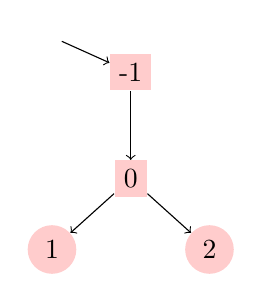
\begin{tikzpicture}[yscale=0.9]
\node (start) at (0,3) {};
\node[rectangle,fill=red!20] (-1) at (1,2.5) {-1};
\node[rectangle,fill=red!20] (0) at (1,1) {0};
\node[circle,fill=red!20] (1) at (0,0) {1};
\node[circle,fill=red!20] (2) at (2,0) {2};

\draw[->] (start)--(-1);
\draw[->] (-1)--(0);
\draw[->] (0)--(1);
\draw[->] (0)--(2);
\end{tikzpicture}
\end{center}
State~-1 is the initial state.  The states -1 and 0 are fully explored, and  states 1 and 2 are not fully explored.  The listener produces a file, the name of which is the name of the system under test with ``.tra'' as suffix (see \cite[Section 7.4]{B20}), with the following content.
\begin{verbatim}
-1 -> 0
0 -> 1
0 -> 2
1 2
\end{verbatim}
The first three lines describe the transitions.  Each line contains the source of the transition followed by the target of the transition.  The last line contains the states that are not fully explored yet.

\section{Counterexamples and Witnesses}

\bibliographystyle{plain}
\bibliography{report}

\end{document}



Bruns and Godefroid \cite{BG00} show that any partial transition system can be completed into two ``extreme'' transition systems, called the optimistic and pessimistic completions, and that model-checking a partial transition system can be reduced to model-checking its optimistic and pessimistic completions.



The idea behind the algorithm of Bruns and Godefroid \cite{BG99} is to check the partial transition system twice.  First check the system under a pessimistic interpretation, in which the value ? is understood as $\bottom$.  If the result of the check is $\top$ then return $\top$ as the 3-valued result. Then check the structure under an optimistic interpretation, in which the value ? is understood as $\top$. If the result of this check is $\bottom$ then return $\bottom$.  Otherwise return ?.

Suppose that the state space of a transition system is so large that only part of it can be explored. Bruns and Godefroid \cite{BG99} present a simple construction to define a partial transition system that represents only the explored states and transitions of this state space.  



\section{A New Semantics for CTL}

The normal semantics of CTL is described in \cite[Section~6.2.2]{BK08}.  This normal semantics is defined for a transition system $(S, Act, \rightarrow, I, AP, L)$.  Such a transition system is defined in \cite[Definition~2.1]{BK08}.  The new semantics considers a partial transition system.  A partial transition system is a tuple $(S, F, Act, \rightarrow, I, AP, L)$, where all components are defined as before and $F \subseteq S$ is a set of fully explored states.  A transition system is called partial because the states $S \setminus F$ are not fully explored yet, that is, these states \emph{have} transitions that have not been explored yet, that is, they are not part of $\rightarrow$.

Consider the following partial transition system.
\begin{center}
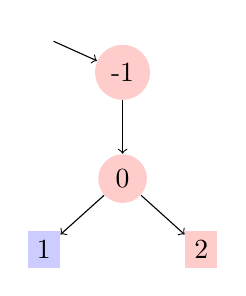
\begin{tikzpicture}[yscale=0.9]
\node (start) at (0,3) {};
\node[circle,fill=red!20] (-1) at (1,2.5) {-1};
\node[circle,fill=red!20] (0) at (1,1) {0};
\node[rectangle,fill=blue!20] (1) at (0,0) {1};
\node[rectangle,fill=red!20] (2) at (2,0) {2};

\draw[->] (start)--(-1);
\draw[->] (-1)--(0);
\draw[->] (0)--(1);
\draw[->] (0)--(2);
\end{tikzpicture}
\end{center}
State~-1 is the initial state.  The states -1 and 0 are fully explored, and  states 1 and 2 are not fully explored.  Consider, for example, the CTL formula $\exists \eventually\, \mbox{blue}$.  This formula holds in the above partial transition system, since state 1 is blue and can be reached from the initial state.  The CTL formula $\forall \always\, \mbox{red}$ does not hold for the same reason.  Now consider the CTL formula $\forall \always\, (\mbox{red} \vee \mbox{blue})$.  The above partial transition system does not provide a counterexample to this formula as all states that can be reached from the initial state are either red or blue.  However, since states 1 and 2 are not fully explored, either state may have a successor that is neither red nor blue.  So, the best we can say is ``don't know.''  Hence, whether a partial transition system satisfies a CTL formula can be answered as either yes ($\top$), no ($\bottom$), or don't know (?).

Recall that the satisfaction relation $\models$, defined in \cite[Definition~6.4]{BK08}, can be viewed as mapping a state~$s$ of a transition system and a CTL formula~$\varphi$ to a Boolean, that is, $(s, \varphi)$ is mapped to true if $s \models \varphi$ and mapped to false otherwise.  The satisfaction relation $\models$ for CTL formulas on partial transition systems can be viewed as a mapping from states and formulas to $\top$, $\bottom$, and ?.

We modify the definition of a transition system, as given in \cite[Definition~2.1]{BK08}, as follows.

\begin{definition}
A \emph{partial transition system} is a tuple $(S, F, \mathit{Act}, \rightarrow, I, \mathit{AP}, L)$ consisting of
\begin{itemize}
\item 
a \begin{franck}finite\end{franck} set $S$ of \emph{states},
\item
a set $F \subseteq S$ of \emph{fully explored states},
\item
a set $\mathit{Act}$ of \emph{actions},
\item
a transition relation $\mathord{\rightarrow} \subseteq S \times \mathit{Act} \times S$,
\item
a set $I \subseteq S$ of \emph{initial states},
\item
a set $\mathit{AP}$ of \emph{atomic propositions}, and
\item
a \emph{labelling function} $L : S \to 2^{\mathit{AP}}$.
\end{itemize}
\end{definition}

The difference between a partial transition system and an ordinary transition system is the set $F$ of fully explored states.  Since the set $\mathit{Act}$ of actions does not play in the remainder, we will drop it from the definition and simplify the transition relation to $\mathord{\rightarrow} \subseteq S \times S$. The partial transition system depicted above can be formally defined as $(S, F, \rightarrow, I, \mathit{AP}, L)$ where
\begin{itemize}
\item 
$S = \{ -1, 0, 1, 2 \}$,
\item
$F = \{ -1, 0 \}$,
\item
$\mathord{\rightarrow} = \{ (-1, 0), (0, 1), (0, 2) \}$,
\item
$I = \{ -1 \}$,
\item
$\mathit{AP} = \{ \mbox{blue}, \mbox{red} \}$, and
\item
and the function $L : S \to 2^{\mathit{AP}}$ is defined by
\begin{align*}
L(-1) & = \{ \mbox{red} \}\\
L(0) & = \{ \mbox{red} \}\\
L(1) & = \{ \mbox{blue} \}\\
L(2) & = \{ \mbox{red} \}
\end{align*}
\end{itemize} 

Due to the presence of unexplored states, we also revisit the definition of paths.  We fix an \emph{infinite} set $\mathcal{S}$ and we assume that for each partial transition system we have that $S \subseteq \mathcal{S}$.  We denote the set of nonempty and finite sequences of states in $\mathcal{S}$ by $\mathcal{S}^*$, the set of infinite sequences of states in $\mathcal{S}$ by $\mathcal{S}^{\omega}$, and the set of nonempty finite or infinite sequences of states in $\mathcal{S}$ by $\mathcal{S}^{\infty}$, that is, $\mathcal{S}^{\infty} = \mathcal{S}^* \cup \mathcal{S}^{\omega}$.

\begin{definition}
\label{definition:complete-path}
Let $(S, F, \rightarrow, I, \mathit{AP}, L)$ be a partial transition system.
\begin{itemize}
\item 
The nonempty and finite sequence $s_0 \ldots s_n$ in $\mathcal{S}^*$, where $n \geq 0$, is a complete path if $s_i \rightarrow s_{i+1}$ for all $0 \leq i < n$ and $s_n \not\rightarrow$ and $s_n \in F$.
\item 
The infinite sequence $s_0 s_1 \ldots$ in $\mathcal{S}^{\omega}$ is a complete path if $s_i \rightarrow s_{i+1}$ for all $i \geq 0$. 
\end{itemize}
\end{definition}

Note that we require that the final state of a finite complete path is fully explored.  We denote the set of complete paths that start in state $s$ by $\mathit{CoPaths}(s)$.

\begin{definition}
\label{definition:partial-path}
Let $(S, F, \rightarrow, I, \mathit{AP}, L)$ be a partial transition system.
\begin{itemize}
\item 
The nonempty and finite sequence $s_0 \ldots s_n$ in $\mathcal{S}^*$, where $n \geq 0$, is a partial path if $s_i \rightarrow s_{i+1}$ for all $0 \leq i < n$.
\end{itemize}
\end{definition}

We denote the set of partial paths that start in state $s$ by $\mathit{PaPaths}(s)$.

\begin{franck}
\begin{definition}
A partial path $s_0 \ldots s_n$ is maximal if $s_n \not\rightarrow$.
\end{definition}
\end{franck}

\begin{definition}
Let $(S, F, \rightarrow, I, \mathit{AP}, L)$ be a partial transition system.
\begin{itemize}
\item 
The nonempty and finite sequence $s_0 \ldots s_n s_{n+1} \ldots s_{n+m}$ in $\mathcal{S}^*$, where $n \geq 0$ and $m \geq 1$, is a potential path if $s_i \rightarrow s_{i+1}$ for all $0 \leq i < n$ and $s_n \not\in F$ and $s_n \not\rightarrow s_{n+1}$.
\item 
The infinite sequence $s_0 \ldots s_n s_{n+1} \ldots$ in $\mathcal{S}^{\omega}$, where $n \geq 0$, is a potential path if $s_i \rightarrow s_{i+1}$ for all $0 \leq i < n$ and $s_n \not\in F$ and $s_n \not\rightarrow s_{n+1}$.
\end{itemize}
\end{definition}

In the first case, the sequence $s_0 \ldots s_n s_{n+1} \ldots s_{n+m}$ consists of two parts: $s_0 \ldots s_n$ traverses the explored part of the partial transition system, whereas $s_{n+1} \ldots s_{n+m}$ traverses the unexplored part.  Note that we require that $s_n \not\rightarrow s_{n+1}$: otherwise $s_{n+1}$ would belong to the explored part.  Similarly, the sequence $s_0 \ldots s_n s_{n+1} \ldots$ consists of the parts $s_0 \ldots s_n$ and $s_{n+1} \ldots$.  

We denote the set of potential paths that start in state $s$ by $\mathit{PoPaths}(s)$.  We denote the set of all paths that start in state $s$ by $\mathit{Paths}(s)$, that is, $\mathit{Paths}(s) = \mathit{CoPaths}(s) \cup \mathit{PaPaths}(s) \cup \mathit{PoPaths}(s)$.  We denote the length of a path $\pi$ by $|\pi|$.  If the path $\pi$ is infinite, then $|\pi| = \omega$.

Consider the following partial transition system.
\begin{center}
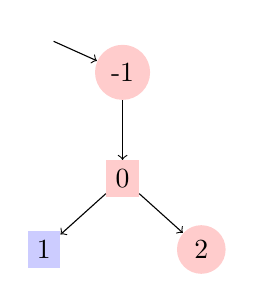
\begin{tikzpicture}[yscale=0.9]
\node (start) at (0,3) {};
\node[circle,fill=red!20] (-1) at (1,2.5) {-1};
\node[rectangle,fill=red!20] (0) at (1,1) {0};
\node[rectangle,fill=blue!20] (1) at (0,0) {1};
\node[circle,fill=red!20] (2) at (2,0) {2};

\draw[->] (start)--(-1);
\draw[->] (-1)--(0);
\draw[->] (0)--(1);
\draw[->] (0)--(2);
\end{tikzpicture}
\end{center}
We have that
\begin{align*}
\mathit{CoPaths}(-1) & = \{ -1\ 0\ 2 \}\\
\mathit{PaPaths}(-1) & = \{ -1, -1\ 0, -1\ 0\ 1, -1\ 0\ 2 \}\\
\mathit{PoPaths}(-1) & = \{\, -1\ 0\ \pi \mid \pi[0] \not\in \{ 1, 2 \} \wedge \pi \in S^{\infty} \,\} \cup \{\, -1\ 0\ 1\ \pi \mid \pi \in S^{\infty} \,\}
\end{align*}
Since state 0 is not fully explored yet, we know that this state may have more outgoing transitions than the two depicted in the above diagram.  All the potential paths starting with $-1\ 0$ do not start with either $-1\ 0\ 1$ or $-1\ 0\ 2$.  The sequence $-1\ 0\ 1$ is a partial path.  \begin{franck}The partial paths $-1\ 0\ 1$ and $-1\ 0\ 2$ are maximal.\end{franck}

\begin{franck}
\begin{definition}
For $\pi$, $\rho \in \mathit{Paths}(s)$, $\pi \sqsubseteq \rho$ if  $|\pi| \leq |\rho|$ and for all $0 \leq i < |\pi|$, $\pi[i] = \rho[i]$.
\end{definition}

\begin{proposition}
\label{proposition:partial-path-extension}
If a partial path $\pi$ is not maximal then
\begin{itemize}
\item 
there exists a maximal partial path $\rho$ such that $\pi \sqsubseteq \rho$, or
\item
there exists a complete path $\rho$ such that $\pi \sqsubseteq \rho$.
\end{itemize}
\end{proposition}
\begin{proof}
Assume that there does not exist a maximal partial path $\rho$ such that $\pi \sqsubseteq \rho$.  Let $\pi = s_0 \ldots s_n$.  Since $\pi$ is a partial path, we have that $s_i \rightarrow s_{i+1}$ for all $0 \leq i < n$.  We will prove that for all $j \geq 0$, there exists $s_{n+j} \in S$ such that $s_{n+j} \rightarrow s_{n+j+1}$ by induction on $j$.  We distinguish two cases.
\begin{itemize}
\item 
Let $j=0$.  Since $\pi$ is not maximal, $s_n \rightarrow s_{n+1}$ for some $s_{n+1} \in S$.
\item
Let $j > 0$.  By induction, $s_0 \ldots s_n s_{n+1} \ldots s_{n+j}$ is a partial path.  Obviously, $\pi \sqsubseteq s_0 \ldots s_n s_{n+1} \ldots s_{n+j}$.  By assumption, $s_0 \ldots s_n s_{n+1} \ldots s_{n+j}$ is not maximal.  Hence, there exists $s_{n+j+1} \in S$ such that $s_{n+j} \rightarrow s_{n+j+1}$.
\end{itemize}
From the above we can conclude that $s_0 \ldots s_n s_{n+1} s_{n+2} \ldots$ is a complete path with $\pi \sqsubseteq s_0 \ldots s_n s_{n+1} s_{n+2} \ldots$.
\end{proof}

\begin{proposition}
\label{proposition:partial-path-extension}
For all $\pi \in \mathit{PaPaths}(s)$ there exists $\rho \in \mathit{CoPaths}(s) \cup \mathit{PoPaths}(s)$ such that $\pi \sqsubseteq \rho$.
\end{proposition}
\begin{proof}
Towards a contradiction, assume that 
\begin{equation}
\label{equation:exists-no-extension}
\exists \pi \in \mathit{PaPaths}(s) : \forall \rho \in \mathit{CoPaths}(s) \cup \mathit{PoPaths}(s) : \pi \not\sqsubseteq \rho.
\end{equation}
We distinguish two cases.
\begin{itemize}
\item 
Assume that $\pi = s_0 \ldots s_n$ is maximal.  Then $s_n \not\rightarrow$.  Again we distinguish two cases.
\begin{itemize}
\item 
If $s_n \in F$ then $\pi \in \mathit{CoPaths}(s)$ and $\pi \sqsubseteq \pi$, contradicting (\ref{equation:exists-no-extension}).
\item
If $s_n \not\in F$ then $\pi s_n \in \mathit{PoPaths}(s)$ and $\pi \sqsubseteq \pi s_n$, contradicting (\ref{equation:exists-no-extension}).
\end{itemize}
\item
Assume that $\pi$ is not maximal. According to Proposition~\ref{proposition:partial-path-extension}, there are two cases.
\begin{itemize}
\item 
There exists a maximal partial path $\rho$ such that $\pi \sqsubseteq \rho$.  In this case we can use the same reasoning as in the first case.
\item
There exists a complete path $\rho$ such that $\pi \sqsubseteq \rho$.  This contradicts (\ref{equation:exists-no-extension}). 
\end{itemize} 
\end{itemize}
\end{proof}

\begin{proposition}
\label{proposition:there-are-paths}
For all $s \in S$, $\mathit{CoPaths}(s) \cup \mathit{PoPaths}(s) \not= \emptyset$.
\end{proposition}
\begin{proof}
First, we will show that for all $s \in S$ and $n \in \mathbb{N}$,
\begin{itemize}
\item[(a)]
$\exists \pi_n \in \mathit{CoPaths}(s) : |\pi_n| \leq n + 1$ or
\item[(a)]
$\exists \pi_n \in \mathit{PoPaths}(s) : |\pi_n| \leq n + 2$ or
\item[(b)]
$\exists \pi_n \in \mathit{PaPaths}(s) : |\pi_n| = n + 1$
\end{itemize}
and $\forall 0 \leq i < j \leq n: \pi_i \sqsubseteq \pi_j$.  We prove this by induction on $n$.  Let $s \in S$.   We distinguish the following two cases.
\begin{itemize}
\item 
Let $n = 0$.  We distinguish the following three cases.
\begin{itemize}
\item 
If $s \in F \wedge \mathit{post}(s) = \emptyset$ then $s \in \mathit{CoPaths}(s)$.
\item
If $s \not\in F$ there exists $s' \in \mathcal{S} \setminus \mathit{post}(s)$ such that $s s' \in \mathit{PoPaths}(s)$.
\item 
Otherwise, $s \in F \wedge \mathit{post}(s) \not= \emptyset$.   Then $s \in \mathit{PaPaths}(s)$.
\end{itemize} 
\item
Otherwise, $n > 0$.  We distinguish the following two cases.
\begin{itemize}
\item 
Assume $\exists \pi_{n-1} \in \mathit{CoPaths}(s) : |\pi_{n-1}| \leq n$ and  $\forall 0 \leq i < j \leq n - 1: \pi_i \sqsubseteq \pi_j$.  Then we choose $\pi_n = \pi_{n-1}$.
\item 
Assume $\exists \pi_{n-1} \in \mathit{PoPaths}(s) : |\pi_{n-1}| \leq n + 1$ and  $\forall 0 \leq i < j \leq n - 1: \pi_i \sqsubseteq \pi_j$.  Then we choose $\pi_n = \pi_{n-1}$.
\item
Otherwise, $\exists \pi_{n-1} \in \mathit{PaPaths}(s) : |\pi_{n-1}| = n$  and $\forall 0 \leq i < j \leq n - 1: \pi_i \sqsubseteq \pi_j$.  Let $s' = \pi_{n-1}[n-1]$.  We distinguish the following three cases.
\begin{itemize}
\item 
If $s' \in F \wedge \mathit{post}(s') = \emptyset$ then $\pi_{n-1} \in \mathit{CoPaths}(s)$.  Then we choose $\pi_n = \pi_{n-1}$.
\item
If $s' \not\in F$ there exists $s'' \in \mathcal{S} \setminus \mathit{post}(s')$ such that $\pi_{n-1} s'' \in \mathit{PoPaths}(s)$.  Then we choose $\pi_n = \pi_{n-1} s''$.
\item
Otherwise, $s' \in F \wedge \mathit{post}(s') \not= \emptyset$.  Let $s'' \in \mathit{post}(s')$.  In this case, $\pi_{n-1} s'' \in \mathit{PaPaths}(s)$ and, therefore, we choose $\pi_n = \pi_{n-1} s''$.
\end{itemize}
\end{itemize}
\end{itemize}
From the above we can conclude the following.  Let $s \in S$.  Then either
\[
\exists n \in \mathbb{N} : \exists \pi_n \in \mathit{CoPaths}(s) \cup \mathit{PoPaths}(s) 
\]
or
\begin{align*}
\forall n \in \mathbb{N} : \exists \pi_n \in \mathit{PaPaths}(s) :\, & |\pi_n| = n + 1 \wedge \forall 0 \leq i < j \leq n: \pi_i \sqsubseteq \pi_j.
\end{align*}
In the latter case, for $\pi_{\omega} \in S^{\omega}$ with $\pi_{\omega}[i] = \pi_i[i]$ we have that $\pi_{\omega} \in \mathit{CoPaths}(s)$.
\end{proof}
\end{franck}

A partial transition system in which all states are fully explored, that is, an ordinary transition system, has no potential paths.  Furthermore, each partial path can be extended to a complete path.

\begin{proposition}
\label{proposition:no-potential-paths}
If $F= S$ then for all $s \in S$, $\mathit{PoPaths}(s) = \emptyset$.
\end{proposition}
\begin{proof}\ 
Immediate from the definition of potential paths ($s_n \not\in F$).
\end{proof}

The satisfaction relation $\models$ for CTL for ordinary transition systems is defined in \cite[Definition~6.4]{BK08}.  It can be viewed as a function $\satisfaction{\ }$ that maps each CTL formula and state of a transition system to either true of false, that is, for each state formula $\varphi$ and state $s$,
\[
s \models \varphi \mbox{ iff } \satisfaction{\varphi}(s) = \mbox{true}.
\]

To deal with partial transition systems, we extend the range of the function $\satisfaction{\ }$.  Given a formula $\varphi$ and a state $s$, we have that either
\begin{itemize}
\item 
$\satisfaction{\varphi}(s) = \top$: the formula $\varphi$ holds in the state $s$,
\item
$\satisfaction{\varphi}(s) = \bottom$: the formula $\varphi$ does not hold in the state $s$, or
\item
$\satisfaction{\varphi}(s) = \mathord{?}$: we cannot determine whether the formula $\varphi$ holds in the state $s$ since some states, relevant to $\varphi$,  have not been explored.
\end{itemize}

For example, consider the partial transition system depicted above.  Consider the formula $\forall \nxt \mbox{red}$.  We have that $\satisfaction{\forall \nxt \mbox{red}}(-1) = \top$ since the state $-1$ is fully explored and all its successor states are red.  Furthermore, $\satisfaction{\forall \nxt \mbox{red}}(0) = \bottom$ since one of the  successor states of state 0 is not red.  Finally, $\satisfaction{\forall \nxt \mbox{red}}(1) = \mathord{?}$ since the state 1 is not fully explored and it does not have a successor that is not red.

We denote the set of three values, $\top$, $\bottom$ and $?$ by $\mathbb{V}$, that is,
\[
\mathbb{V} = \{ \top, \bottom, \mathord{?} \}.
\]
We can extend the usual Boolean operators to $\mathbb{V}$ as follows.  Negation is captured in the following table.
\[
\begin{array}{c|c}
v & \neg v\\\hline
\top & \bottom\\
\bottom & \top\\
\mathord{?} & \mathord{?}
\end{array}
\]
Conjunction is defined as follows.
\[
\begin{array}{cc|ccc}
\multicolumn{2}{c|}{v \wedge w} & & w &\\
&& \top & \bottom & \mathord{?}\\\hline
& \top & \top & \bottom & \mathord{?}\\
v & \bottom & \bottom & \bottom & \bottom\\
& \mathord{?} & \mathord{?} & \bottom & \mathord{?}
\end{array}
\]
Disjunction is defined as follows.
\[
\begin{array}{cc|ccc}
\multicolumn{2}{c|}{v \vee w} & & w &\\
&& \top & \bottom & \mathord{?}\\\hline
& \top & \top & \top & \top\\
v & \bottom & \top & \bottom & \mathord{?}\\
& \mathord{?} & \top & \mathord{?} & \mathord{?}
\end{array}
\]
Implication is defined as follows.
\[
\begin{array}{cc|ccc}
\multicolumn{2}{c|}{v \rightarrow w} & & w &\\
&& \top & \bottom & \mathord{?}\\\hline
& \top & \top & \bottom & ?\\
v & \bottom & \top & \top & \top\\
& \mathord{?} & \top & ? & ?
\end{array}
\]
Equivalence is defined as follows.
\[
\begin{array}{cc|ccc}
\multicolumn{2}{c|}{v \leftrightarrow w} & & w &\\
&& \top & \bottom & \mathord{?}\\\hline
& \top & \top & \bottom & ?\\
v & \bottom & \bottom & \top & ?\\
& \mathord{?} & ? & ? & ?
\end{array}
\]

We denote the set of CTL formulas by $\mathit{CTL}$.

\begin{definition}
Let $(S, F, \rightarrow, I, \mathit{AP}, L)$ be a partial transition system.  The function 
\[
\satisfaction{\ } : \mathit{CTL} \to S \to \mathbb{V}
\] 
is defined by structural induction on the CTL formula as follows.
\begin{itemize}
\item 
$\satisfaction{a}(s) = \left \{
\begin{array}{ll}
\top & \mbox{if $a \in L(s)$}\\
\bottom & \mbox{otherwise}
\end{array}\right .
$
\item 
$\satisfaction{\TRUE}(s) = \top$ 
\item 
$\satisfaction{\FALSE}(s) = \bottom$ 
\item 
$\satisfaction{\neg \varphi}(s) = \neg \satisfaction{\varphi}(s)$ 
\item 
$\satisfaction{\varphi \wedge \psi}(s) = \satisfaction{\varphi}(s) \wedge \satisfaction{\psi}(s)$ 
\item 
$\satisfaction{\varphi \vee \psi}(s) = \satisfaction{\varphi}(s) \vee \satisfaction{\psi}(s)$ 
\item 
$\satisfaction{\varphi \rightarrow \psi}(s) = \satisfaction{\varphi}(s) \rightarrow \satisfaction{\psi}(s)$ 
\item 
$\satisfaction{\varphi \leftrightarrow \psi}(s) = \satisfaction{\varphi}(s) \leftrightarrow \satisfaction{\psi}(s)$ 
\begin{franck}
\item
$\satisfaction{\forall \nxt \varphi}(s) = \left \{
\begin{array}{ll}
\top & \mbox{if $\forall \pi \in \mathit{Paths}(s) : |\pi| > 1 \Rightarrow \satisfaction{\varphi}(\pi[1]) = \top$}\\
\bottom & \mbox{if $\exists \pi \in \mathit{CoPaths}(s) \cup \mathit{PaPaths}(s) : |\pi| > 1 \wedge \satisfaction{\varphi}(\pi[1]) = \bottom$}\\
& \mbox{or $\mathit{PoPaths}(s) \not= \emptyset \wedge \forall \pi \in \mathit{PoPaths}(s) : |\pi| > 1 \wedge \satisfaction{\varphi}(\pi[1]) = \bottom$}\\
? & \mbox{otherwise}
\end{array}
\right .
$
\item
$\satisfaction{\exists \nxt \varphi}(s) = \left \{
\begin{array}{ll}
\top & \mbox{if $\exists \pi \in \mathit{CoPaths}(s) \cup \mathit{PaPaths}(s) : |\pi| > 1 \wedge \satisfaction{\varphi}(\pi[1]) = \top$}\\
& \mbox{or $\mathit{PoPaths}(s) \not= \emptyset \wedge \forall \pi \in \mathit{PoPaths}(s) : |\pi| > 1 \wedge \satisfaction{\varphi}(\pi[1]) = \top$}\\
\bottom & \mbox{if $\forall \pi \in \mathit{Paths}(s) : |\pi| > 1 \Rightarrow \satisfaction{\varphi}(\pi[1]) = \bottom$}\\
? & \mbox{otherwise}
\end{array}
\right .
$
\item
$\satisfaction{\forall \always \varphi}(s) = \left \{
\begin{array}{ll}
\top & \mbox{if $\forall \pi \in \mathit{Paths}(s) :  \forall 0 \leq i < |\pi| : \satisfaction{\varphi}(\pi[i]) = \top$}\\
\bottom & \mbox{if $\exists \pi \in \mathit{CoPaths}(s) \cup \mathit{PaPaths}(s) : \exists 0 \leq i < |\pi| : \satisfaction{\varphi}(\pi[i]) = \bottom$}\\
%& \mbox{or $\mathit{PoPaths}(s) \not= \emptyset \wedge \forall \pi \in \mathit{PoPaths}(s) : \exists 0 \leq i < |\pi| : \satisfaction{\varphi}(\pi[i]) = \bottom$}\\
? & \mbox{otherwise}
\end{array}
\right .
$
\item
$\satisfaction{\exists \always \varphi}(s) = \left \{
\begin{array}{ll}
\top & \mbox{if $\exists \pi \in \mathit{CoPaths}(s) : \forall 0 \leq i < |\pi| : \satisfaction{\varphi}(\pi[i]) = \top$}\\
& \mbox{or $\mathit{PoPaths}(s) \not= \emptyset \wedge \forall \pi \in \mathit{PoPaths}(s) : \forall 0 \leq i < |\pi| : \satisfaction{\varphi}(\pi[i]) = \top$}\\
\bottom & \mbox{if $\forall \pi \in \mathit{CoPaths}(s) \cup \mathit{PoPaths}(s) : \exists 0 \leq i < |\pi| : \satisfaction{\varphi}(\pi[i]) = \bottom$}\\
? & \mbox{otherwise}
\end{array}
\right .
$
\item
$\satisfaction{\forall \eventually \varphi}(s) = \left \{
\begin{array}{ll}
\top & \mbox{if $\forall \pi \in \mathit{CoPaths}(s) \cup \mathit{PoPaths}(s) : \exists 0 \leq i < |\pi| : \satisfaction{\varphi}(\pi[i]) = \top$}\\
\bottom & \mbox{if $ \exists \pi \in \mathit{CoPaths}(s) :  \forall 0 \leq i < |\pi| : \satisfaction{\varphi}(\pi[i]) = \bottom$}\\
& \mbox{or $\mathit{PoPaths}(s) \not= \emptyset \wedge \forall \pi \in \mathit{PoPaths}(s) : \forall 0 \leq i < |\pi| : \satisfaction{\varphi}(\pi[i]) = \bottom$}\\
? & \mbox{otherwise}
\end{array}
\right .
$
\item
$\satisfaction{\exists \eventually \varphi}(s) = \left \{
\begin{array}{ll}
\top & \mbox{if $\exists \pi \in \mathit{CoPaths}(s) \cup \mathit{PaPaths}(s) : \exists0 \leq i < |\pi| : \satisfaction{\varphi}(\pi[i]) = \top$}\\
%& \mbox{or $\mathit{PoPaths}(s) \not= \emptyset \wedge \forall \pi \in \mathit{PoPaths}(s) : \exists 0 \leq i < |\pi| : \satisfaction{\varphi}(\pi[i]) = \top$}\\
\bottom & \mbox{if $\forall \pi \in \mathit{Paths}(s) : \forall 0 \leq i < |\pi| : \satisfaction{\varphi}(\pi[i]) = \bottom$}\\
? & \mbox{otherwise}
\end{array}
\right .
$
\item
$\satisfaction{\forall \varphi \until \psi}(s) = $ \textcolor{blue}{details still need to be added here.}
\item
%\begin{align*}
$\satisfaction{\exists \varphi \until \psi}(s)$ = \textcolor{blue}{details still need to be added here.}
%\\
%& \left \{
%\begin{array}{ll}
%\top & \mbox{if $\exists \pi \in \mathit{CoPaths}(s) \cup \mathit{PaPaths}(s) : \exists 0 \leq i < |\pi| : \satisfaction{\psi}(\pi[i]) = \top \wedge \forall 0 \leq i < j : \satisfaction{\varphi}(\pi[j]) = \top$}\\
%& \mbox{of $\mathit{PoPaths}(s) \not= \emptyset \wedge \forall \pi \in \mathit{PoPaths}(s) : \exists 0 \leq i < |\pi| : \satisfaction{\psi}(\pi[i]) = \top \wedge \forall 0 \leq i < j : \satisfaction{\varphi}(\pi[j]) = \top$}\\
%\bottom & \mbox{if \textcolor{blue}{incomplete}}\\
%? & \mbox{otherwise}
%\end{array}
%\right .
%\end{align*}
\end{franck}
\end{itemize}
\end{definition}

Which paths to consider for the formulas that start with a quantifier is subtle.  Next, we discuss our choices and motivate them by means of examples.

\subsection*{$\satisfaction{\forall \nxt \varphi}(s) = \top$}

To conclude that $\satisfaction{\forall \nxt \varphi}(s)$ is true, we need that all successors of state~$s$ satisfy $\varphi$.  If state~$s$ is fully explored, we need to consider all successors:
\[
\{\, \pi[1] \mid \pi \in \mathit{CoPaths}(s) \cup \mathit{PaPaths}(s) \,\}
= \{\, \pi[1] \mid \pi \in \mathit{Paths}(s) \,\}.
\]

Consider the following partial transition system.
\begin{center}
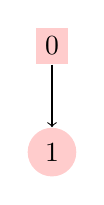
\begin{tikzpicture}[yscale=0.9]
\node[rectangle,fill=red!20] (0) at (1,2.5) {0};
\node[circle,fill=red!20] (1) at (1,1) {1};

\draw[->] (0)--(1);
\end{tikzpicture}
\end{center}
Since state~0 is not fully explored, state~0 has transitions to states other than state~1.  Those other states may not be red and, hence, we do not know whether  $\forall \nxt \mbox{red}$ holds in state~0.  Therefore, for a non-fully explored state~$s$, we consider also all potential successors of state~$s$ when determining if $\forall \nxt \varphi$ holds in $s$:
\[
\{\, \pi[1] \mid \pi \in \mathit{Paths}(s) \,\}
\]

\subsection*{$\satisfaction{\forall \nxt \varphi}(s) = \bottom$}

We can conclude that $\satisfaction{\forall \nxt \varphi}(s)$ is false, if we find a counterexample, that is, a successor of state~$s$ in which $\varphi$ does not hold.  Consider the following partial transition system.
\begin{center}
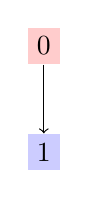
\begin{tikzpicture}[yscale=0.9]
\node[rectangle,fill=red!20] (0) at (1,2.5) {0};
\node[rectangle,fill=blue!20] (1) at (1,1) {1};

\draw[->] (0)--(1);
\end{tikzpicture}
\end{center}
Since state~0 transitions to a state that is not red, we can conclude that $\forall \nxt \mbox{red}$ does not hold in state~0.  Because state~1 is not fully explored, it has unexplored outgoing transitions.  Hence, the path $0\ 1$ is not complete.  Therefore, we consider both complete and partial paths starting from state~$s$ when determining if $\satisfaction{\forall \nxt \varphi}(s) = \bottom$.

Consider the following partial transition system.
\begin{center}
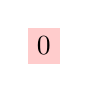
\begin{tikzpicture}[yscale=0.9]
\node[rectangle,fill=red!20] (0) at (1,2.5) {0};
\end{tikzpicture}
\end{center}
Since state~0 is not fully explored, it has transitions.  As a consequence, the formula $\forall \nxt \FALSE$ does not holds in state~0.  More generally, if there are potential paths starting of state~$s$ and each second state of all those potential paths does not satisfy $\varphi$, then we can conclude that $\forall \nxt \varphi$ does not holds in $s$.

\subsection*{$\satisfaction{\exists \nxt \varphi}(s) = \top$}

We can conclude that $\satisfaction{\exists \nxt \varphi}(s)$ is true, if we find a witness, that is, a successor of state~$s$ that satisfies $\varphi$.  Consider the following partial transition system.
\begin{center}
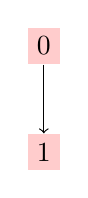
\begin{tikzpicture}[yscale=0.9]
\node[rectangle,fill=red!20] (0) at (1,2.5) {0};
\node[rectangle,fill=red!20] (1) at (1,1) {1};

\draw[->] (0)--(1);
\end{tikzpicture}
\end{center}
Since state~0 transitions to a state that is red, we can conclude that $\exists \nxt \mbox{red}$ holds in state~0.  Because state~1 is not fully explored, it has unexplored outgoing transitions.  Hence, the path $0\ 1$ is not complete.  Therefore, we consider both complete and partial paths starting from state~$s$ when determining if $\satisfaction{\exists \nxt \varphi}(s) = \top$.  Obviously, potential paths should not be considered.

Consider the following partial transition system.
\begin{center}
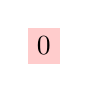
\begin{tikzpicture}[yscale=0.9]
\node[rectangle,fill=red!20] (0) at (1,2.5) {0};
\end{tikzpicture}
\end{center}
Since state~0 is not fully explored, it has transitions.  As a consequence, the formula $\forall \nxt \TRUE$ holds in state~0.  More generally, if there are potential paths starting of state~$s$ and each second state of all those potential paths satifies $\varphi$, then we can conclude that $\forall \nxt \varphi$ holds in $s$.

\subsection*{$\satisfaction{\exists \nxt \varphi}(s) = \bottom$}

To conclude that $\satisfaction{\exists \nxt \varphi}(s)$ is false, we need that none of the successors of state~$s$ satisfy $\varphi$.  If state~$s$ is fully explored, we need to consider all successors:
\[
\{\, \pi[1] \mid \pi \in \mathit{CoPaths}(s) \cup \mathit{PaPaths}(s) \,\}
= \{\, \pi[1] \mid \pi \in \mathit{Paths}(s) \,\}.
\]

Consider the following partial transition system.
\begin{center}
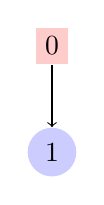
\begin{tikzpicture}[yscale=0.9]
\node[rectangle,fill=red!20] (0) at (1,2.5) {0};
\node[circle,fill=blue!20] (1) at (1,1) {1};

\draw[->] (0)--(1);
\end{tikzpicture}
\end{center}
Since state~0 is not fully explored, state~0 may have transitions to states other than state~1.  Those other states may be red and, hence, we do not know whether  $\exists \nxt \mbox{red}$ does not hold in state~0.  Therefore, for a non-fully explored state~$s$, we consider all actual and potential successors of state~$s$ when determining if $\exists \nxt \varphi$ does not hold in $s$:
\[
\{\, \pi[1] \mid \pi \in \mathit{Paths}(s) \,\}
\]

\subsection*{$\satisfaction{\forall \always \varphi}(s) = \top$}

To conclude that $\satisfaction{\forall \always \varphi}(s)$ is true, we need that all states reachable from state~$s$ satisfy $\varphi$.

Consider the following partial transition system.
\begin{center}
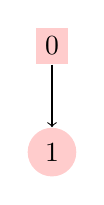
\begin{tikzpicture}[yscale=0.9]
\node[rectangle,fill=red!20] (0) at (1,2.5) {0};
\node[circle,fill=red!20] (1) at (1,1) {1};

\draw[->] (0)--(1);
\end{tikzpicture}
\end{center}
States different from state~1 that are reachable from state~0 by transitions that have not been explored yet may not be red in which case $\forall \always \mbox{red}$ does not hold.  Therefore, we consider all paths, including the potential paths, starting from state~$s$ when determining if $\satisfaction{\forall \always \varphi}(s) = \top$.

\subsection*{$\satisfaction{\forall \always \varphi}(s) = \bottom$}

If we can find a counterexample, that is, a path starting in state~$s$ that contains a state that does not satisfy $\varphi$, then we can conclude that $\satisfaction{\forall \always \varphi}(s)$ is false.  We consider both complete and partial paths, but not potential paths.

%Consider the following partial transition system.
%\begin{center}
%\begin{tikzpicture}[yscale=0.9]
%\node[rectangle,fill=red!20] (0) at (1,2.5) {0};
%\end{tikzpicture}
%\end{center}
%Since state~0 is not fully explored, it has transitions.  If all potential paths starting of state~0 contain a state that does not satisfy $\varphi$, then we can conclude that $\forall \always \varphi$ does not hold in state~0.

\subsection*{$\satisfaction{\exists \always \varphi}(s) = \top$}

If we can find a witness, that is, a complete path starting in state~$s$ of which all states satisfy $\varphi$, then we can conclude that $\satisfaction{\exists \always \varphi}(s)$ is true.

Consider the following partial transition system.
\begin{center}
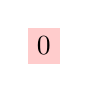
\begin{tikzpicture}[yscale=0.9]
\node[rectangle,fill=red!20] (0) at (1,2.5) {0};
\end{tikzpicture}
\end{center}
Since state~0 is not fully explored, it has transitions.  As a consequence, the formula $\exists \always \TRUE$ holds in state~0.  More generally, if there are potential paths starting of state~$s$ and all the states of those potential paths satify $\varphi$, then we can conclude that $\exists \always \varphi$ holds in $s$.

\subsection*{$\satisfaction{\exists \always \varphi}(s) = \bottom$}

To conclude that $\satisfaction{\exists \always \varphi}(s)$ is false, we need that each path that starts in state~$s$ contains a state that does not satisfy $\varphi$.  Consider the following partial transition system.
\begin{center}
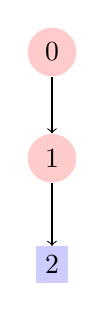
\begin{tikzpicture}[yscale=0.9]
\node[circle,fill=red!20] (0) at (1,2.5) {0};
\node[circle,fill=red!20] (1) at (1,1) {1};
\node[rectangle,fill=blue!20] (2) at (1,-0.5) {2};

\draw[->] (0)--(1);
\draw[->] (1)--(2);
\end{tikzpicture}
\end{center}
Since each path starting from state~0 contains state~2, which is blue, we can conclude that $\exists \always \mbox{red}$ does not hold in state~0.  Note that we should consider both complete paths as well as potential paths.  Partial paths should not be considered.  For example, the partial path $0\ 1$ contains only red states.

\subsection*{$\satisfaction{\forall \eventually \varphi}(s) = \top$}

To conclude that $\satisfaction{\forall \eventually \varphi}(s)$ is true, we need that each path contains a state that satisfies $\varphi$.  Consider the following partial transition system.
\begin{center}
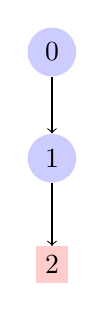
\begin{tikzpicture}[yscale=0.9]
\node[circle,fill=blue!20] (0) at (1,2.5) {0};
\node[circle,fill=blue!20] (1) at (1,1) {1};
\node[rectangle,fill=red!20] (2) at (1,-0.5) {2};

\draw[->] (0)--(1);
\draw[->] (1)--(2);
\end{tikzpicture}
\end{center}
Since each path starting from state~0 contains state~2, which is red, we can conclude that $\forall \eventually \mbox{red}$ holds in state~0.  Note that we should consider both complete paths as well as potential paths.  Partial paths should not be considered.  For example, the partial path $0\ 1$ does not contain any red states.

\subsection*{$\satisfaction{\forall \eventually \varphi}(s) = \bottom$}

If we can find a counterexample, that is, a path starting in state~$s$ of which all states do not satisfy $\varphi$, then we can conclude that $\satisfaction{\forall \eventually \varphi}(s)$ is false.  Consider the following partial transition system.
\begin{center}
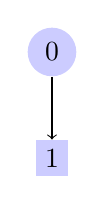
\begin{tikzpicture}[yscale=0.9]
\node[circle,fill=blue!20] (0) at (1,2.5) {0};
\node[rectangle,fill=blue!20] (1) at (1,1) {1};

\draw[->] (0)--(1);
\end{tikzpicture}
\end{center}
The partial path $0\ 1$ may be the prefix of a complete path that includes red states and, hence, we cannot conclude that $\satisfaction{\forall \eventually \mbox{red}}(0) = \bottom$.  Therefore, we consider complete paths only when determining if $\satisfaction{\forall \eventually \varphi}(s) = \bottom$.

Consider the following partial transition system.
\begin{center}
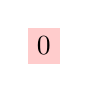
\begin{tikzpicture}[yscale=0.9]
\node[rectangle,fill=red!20] (0) at (1,2.5) {0};
\end{tikzpicture}
\end{center}
Since state~0 is not fully explored, it has transitions.  As a consequence, the formula $\forall \eventually \FALSE$ does not hold in state~0.  More generally, if there are potential paths starting of state~$s$ and all the states of those potential paths do not satify $\varphi$, then we can conclude that $\forall \eventually \varphi$ does not hold in $s$.

\subsection*{$\satisfaction{\exists \eventually \varphi}(s) = \top$}

To conclude that $\satisfaction{\exists \eventually \varphi}(s)$ is true, we need to find a witness, that is, a path starting in state~$s$ that contains a state that satisfies $\varphi$.  The path can either be complete or partial.

\subsection*{$\satisfaction{\exists \eventually \varphi}(s) = \bottom$}

To conclude that $\satisfaction{\exists \eventually \varphi}(s)$ is false, no path starting in state~$s$ should contain a state that satisfies $\varphi$.  Hence, we need to consider complete, partial, and potential paths.

\begin{franck}
\subsection*{$\satisfaction{\exists \varphi \until \psi}(s) = \top$}

To conclude that $\satisfaction{\exists \varphi \until \psi}(s)$ is true, we either need a witness, that is, a path starting in state~$s$ that contains a state that satisfies $\psi$ and all preceding states satisfy $\varphi$.  The path can either be complete or partial.  Or there exists at least one potential path and all potential paths contain a state that satisfies $\psi$ and all preceding states satisfy $\varphi$.

\begin{align*}
& \exists \pi \in \mathit{CoPaths}(s) \cup \mathit{PaPaths}(s) : \exists 0 \leq i < |\pi| : \satisfaction{\psi}(\pi[i]) = \top \wedge \forall 0 \leq i < j : \satisfaction{\varphi}(\pi[j]) = \top \vee\\
& \mathit{PoPaths}(s) \not= \emptyset \wedge \forall \pi \in \mathit{PoPaths}(s) : \exists 0 \leq i < |\pi| : \satisfaction{\psi}(\pi[i]) = \top \wedge \forall 0 \leq i < j : \satisfaction{\varphi}(\pi[j]) = \top
\end{align*}

\end{franck}

\section{Existential Normal Form}

In \cite[Definition~6.13]{BK08}, an existential normal form has been introduced.  It restricts the syntax of CTL.  In particular, it restricts to existential quantifiers, eliminating the universal quantifiers.  Furthermore, in \cite[Theorem~6.14]{BK08}, it is shown that for each CTL formula there exists an equivalent CTL formula in existential normal.  Below, we extend these results to the setting of partial transition systems.

\begin{definition}
Let $\mathit{AP}$ be the set of atomic propositions.  The set of CTL formulas in existential normal form is defined by the following grammar.
\[
\varphi
::= a
\mid \neg \varphi
\mid \varphi \wedge \varphi
\mid \exists \nxt \varphi
\mid \exists \always \varphi
\mid \exists \eventually \varphi
\mid \exists \varphi \until \varphi
%\mid \forall \varphi \until \varphi
\]
where $a \in \mathit{AP}$.
\end{definition}

Next, we define equivalence of CTL formulas.

\begin{definition}
For CTL formulas $\varphi$ and $\psi$, 
\[
\varphi \equiv \psi \mbox{ if } \satisfaction{\varphi}(s) = \satisfaction{\psi}(s) \mbox{ for all partial transition systems and } s \in S.
\]
\end{definition}

\begin{proposition}
Let $a \in \mathit{AP}$.  For CTL formulas $\varphi$ and $\psi$, 
\begin{enumerate}
\item 
$\TRUE \equiv a \vee \neg a$
\item 
$\FALSE \equiv a \wedge \neg a$
\item
$\varphi \vee \psi \equiv \neg(\neg \varphi \wedge \neg \psi)$
\item
$\varphi \rightarrow \psi \equiv \neg \varphi \vee \psi$
\item
$\varphi \leftrightarrow \psi \equiv (\varphi \rightarrow \psi) \wedge (\psi \rightarrow \varphi)$
\item
$\forall \nxt \varphi \equiv \neg \exists \nxt \neg \varphi$
\item
$\forall \always \varphi \equiv \neg \exists \eventually \neg \varphi$
\item
$\forall \eventually \varphi \equiv \neg \exists \always \neg \varphi$
\item
\begin{franck}
$\forall \varphi \until \psi \equiv (\neg \exists (\neg \psi) \until (\neg \varphi \wedge \neg \psi)) \wedge \neg \exists \always \neg \psi$
\end{franck}
\end{enumerate}
\end{proposition}
\begin{proof}
Let $(S, F, \rightarrow, I, \mathit{AP}, L)$ be a partial transition system and let $s \in S$.
\begin{enumerate}
\item 
If $a \in L(s)$, then
\[
\satisfaction{\TRUE}(s) = \top = \top \vee \neg \top = \satisfaction{a}(s) \vee \neg \satisfaction{a}(s) = \satisfaction{a \vee \neg a}(s).
\]
Otherwise,
\[
\satisfaction{\TRUE}(s) = \top = \bottom \vee \neg \bottom = \satisfaction{a}(s) \vee \neg \satisfaction{a}(s) = \satisfaction{a \vee \neg a}(s).
\]
\item
If $a \in L(s)$, then
\[
\satisfaction{\FALSE}(s) = \bottom = \top \wedge \neg \top = \satisfaction{a}(s) \wedge \neg \satisfaction{a}(s) = \satisfaction{a \wedge \neg a}(s).
\]
Otherwise,
\[
\satisfaction{\FALSE}(s) = \bottom = \bottom \wedge \neg \bottom = \satisfaction{a}(s) \wedge \neg \satisfaction{a}(s) = \satisfaction{a \wedge \neg a}(s).
\]
\item
It suffices to show that $v \vee w = \neg(\neg v \wedge \neg w)$ for all $v$, $w \in \mathbb{V}$.

\[
\begin{array}{ll|lll|l}
v     & w     & \neg v & \neg w & \neg v \wedge \neg w & \neg(\neg v \wedge \neg w)\\\hline
\top  & \top  & \bottom  & \bottom  & \bottom                & \top\\
\bottom & \top  & \top   & \bottom  & \bottom                & \top\\
?     & \top  & ?      & \bottom  & \bottom                & \top\\
\top  & \bottom & \bottom  & \top   & \bottom                & \top\\
\bottom & \bottom & \top   & \top   & \top                 & \bottom\\
?     & \bottom & ?      & \top   & ?                    & ?\\
\top  & ?     & \bottom  & ?      & \bottom                & \top\\
\bottom & ?     & \top   & ?      & ?                    & ?\\
?     & ?     & ?      & ?      & ?                    & ?
\end{array}
\]
\item
It suffices to show that $v \rightarrow w = \neg v \vee w$ for all $v$, $w \in \mathbb{V}$.

\[
\begin{array}{ll|l|l}
v     & w     & \neg v & \neg v \vee w\\\hline
\top  & \top  & \bottom  & \top\\
\bottom & \top  & \top   & \top\\
?     & \top  & ?      & \top\\
\top  & \bottom & \bottom  & \bottom\\
\bottom & \bottom & \top   & \top\\
?     & \bottom & ?      & ?\\
\top  & ?     & \bottom  & ?\\
\bottom & ?     & \top   & \top\\
?     & ?     & ?      & ?
\end{array}
\]
\item
It suffices to show that $v \leftrightarrow w = (v \rightarrow w) \wedge (w \rightarrow v)$ for all $v$, $w \in \mathbb{V}$.

\[
\begin{array}{ll|ll|l}
v     & w     & v \rightarrow w & w \rightarrow v & (v \rightarrow w) \wedge (w \rightarrow v)\\\hline
\top  & \top  & \top  & \top  & \top\\
\bottom & \top  & \top  & \bottom & \bottom\\
?     & \top  & \top  & ?     & ?\\
\top  & \bottom & \bottom & \top  & \bottom\\
\bottom & \bottom & \top  & \top  & \top\\
?     & \bottom & ?     & \top  & ?\\
\top  & ?     & ?     & \top  & ?\\
\bottom & ?     & \top  & ?     & ?\\
?     & ?     & ?     & ?     & ?
\end{array}
\]
\item
Since
\begin{align*}
\satisfaction{\forall \nxt \varphi}(s) = \top
\mbox{ iff } & \forall \pi \in \mathit{Paths}(s) : |\pi| > 1 \Rightarrow \satisfaction{\varphi}(\pi[1]) = \top\\
\mbox{ iff } & \forall \pi \in \mathit{Paths}(s) : |\pi| > 1 \Rightarrow \satisfaction{\neg \varphi}(\pi[1]) = \bottom\\
\mbox{ iff } & \satisfaction{\exists \nxt \neg \varphi}(s) = \bottom\\
\mbox{ iff } & \satisfaction{\neg \exists \nxt \neg \varphi}(s) = \top
\end{align*}
and
\begin{align*}
\satisfaction{\forall \nxt \varphi}(s) = \bottom
\mbox{ iff } & (\exists \pi \in \mathit{CoPaths}(s) \cup \mathit{PaPaths}(s) : |\pi| > 1 \wedge \satisfaction{\varphi}(\pi[1]) = \bottom) \vee\\
& (\mathit{PoPaths}(s) \not= \emptyset \wedge \forall \pi \in \mathit{PoPaths}(s) : |\pi| > 1 \wedge \satisfaction{\varphi}(\pi[1]) = \bottom)\\
\mbox{ iff } & (\exists \pi \in \mathit{CoPaths}(s) \cup \mathit{PaPaths}(s) : |\pi| > 1 \wedge \satisfaction{\neg \varphi}(\pi[1]) = \top) \vee\\
& (\mathit{PoPaths}(s) \not= \emptyset \wedge \forall \pi \in (\mathit{PoPaths}(s) : |\pi| > 1 \wedge \satisfaction{\neg \varphi}(\pi[1]) = \top)\\
\mbox{ iff } & \satisfaction{\exists \nxt \neg \varphi}(s) = \top\\
\mbox{ iff } & \satisfaction{\neg \exists \nxt \neg \varphi}(s) = \bottom
\end{align*}
we can conclude that $\forall \nxt \varphi \equiv \neg \exists \nxt \neg \varphi$.
\item
Since
\begin{align*}
\satisfaction{\forall \always \varphi}(s) = \top
\mbox{ iff } & \forall \pi \in \mathit{Paths}(s) : \forall 0 \leq i < |\pi| : \satisfaction{\varphi}(\pi[i]) = \top\\
\mbox{ iff } & \forall \pi \in \mathit{Paths}(s) : \forall 0 \leq i < |\pi| : \satisfaction{\neg \varphi}(\pi[i]) = \bottom\\
\mbox{ iff } & \satisfaction{\exists \eventually \neg \varphi}(s) = \bottom\\
\mbox{ iff } & \satisfaction{\neg \exists \eventually \neg \varphi}(s) = \top
\end{align*}
and
\begin{align*}
\satisfaction{\forall \always \varphi}(s) = \bottom
\mbox{ iff } & \exists \pi \in \mathit{CoPaths}(s) \cup \mathit{PaPaths}(s) : \exists 0 \leq i < |\pi| : \satisfaction{\varphi}(\pi[i]) = \bottom\\
\mbox{ iff } & \exists \pi \in \mathit{CoPaths}(s) \cup \mathit{PaPaths}(s) : \exists 0 \leq i < |\pi| : \satisfaction{\neg \varphi}(\pi[i]) = \top\\
\mbox{ iff } & \satisfaction{\exists \eventually \neg \varphi}(s) = \top\\
\mbox{ iff } & \satisfaction{\neg \exists \eventually \neg \varphi}(s) = \bottom
\end{align*}
we can conclude that $\forall \always \varphi \equiv \neg \exists \eventually \neg \varphi$.
\item
Since
\begin{align*}
\satisfaction{\forall \eventually \varphi}(s) = \top
\mbox{ iff } & \forall \pi \in \mathit{CoPaths}(s) \cup \mathit{PoPaths}(s) : \exists 0 \leq i < |\pi| : \satisfaction{\varphi}(\pi[i]) = \top\\
\mbox{ iff } & \forall \pi \in \mathit{CoPaths}(s) \cup \mathit{PoPaths}(s) : \exists 0 \leq i < |\pi| : \satisfaction{\neg \varphi}(\pi[i]) = \bottom\\
\mbox{ iff } & \satisfaction{\exists \always \neg \varphi}(s) = \bottom\\
\mbox{ iff } & \satisfaction{\neg \exists \always \neg \varphi}(s) = \top
\end{align*}
and
\begin{align*}
\satisfaction{\forall \eventually \varphi}(s) = \bottom
\mbox{ iff } & (\exists \pi \in \mathit{CoPaths}(s) : \forall 0 \leq i < |\pi| : \satisfaction{\varphi}(\pi[i]) = \bottom) \vee\\
& (\mathit{PoPaths}(s) \not= \emptyset \wedge \forall \pi \in \mathit{PoPaths}(s) : \forall 0 \leq i < |\pi| : \satisfaction{\varphi}(\pi[i]) = \bottom)\\
\mbox{ iff } & (\exists \pi \in \mathit{CoPaths}(s) : \forall 0 \leq i < |\pi| : \satisfaction{\neg \varphi}(\pi[i]) = \top) \vee\\
& (\mathit{PoPaths}(s) \not= \emptyset \wedge \forall \pi \in \mathit{PoPaths}(s) : \forall 0 \leq i < |\pi| : \satisfaction{\neg \varphi}(\pi[i]) = \top)\\
\mbox{ iff } & \satisfaction{\exists \always \neg \varphi}(s) = \top\\
\mbox{ iff } & \satisfaction{\neg \exists \always \neg \varphi}(s) = \bottom
\end{align*}
we can conclude that $\forall \eventually \varphi \equiv \neg \exists \always \neg \varphi$.
\item
\begin{franck}
Proof still needs to be added.
\end{franck}
\end{enumerate}
\end{proof}

\begin{corollary}
For each CTL formula there exists an equivalent CTL formula in existential normal form.
\end{corollary}

\section{}

For a partial transition system in which all states are fully explored, that is, an ordinary transition system, $\satisfaction{\ }$ corresponds to $\models$ as defined in \cite[Definition~6.4]{BK08} adjusted to deal with finite paths (along the lines of \cite{GV13}) as follows:
\begin{itemize}
\item 
$s \models \exists \nxt \varphi$ iff $\exists \pi \in \mathit{CoPaths}(s): |\pi| > 1 \wedge \pi[1] \models \varphi$ 
\item
$s \models \exists \always \varphi$ iff $\exists \pi \in \mathit{CoPaths}(s) : \forall 0 \leq i < |\pi| : \pi[i] \models \varphi$
\item
$s \models \exists \eventually \varphi$ iff $\exists \pi \in \mathit{CoPaths}(s) : \exists 0 \leq i < |\pi| : \pi[i] \models \varphi$
\item
$s \models \exists \varphi \until \psi$ iff $\exists \pi \in \mathit{CoPaths}(s) : \exists 0 \leq j < |\pi| : \pi[j] \models \psi \wedge \forall 0 \leq k < j : \pi[k] \models \varphi$
%\item 
%$s \models \forall \varphi \until \psi$ iff $\forall \pi \in \mathit{CoPaths}(s) : \exists 0 \leq j < |\pi| : \pi[j] \models \psi \wedge \forall 0 \leq k < j : \pi[k] \models \varphi$
\end{itemize}

\begin{proposition}
If $F = S$, for all $\varphi \in \mathit{CTL}$ in existential normal form and $s \in S$, 
\begin{itemize}
\item
$\satisfaction{\varphi}(s) = \top$ iff $s \models \varphi$, and
\item
$\satisfaction{\varphi}(s) = \bottom$ iff $s \not\models \varphi$.
\end{itemize}
\end{proposition}
\begin{proof}
Let $s \in S$.  We prove this proposition by structural induction on $\varphi$.  We distinguish the following cases.
\begin{itemize}
\item 
For the CTL formula $a$ we have that
\[
\satisfaction{a}(s) = \top \mbox{ iff } a \in L(s) \mbox{ iff } s \models a
\]
and
\[
\satisfaction{a}(s) = \bottom \mbox{ iff } a \not\in L(s) \mbox{ iff } s \not\models a.
\]
\item
For the CTL formula $\neg \varphi$ we have that
\begin{align*}
& \satisfaction{\neg \varphi}(s) = \top\\
\mbox{iff } & \satisfaction{\varphi}(s) = \bottom\\
\mbox{iff } & s \not\models \varphi 
\comment{by induction}\\
\mbox{iff } & s \models \neg \varphi 
\end{align*}
and
\begin{align*}
& \satisfaction{\neg \varphi}(s) = \bottom\\
\mbox{iff } & \satisfaction{\varphi}(s) = \top\\
\mbox{iff } & s \models \varphi 
\comment{by induction}\\
\mbox{iff } & s \not\models \neg \varphi 
\end{align*}
\item
For the CTL formula $\varphi \wedge \psi$ we have that
\begin{align*}
& \satisfaction{\varphi \wedge \psi}(s) = \top\\
\mbox{iff } & \satisfaction{\varphi}(s) = \top \wedge \satisfaction{\psi}(s) = \top\\
\mbox{iff } & s \models \varphi \wedge  s \models \psi
\comment{by induction}\\
\mbox{iff } & s \models \varphi \wedge \psi
\end{align*}
and
\begin{align*}
& \satisfaction{\varphi \wedge \psi}(s) = \bottom\\
\mbox{iff } & \satisfaction{\varphi}(s) = \bottom \vee \satisfaction{\psi}(s) = \bottom\\
\mbox{iff } & s \not\models \varphi \vee s \not\models \psi
\comment{by induction}\\
\mbox{iff } & s \not\models \varphi \wedge \psi
\end{align*}
\item
For the CTL formula $\exists \nxt \varphi$ we have that
\begin{align*}
& \satisfaction{\exists \nxt \varphi}(s) = \top\\
\mbox{iff } & (\exists \pi \in \mathit{CoPaths}(s) \cup \mathit{PaPaths}(s) : |\pi| > 1 \wedge \satisfaction{\varphi}(\pi[1]) = \top) \vee\\
& (\mathit{PoPaths}(s) \not= \emptyset \wedge \forall \pi \in \mathit{PoPaths}(s) : |\pi| > 1 \wedge \satisfaction{\varphi}(\pi[1]) = \top)\\
\mbox{iff } & \exists \pi \in \mathit{CoPaths}(s) \cup \mathit{PaPaths}(s) : |\pi| > 1 \wedge \satisfaction{\varphi}(\pi[1]) = \top
\comment{Proposition~\ref{proposition:no-potential-paths}}\\
\mbox{iff } & \exists \pi \in \mathit{CoPaths}(s) \cup \mathit{PaPaths}(s) : |\pi| > 1 \wedge \pi[1] \models \varphi
\comment{by induction}\\
\mbox{iff } & \exists \pi \in \mathit{CoPaths}(s) : |\pi| > 1 \wedge \pi[1] \models \varphi
\comment{Proposition~\ref{proposition:partial-path-extension}}\\
\mbox{iff } & s \models \exists \nxt \varphi
\end{align*}
and
\begin{align*}
& \satisfaction{\exists \nxt \varphi}(s) = \bottom\\
\mbox{iff } & \forall \pi \in \mathit{Paths}(s) : |\pi| > 1 \Rightarrow \satisfaction{\varphi}(\pi[1]) = \bottom\\
\mbox{iff } & \forall \pi \in \mathit{CoPaths}(s) \cup \mathit{PaPaths}(s) : |\pi| > 1 \Rightarrow \satisfaction{\varphi}(\pi[1]) = \bottom
\comment{Proposition~\ref{proposition:no-potential-paths}}\\
\mbox{iff } & \forall \pi \in \mathit{CoPaths}(s) \cup \mathit{PaPaths}(s) : |\pi| > 1 \Rightarrow \pi[1] \not\models \varphi
\comment{by induction}\\
\mbox{iff } & \forall \pi \in \mathit{CoPaths}(s) : |\pi| > 1 \Rightarrow \pi[1] \not\models \varphi
\comment{Proposition~\ref{proposition:partial-path-extension}}\\
\mbox{iff } & s \not\models \exists \nxt \varphi
\end{align*}
\item
For the CTL formula $\exists \always \varphi$ we have that
\begin{align*}
& \satisfaction{\exists \always \varphi}(s) = \top\\
\mbox{iff } & (\exists \pi \in \mathit{CoPaths}(s) : \forall 0 \leq i < |\pi| : \satisfaction{\varphi}(\pi[i]) = \top) \vee\\
& (\mathit{PoPaths}(s) \not= \emptyset \wedge \forall \pi \in \mathit{PoPaths}(s) : \forall 0 \leq i < |\pi| : \satisfaction{\varphi}(\pi[i]) = \top)\\
\mbox{iff } & \exists \pi \in \mathit{CoPaths}(s) : \forall 0 \leq i < |\pi| : \satisfaction{\varphi}(\pi[i]) = \top
\comment{Proposition~\ref{proposition:no-potential-paths}}\\
\mbox{iff } & \exists \pi \in \mathit{CoPaths}(s) : \forall 0 \leq i < |\pi| : \pi[i] \models \varphi
\comment{by induction}\\
\mbox{iff } & s \models \exists \always \varphi
\end{align*}
and
\begin{align*}
& \satisfaction{\exists \always \varphi}(s) = \bottom\\
\mbox{iff } & \forall \pi \in \mathit{CoPaths}(s) \cup \mathit{PoPaths}(s) : \exists 0 \leq i < |\pi| : \satisfaction{\varphi}(\pi[i]) = \bottom\\
\mbox{iff } & \forall \pi \in \mathit{CoPaths}(s) : \exists 0 \leq i < |\pi| : \satisfaction{\varphi}(\pi[i]) = \bottom
\comment{Proposition~\ref{proposition:no-potential-paths}}\\
\mbox{iff } & \forall \pi \in \mathit{CoPaths}(s) : \exists 0 \leq i < |\pi| : \pi[i] \not\models \varphi \comment{by induction}\\
\mbox{iff } & s \not\models \exists \always \varphi
\end{align*}
\item
For the CTL formula $\exists \eventually \varphi$ we have that
\begin{align*}
& \satisfaction{\exists \eventually \varphi}(s) = \top\\
\mbox{iff } & \exists \pi \in \mathit{CoPaths}(s) \cup \mathit{PaPaths}(s) : \exists 0 \leq i < |\pi| : \satisfaction{\varphi}(\pi[i]) = \top\\
\mbox{iff } & \exists \pi \in \mathit{CoPaths}(s) \cup \mathit{PaPaths}(s) : \exists 0 \leq i < |\pi| : \pi[i] \models \varphi
\comment{by induction}\\
\mbox{iff } & \exists \pi \in \mathit{CoPaths}(s) : \exists 0 \leq i < |\pi| : \pi[i] \models \varphi
\comment{Proposition~\ref{proposition:partial-path-extension}}\\
\mbox{iff } & s \models \exists \eventually \varphi
\end{align*}
and
\begin{align*}
& \satisfaction{\exists \eventually \varphi}(s) = \bottom\\
\mbox{iff } & \forall \pi \in \mathit{Paths}(s)  : \forall 0 \leq i < |\pi| : \satisfaction{\varphi}(\pi[i]) = \bottom\\
\mbox{iff } & \forall \pi \in \mathit{CoPaths}(s) \cup \mathit{PaPaths}(s) : \forall 0 \leq i < |\pi| : \satisfaction{\varphi}(\pi[i]) = \bottom
\comment{Proposition~\ref{proposition:no-potential-paths}}\\
\mbox{iff } & \forall \pi \in \mathit{CoPaths}(s) \cup \mathit{PaPaths}(s) : \forall 0 \leq i < |\pi| : \pi[i] \not\models \varphi \comment{by induction}\\
\mbox{iff } & \forall \pi \in \mathit{CoPaths}(s) : \forall 0 \leq i < |\pi| : \pi[i] \not\models \varphi \comment{Proposition~\ref{proposition:partial-path-extension}}\\
\mbox{iff } & s \not\models \exists \eventually \varphi
\end{align*}
\item
For the CTL formula $\exists \varphi \until \psi$ we have that
\textcolor{blue}{details still need to be added here.}
\end{itemize}
\end{proof}

\section{}

\begin{franck}
\begin{proposition}\ 
\begin{enumerate}
\item 
For all $\pi \in \mathit{PoPaths}(s)$, $|\pi| > 1$.
\item
If $s \not\in F$ then $\mathit{PoPaths}(s) \not= \emptyset$.
\item
If $s \in F$ and 
\[
\mathit{PoPaths}(s) \not= \emptyset \wedge \forall \pi \in \mathit{PoPaths}(s) : \satisfaction{\varphi}(\pi[1]) = \top
\]
then
\[
\exists \pi \in \pi \in \mathit{PaPaths}(s) : |\pi| > 1 \wedge \satisfaction{\varphi}(\pi[1]) = \top
\]
\item
If $s \in F$ and 
\[
\mathit{PoPaths}(s) \not= \emptyset \wedge \forall \pi \in \mathit{PoPaths}(s) : \satisfaction{\varphi}(\pi[1]) = \bottom
\]
then
\[
\exists \pi \in \pi \in \mathit{PaPaths}(s) : |\pi| > 1 \wedge \satisfaction{\varphi}(\pi[1]) = \bottom
\]
\item
If $s \not\in F$ then 
\[
\forall \pi \in \mathit{PoPaths}(s) : \satisfaction{\varphi}(\pi[1]) = \top
\mbox{ iff }
\varphi \equiv \TRUE
\]
\item
If $s \not\in F$ then 
\[
\forall \pi \in \mathit{PoPaths}(s) : \satisfaction{\varphi}(\pi[1]) = \bottom
\mbox{ iff }
\varphi \equiv \FALSE
\]
\end{enumerate}
\end{proposition}
\begin{proof}\
\begin{enumerate}
\item
It follows immediately from the definition of potential path that $s \not\in \mathit{PoPaths}(s)$.
\item
Let $s \not\in F$.  Let $s' \in \mathcal{S} \setminus S$.  Then $s s' \in \mathit{PoPaths}(s)$ and, hence, $\mathit{PoPaths}(s) \not= \emptyset$. 
\item 
Let $s \in F$ and assume that
\[
\mathit{PoPaths}(s) \not= \emptyset \wedge \forall \pi \in \mathit{PoPaths}(s) : \satisfaction{\varphi}(\pi[1]) = \top
\]
Let $\pi \in \mathit{PoPaths}(s)$.  Then $|\pi| > 1$ by part 1.\ and $\satisfaction{\varphi}(\pi[1]) = \top$.  Hence, there exists $s' \in S$ such that $s \rightarrow s'$ and $\satisfaction{\varphi}(s') = \top$.  Hence, $s s' \in \mathit{PaPaths}(s)$ with $|s s'| > 1$ and $\satisfaction{\varphi}((s s')[1]) = \top$.
\item 
Let $s \in F$ and assume that
\[
\mathit{PoPaths}(s) \not= \emptyset \wedge \forall \pi \in \mathit{PoPaths}(s) : \satisfaction{\varphi}(\pi[1]) = \bottom
\]
Let $\pi \in \mathit{PoPaths}(s)$.  Then $|\pi| > 1$ by part 1.\ and $\satisfaction{\varphi}(\pi[1]) = \bottom$.  Hence, there exists $s' \in S$ such that $s \rightarrow s'$ and $\satisfaction{\varphi}(s') = \bottom$.  Hence, $s s' \in \mathit{PaPaths}(s)$ with $|s s'| > 1$ and $\satisfaction{\varphi}((s s')[1]) = \bottom$.
\item
We prove two implications.
\begin{itemize}
\item 
Assume that $\varphi \equiv \TRUE$.  Let $\pi \in \mathit{PoPaths}(s)$.  Then $\satisfaction{\varphi}(\pi[1]) = \satisfaction{\TRUE}(\pi[1]) = \top$.
\item
Assume that $\varphi \not\equiv \TRUE$.  Without loss of generality, there exists $s' \in \mathcal{S} \setminus S$ such that $\satisfaction{\varphi}(s') \not= \satisfaction{\TRUE}(s') = \top$.  Hence, $s s' \in \mathit{PoPaths}(s)$ and $\satisfaction{\varphi}((s s')[1]) \not= \top$.
\end{itemize}
\item
We prove two implications.
\begin{itemize}
\item 
Assume that $\varphi \equiv \FALSE$.  Let $\pi \in \mathit{PoPaths}(s)$.  Then $\satisfaction{\varphi}(\pi[1]) = \satisfaction{\FALSE}(\pi[1]) = \bottom$.
\item
Assume that $\varphi \not\equiv \FALSE$.  Without loss of generality, there exists $s' \in \mathcal{S} \setminus S$ such that $\satisfaction{\varphi}(s') \not= \satisfaction{\FALSE}(s') = \bottom$.  Hence, $s s' \in \mathit{PoPaths}(s)$ and $\satisfaction{\varphi}((s s')[1]) \not= \bottom$.
\end{itemize}
\end{enumerate}
\end{proof}

\begin{corollary}
\[
\satisfaction{\exists \nxt \varphi}(s) = \left \{
\begin{array}{ll}
\top & \mbox{if $\exists \pi \in \mathit{CoPaths}(s) \cup \mathit{PaPaths}(s) : |\pi| > 1 \wedge \satisfaction{\varphi}(\pi[1]) = \top$}\\
& \mbox{or $s \not\in F \wedge \varphi \equiv \TRUE$}\\
\bottom & \mbox{if $s \in F \wedge \forall \pi \in \mathit{Paths}(s) : |\pi| > 1 \Rightarrow \satisfaction{\varphi}(\pi[1]) = \bottom$}\\
& \mbox{or $s \not\in F \wedge \varphi \equiv \FALSE$}\\
? & \mbox{otherwise}
\end{array}
\right .
\]
\end{corollary}

\begin{proposition}
If $\mathit{PoPaths}(s) \not= \emptyset$ then
\begin{enumerate}
\item
\[
\forall \pi \in \mathit{PoPaths}(s) : \forall 0 \leq i < |\pi| : \satisfaction{\varphi}(\pi[i]) = \top \mbox{ iff } \varphi \equiv \TRUE
\]
\item
\[
\forall \pi \in \mathit{PoPaths}(s) : \forall 0 \leq i < |\pi| : \satisfaction{\varphi}(\pi[i]) = \bottom \mbox{ iff } \varphi \equiv \FALSE
\]
%\item
%If 
%\[
%\forall \pi \in \mathit{PoPaths}(s) : \exists 0 \leq i < |\pi| : \satisfaction{\varphi}(\pi[i]) = \top
%\]
%then
%\[
%\varphi \equiv \TRUE \vee \exists \pi \in \mathit{PaPaths}(s) : \exists 0 \leq i < |\pi| : \satisfaction{\varphi}(\pi[i]) = \top
%\]
%\item
%If 
%\[
%\forall \pi \in \mathit{PoPaths}(s) : \exists 0 \leq i < |\pi| : \satisfaction{\varphi}(\pi[i]) = \bottom
%\]
%then
%\[
%\varphi \equiv \FALSE \vee \exists \pi \in \mathit{PaPaths}(s) : \exists 0 \leq i < |\pi| : \satisfaction{\varphi}(\pi[i]) = \bottom
%\]
\end{enumerate}
\end{proposition}
\begin{proof}
Assume that $\mathit{PoPaths}(s) \not= \emptyset$.  
\begin{enumerate}
\item
We prove two implications.
\begin{itemize}
\item 
Assume that $\varphi \equiv \TRUE$.  Let $\pi \in \mathit{PoPaths}(s)$ and $0 \leq i < |\pi|$.  Then $\satisfaction{\varphi}(\pi[i]) = \satisfaction{\TRUE}(\pi[i]) = \top$.
\item
Assume that $\varphi \not\equiv \TRUE$.  Without loss of generality, there exists $s' \in \mathcal{S} \setminus S$ such that $\satisfaction{\varphi}(s') \not= \satisfaction{\TRUE}(s') = \top$.  Since $\mathit{PoPaths}(s) \not= \emptyset$, there exist $s_0, s_1, \ldots, s_n \in S$ such that $s = s_0$ and $s_j \rightarrow s_{j+1}$ for $0 \leq j < n$ and $s_n \not\in F$.  Hence, $s_0 s_1 \ldots s_n s' \in \mathit{PoPaths}(s)$ and $\satisfaction{\varphi}((s_0 s_1 \ldots s_n s')[n+1]) = \satisfaction{\varphi}(s') \not= \top$.
\end{itemize}
\item
We prove two implications.
\begin{itemize}
\item 
Assume that $\varphi \equiv \FALSE$.  Let $\pi \in \mathit{PoPaths}(s)$ and $0 \leq i < |\pi|$.  Then $\satisfaction{\varphi}(\pi[i]) = \satisfaction{\FALSE}(\pi[i]) = \bottom$.
\item
Assume that $\varphi \not\equiv \FALSE$.  Without loss of generality, there exists $s' \in \mathcal{S} \setminus S$ such that $\satisfaction{\varphi}(s') \not= \satisfaction{\FALSE}(s') = \bottom$.  Since $\mathit{PoPaths}(s) \not= \emptyset$, there exist $s_0, s_1, \ldots, s_n \in S$ such that $s = s_0$ and $s_j \rightarrow s_{j+1}$ for $0 \leq j < n$ and $s_n \not\in F$.  Hence, $s_0 s_1 \ldots s_n s' \in \mathit{PoPaths}(s)$ and $\satisfaction{\varphi}((s_0 s_1 \ldots s_n s')[n+1]) = \satisfaction{\varphi}(s') \not= \bottom$.
\end{itemize}
%\item
%Assume that $\varphi \not\equiv \TRUE$ and
%\[
%\forall \pi \in \mathit{PaPaths}(s) : \forall 0 \leq i < |\pi| : \satisfaction{\varphi}(\pi[i]) \not= \top  
%\]
%It suffices to show that
%\[
%\exists \pi \in \mathit{PoPaths}(s) : \forall 0 \leq i < |\pi| : \satisfaction{\varphi}(\pi[i]) \not= \top
%\]
%Since $\mathit{PoPaths}(s) \not= \emptyset$, there exist $s_0, s_1, \ldots, s_n \in S$ such that $s = s_0$ and $s_j \rightarrow s_{j+1}$ for $0 \leq j < n$ and $s_n \not\in F$.  Since $\pi = s_0 s_1 \ldots s_n \in \mathit{PaPaths}(s)$, we have that $\satisfaction{\varphi}(\pi[i]) \not= \top$ for all $0 \leq i < |\pi|$.
%
%Because $\varphi \not\equiv \TRUE$, without loss of generality, there exists $s' \in \mathcal{S} \setminus S$ such that $\satisfaction{\varphi}(s') \not= \satisfaction{\TRUE}(s') = \top$.  Furthermore, $\rho = s_0 s_1 \ldots s_n s' \in \mathit{PoPaths}(s)$ and $\satisfaction{\varphi}(\rho[j]) \not= \top$ for all $0 \leq j < |\rho|$.
%\item
%Assume that $\varphi \not\equiv \FALSE$ and
%\[
%\forall \pi \in \mathit{PaPaths}(s) : \forall 0 \leq i < |\pi| : \satisfaction{\varphi}(\pi[i]) \not= \bottom  
%\]
%It suffices to show that
%\[
%\exists \pi \in \mathit{PoPaths}(s) : \forall 0 \leq i < |\pi| : \satisfaction{\varphi}(\pi[i]) \not= \bottom
%\]
%Since $\mathit{PoPaths}(s) \not= \emptyset$, there exist $s_0, s_1, \ldots, s_n \in S$ such that $s = s_0$ and $s_j \rightarrow s_{j+1}$ for $0 \leq j < n$ and $s_n \not\in F$.  Since $\pi = s_0 s_1 \ldots s_n \in \mathit{PaPaths}(s)$, we have that $\satisfaction{\varphi}(\pi[i]) \not= \bottom$ for all $0 \leq i < |\pi|$.
%
%Because $\varphi \not\equiv \FALSE$, without loss of generality, there exists $s' \in \mathcal{S} \setminus S$ such that $\satisfaction{\varphi}(s') \not= \satisfaction{\FALSE}(s') = \bottom$.  Furthermore, $\rho = s_0 s_1 \ldots s_n s' \in \mathit{PoPaths}(s)$ and $\satisfaction{\varphi}(\rho[j]) \not= \bottom$ for all $0 \leq j < |\rho|$.
\end{enumerate}
\end{proof}

\begin{corollary}
\[
\satisfaction{\exists \always \varphi}(s) = \left \{
\begin{array}{ll}
\top & \mbox{if $\exists \pi \in \mathit{CoPaths}(s) : \forall 0 \leq i < |\pi| : \satisfaction{\varphi}(\pi[i]) = \top$}\\
& \mbox{or $\varphi \equiv \TRUE$}\\
\bottom & \mbox{if $\forall \pi \in \mathit{CoPaths}(s) \cup \mathit{PoPaths}(s) : \exists 0 \leq i < |\pi| : \satisfaction{\varphi}(\pi[i]) = \bottom$}\\
? & \mbox{otherwise}
\end{array}
\right .
\]
\end{corollary}

\begin{proposition}
\label{proposition:exists-always-not-fully-explored}
Let $\varphi \not\equiv \FALSE$.  For all $s \in S \setminus F$, if $s \not\in \mathit{Unsat}(\varphi)$ then there exists $\pi \in \mathit{PoPaths}(s)$ such that for all $0 \leq i < |\pi|$, $\satisfaction{\varphi}(\pi[i]) \not= \bottom$.
\end{proposition}
\begin{proof}
Assume that $\varphi \not\equiv \FALSE$.  Then there exists $s' \in \mathcal{S} \setminus S$ such that $\satisfaction{\varphi}(s') \not= \satisfaction{\FALSE}(s') = \bottom$.  Let $s \in S \setminus F$.  Then $s s' \in \mathit{PoPaths}(s)$ and $\satisfaction{\varphi}(s) \not= \bottom$ since $s \not\in \mathit{Unsat}(\varphi)$.
\end{proof}
\end{franck}

\section{}

For each CTL formula we define the following two sets of states.

\begin{definition}
Let $\varphi$ be a CTL formula.  Then
\begin{align*}
\mathit{Sat}(\varphi) & = \{\, s \in S \mid \satisfaction{\varphi}(s) = \top \,\}\\
\mathit{Unsat}(\varphi) & = \{\, s \in S \mid \satisfaction{\varphi}(s) = \bottom \,\}
%\mathit{Unknown}(\varphi) & = \{\, s \in S \mid \satisfaction{\varphi}(s) = ? \,\}
\end{align*}
\end{definition}

\begin{theorem}
Let $(S, F, \rightarrow, I, \mathit{AP}, L)$ be a partial transition system.  For all $a \in \mathit{AP}$ and $\varphi$, $\psi \in \mathit{CTL}$ in existential normal form,
\begin{itemize}
\item
\begin{align*}
\mathit{Sat}(a) & = \{\, s \in S \mid a \in L(s) \,\}\\
\mathit{Unsat}(a) & = \{\, s \in S \mid a \not\in L(s) \,\}
%\mathit{Unknown}(a) & = \emptyset
\end{align*}
%\item 
%\begin{align*}
%\mathit{Sat}(\TRUE) & = S\\
%\mathit{Unsat}(\TRUE) & = \emptyset
%%\mathit{Unknown}(\TRUE) & = \emptyset
%\end{align*}
%\item 
%\begin{align*}
%\mathit{Sat}(\FALSE) & = \emptyset\\
%\mathit{Unsat}(\FALSE) & = S\
%%\mathit{Unknown}(\FALSE) & = \emptyset 
%\end{align*}
\item
\begin{align*}
\mathit{Sat}(\neg \varphi) & = \mathit{Unsat}(\varphi)\\
\mathit{Unsat}(\neg \varphi) & = \mathit{Sat}(\varphi)
%\mathit{Unknown}(\neg \varphi) & = \mathit{Unknown}(\varphi)
\end{align*}
\item
\begin{align*}
\mathit{Sat}(\varphi \wedge \psi) & = \mathit{Sat}(\varphi) \cap \mathit{Sat}(\psi)\\
\mathit{Unsat}(\varphi \wedge \psi) & = \mathit{Unsat}(\varphi) \cup \mathit{Unsat}(\psi)
%\mathit{Unknown}(\varphi \wedge \psi) & = S \setminus (\mathit{Sat}(\varphi \wedge \psi) \cup \mathit{Unsat}(\varphi \wedge \psi))
\end{align*}
%\item
%\begin{align*}
%\mathit{Sat}(\varphi \vee \psi) & = \mathit{Sat}(\varphi) \cup \mathit{Sat}(\psi)\\
%\mathit{Unsat}(\varphi \vee \psi) & = \mathit{Unsat}(\varphi) \cap \mathit{Unsat}(\psi)
%%\mathit{Unknown}(\varphi \vee \psi) & = S \setminus (\mathit{Sat}(\varphi \vee \psi) \cup \mathit{Unsat}(\varphi \vee \psi))
%\end{align*}
%\item
%\begin{align*}
%\mathit{Sat}(\varphi \rightarrow \psi) & = \mathit{Unsat}(\varphi) \cup \mathit{Sat}(\psi)\\
%\mathit{Unsat}(\varphi \rightarrow \psi) & = \mathit{Unsat}(\varphi) \setminus \mathit{Unsat}(\psi)
%%\mathit{Unknown}(\varphi \rightarrow \psi) & = S \setminus (\mathit{Sat}(\varphi \rightarrow \psi) \cup \mathit{Unsat}(\varphi \rightarrow \psi))
%\end{align*}
%\item
%\begin{align*}
%\mathit{Sat}(\varphi \leftrightarrow \psi) & = \\
%\mathit{Unsat}(\varphi \leftrightarrow \psi) & = 
%%\mathit{Unknown}(\varphi \leftrightarrow \psi) & = 
%\end{align*}
%\item
%\begin{align*}
%\mathit{Sat}(\forall \nxt \varphi) & = 
%\left \{
%\begin{array}{ll}
%S & \mbox{if $\varphi \equiv \TRUE$}\\
%\{\, s \in F \mid \mathit{post}(s) \subseteq \mathit{Sat}(\varphi) \,\} & \mbox{otherwise}
%\end{array}
%\right .\\
%\textcolor{Green}{\mathit{Unsat}(\forall \nxt \varphi)} & \textcolor{Green}{= 
%\{\, s \in S \mid \mathit{post}(s) \cap \mathit{Unsat}(\varphi) \not= \emptyset \,\}}
%%\mathit{Unknown}(\forall \nxt \varphi) & = S \setminus (\mathit{Sat}(\forall \nxt \varphi) \cup \mathit{Unsat}(\forall \nxt \varphi))
%\end{align*}
\item
\begin{align*}
\mathit{Sat}(\exists \nxt \varphi) & = \left \{
\begin{array}{ll}
(S \setminus F) \cup \{\, s \in F \mid \mathit{post}(s) \not= \emptyset \,\}
& \mbox{if $\varphi \equiv \TRUE$}\\
\{\, s \in S \mid \mathit{post}(s) \cap \mathit{Sat}(\varphi) \not= \emptyset \,\}
& \mbox{otherwise}
\end{array}
\right .
\\
\mathit{Unsat}(\exists \nxt \varphi) & = \left \{
\begin{array}{ll}
S & \mbox{if $\varphi \equiv \FALSE$}\\
\{\, s \in F \mid \mathit{post}(s) \subseteq \mathit{Unsat}(\varphi) \,\} & \mbox{otherwise}
\end{array}
\right .
%\mathit{Unknown}(\exists \nxt \varphi) & = S \setminus (\mathit{Sat}(\exists \nxt \varphi) \cup \mathit{Unsat}(\exists \nxt \varphi))
\end{align*}
\item
If $\varphi \equiv \TRUE$ then $\mathit{Sat}(\exists \always \varphi) = S$.  Otherwise, $\mathit{Sat}(\exists \always \varphi)$ is the largest $U \subseteq S$ satisfying
\[
U \subseteq \{\, s \in \mathit{Sat}(\varphi) \mid \mathit{post}(s) = \emptyset \vee \mathit{post}(s) \cap U \not= \emptyset \,\}.
\]
If $\varphi \equiv \FALSE$ then $\mathit{Unsat}(\exists \always \varphi) = S$.  Otherwise, $\mathit{Unsat}(\exists \always \varphi)$ is the smallest $V \subseteq S$ satisfying
\[
V \supseteq \mathit{Unsat}(\varphi) \cup
\{\, s \in F \mid \mathit{post}(s) \not= \emptyset \wedge \mathit{post}(s) \subseteq V \,\}.
\]
%\item
%\begin{align*}
%\mathit{Sat}(\forall \always \varphi) & = \\
%\mathit{Unsat}(\forall \always \varphi) & = 
%%\mathit{Unknown}(\forall \always \varphi) & = 
%\end{align*}
%\item
%\begin{align*}
%\mathit{Sat}(\forall \eventually \varphi) & = \\
%\mathit{Unsat}(\forall \eventually \varphi) & = 
%%\mathit{Unknown}(\forall \eventually \varphi) & = 
%\end{align*}
\item
\begin{align*}
\mathit{Sat}(\exists \eventually \varphi) & = \\
\mathit{Unsat}(\exists \eventually \varphi) & = 
%\mathit{Unknown}(\exists \eventually \varphi) & = 
\end{align*}
\item
\begin{align*}
\mathit{Sat}(\exists \varphi \until \psi) & = \\
\mathit{Unsat}(\exists \varphi \until \psi) & = 
%\mathit{Unknown}(\exists \varphi \until \psi) & = 
\end{align*}
%\item
%\begin{align*}
%\mathit{Sat}(\forall \varphi \until \psi) & = \\
%\mathit{Unsat}(\forall \varphi \until \psi) & = 
%%\mathit{Unknown}(\forall \varphi \until \psi) & = 
%\end{align*}
\end{itemize}
\end{theorem}
\begin{proof}
The first three cases follow immediately from the definitions.  For example, for the case $\varphi \wedge \psi$ we have that
\begin{align*}
\mathit{Sat}(\varphi \wedge \psi) 
& = \{\, s \in S \mid \satisfaction{\varphi \wedge \psi}(s) = \top \,\}\\
& = \{\, s \in S \mid \satisfaction{\varphi}(s) = \top \wedge \satisfaction{\psi}(s) = \top \,\}\\
& = \{\, s \in S \mid \satisfaction{\varphi}(s) = \top \,\} \cap \{\, s \in S \mid \satisfaction{\psi}(s) = \top \,\}\\
& = \mathit{Sat}(\varphi) \cap \mathit{Sat}(\psi)
\end{align*}
and
\begin{align*}
\mathit{Unsat}(\varphi \wedge \psi) 
& = \{\, s \in S \mid \satisfaction{\varphi \wedge \psi}(s) = \bottom \,\}\\
& = \{\, s \in S \mid \satisfaction{\varphi}(s) = \bottom \vee \satisfaction{\psi}(s) = \bottom \,\}\\
& = \{\, s \in S \mid \satisfaction{\varphi}(s) = \bottom \,\} \cup \{\, s \in S \mid \satisfaction{\psi}(s) = \bottom \,\}\\
& = \mathit{Unsat}(\varphi) \cup \mathit{Unsat}(\psi)
\end{align*}
\begin{itemize}
\item 
\begin{franck}
Consider the CTL formula $\exists \nxt \varphi$.  
For $\mathit{Sat}$, we distinguish two cases.
\begin{itemize}
\item 
Assume that $\varphi \equiv \TRUE$.  Then
\begin{align*}
& \mathit{Sat}(\exists \nxt \varphi)\\
= & \{\, s \in S \mid \satisfaction{\exists \nxt \varphi}(s) = \top \,\}\\
= & \{\, s \in S \mid (\exists \pi \in \mathit{CoPaths}(s) \cup \mathit{PaPaths}(s) : |\pi| > 1 \wedge \satisfaction{\varphi}(\pi[1]) = \top) \vee (s \not\in F \wedge \varphi \equiv \TRUE) \,\}\\
= & \{\, s \in S \mid (\exists \pi \in \mathit{CoPaths}(s) \cup \mathit{PaPaths}(s) : |\pi| > 1 \wedge \satisfaction{\TRUE}(\pi[1]) = \top) \vee s \not\in F \,\}\\
& \comment{$\varphi \equiv \TRUE$}\\
= & \{\, s \in S \mid (\exists \pi \in \mathit{CoPaths}(s) \cup \mathit{PaPaths}(s) : |\pi| > 1) \vee s \not\in F \,\}\\
= & (S \setminus F) \cup \{\, s \in F \mid \mathit{post} \not= \emptyset \,\}
\end{align*}
\item
Otherwise, $\varphi \not\equiv \TRUE$.  Then
\begin{align*}
& \mathit{Sat}(\exists \nxt \varphi)\\
= & \{\, s \in S \mid \satisfaction{\exists \nxt \varphi}(s) = \top \,\}\\
= & \{\, s \in S \mid (\exists \pi \in \mathit{CoPaths}(s) \cup \mathit{PaPaths}(s) : |\pi| > 1 \wedge \satisfaction{\varphi}(\pi[1]) = \top) \vee (s \not\in F \wedge \varphi \equiv \TRUE) \,\}\\
= & \{\, s \in S \mid \exists \pi \in \mathit{CoPaths}(s) \cup \mathit{PaPaths}(s) : |\pi| > 1 \wedge \satisfaction{\varphi}(\pi[1]) = \top \,\}
\comment{$\varphi \not\equiv \TRUE$}\\
= & \{\, s \in S \mid \exists s' \in \mathit{post}(s) :  \satisfaction{\varphi}(s') = \top \,\}\\
= & \{\, s \in S \mid \mathit{post}(s) \cap \mathit{Sat}(\varphi) \not= \emptyset \,\}
\end{align*}
\end{itemize}
For $\mathit{Unsat}$ we consider two cases as well.
\begin{itemize}
\item 
Assume that $\varphi \equiv \FALSE$.  Then
\begin{align*}
& \mathit{Unsat}(\exists \nxt \varphi)\\
= & \{\, s \in S \mid \satisfaction{\exists \nxt \varphi}(s) = \bottom \,\}\\
= & \{\, s \in S \mid (s \in F \wedge \forall \pi \in \mathit{Paths}(s) : |\pi| > 1 \Rightarrow \satisfaction{\varphi}(\pi[1]) = \bottom) \vee (s \not\in F \wedge \varphi \equiv \FALSE) \,\}\\
= & \{\, s \in S \mid (s \in F \wedge \forall \pi \in \mathit{Paths}(s) : |\pi| > 1 \Rightarrow \satisfaction{\FALSE}(\pi[1]) = \bottom) \vee s \not\in F \,\}\\
& \comment{$\varphi \equiv \FALSE$}\\
= & S
\end{align*}
\item
Otherwise, $\varphi \not\equiv \FALSE$.  Then
\begin{align*}
& \mathit{Unsat}(\exists \nxt \varphi)\\
= & \{\, s \in S \mid \satisfaction{\exists \nxt \varphi}(s) = \bottom \,\}\\
= & \{\, s \in S \mid (s \in F \wedge \forall \pi \in \mathit{Paths}(s) : |\pi| > 1 \Rightarrow \satisfaction{\varphi}(\pi[1]) = \bottom) \vee (s \not\in F \wedge \varphi \equiv \FALSE) \,\}\\
= & \{\, s \in F \mid \forall \pi \in \mathit{Paths}(s) : |\pi| > 1 \Rightarrow \satisfaction{\varphi}(\pi[1]) = \bottom \,\}\\
= & \{\, s \in F \mid \forall s' \in \mathit{post}(s) : \satisfaction{\varphi}(s') = \bottom \,\}\\
= & \{\, s \in F \mid \mathit{post}(s) \subseteq \mathit{Unsat}(\varphi) \,\}
\end{align*}
\end{itemize}
\item
Consider the CTL formula $\exists \always \varphi$.  We first focus on $\mathit{Sat}$.  If $\varphi \equiv \TRUE$, then $\mathit{Sat}(\exists \always \varphi) = S$.  Let us next consider the case that $\varphi \not\equiv \TRUE$.  We use $2^S$ to denote the powerset of $S$.  Given the CTL formula~$\varphi$, the function
\[
\mathcal{F}_{\varphi} : 2^S \to 2^S
\]
is defined by
\[
\mathcal{F}_{\varphi}(U) = \{\, s \in \mathit{Sat}(\varphi) \mid (s \in F \wedge \mathit{post}(s) = \emptyset) \vee \mathit{post}(s) \cap U \not= \emptyset \,\}.
\]

Next, we show that the function $\mathcal{F}_{\varphi}$ is monotone, that is, for all $U$, $V \in 2^S$, if $U \subseteq V$ then $\mathcal{F}_{\varphi}(U) \subseteq \mathcal{F}_{\varphi}(V)$.  Let $U$, $V \in 2^S$ and assume that $U \subseteq V$.  Let $s \in \mathcal{F}_{\varphi}(U)$. To conclude that $\mathcal{F}_{\varphi}(U) \subseteq \mathcal{F}_{\varphi}(V)$, it remains to show that $s \in \mathcal{F}_{\varphi}(V)$.  Since $s \in \mathcal{F}_{\varphi}(U)$, we have that $s \in \mathit{Sat}(\varphi)$, and either $s \in F \wedge \mathit{post}(s) = \emptyset$ or $\mathit{post}(s) \cap U \not= \emptyset$.  Since $U \subseteq V$, we can conclude that $\mathit{post}(s) \cap U \not= \emptyset$ implies $\mathit{post}(s) \cap V \not= \emptyset$.  Hence, $s \in \mathcal{F}_{\varphi}(V)$.  From the Knaster-Tarski theorem \cite{K28,T55} we can conclude that there exists a largest $U \in 2^S$ satisfying $U \subseteq \mathcal{F}_{\varphi}(U)$.

Since
\begin{align*}
\mathit{Sat}(\exists \always \varphi)
= & \{\, s \in S \mid \satisfaction{\exists \always \varphi}(s) = \top \,\}\\
= & \{\, s \in S \mid \exists \pi \in \mathit{CoPaths}(s) : \forall 0 \leq i < |\pi| : \satisfaction{\varphi}(\pi[i]) = \top \,\}\\
= & \{\, s \in F \mid \satisfaction{\varphi}(s) = \top \wedge \mathit{post}(s) = \emptyset \,\} \cup\\
& \{\, s \in S \mid \satisfaction{\varphi}(s) = \top \wedge \exists s' \in \mathit{post}(s) : \exists \pi \in \mathit{CoPaths}(s') : \forall 0 \leq i < |\pi| : \satisfaction{\varphi}(\pi[i]) = \top \,\}\\
= & \{\, s \in F \mid \satisfaction{\varphi}(s) = \top \wedge \mathit{post}(s) = \emptyset \,\} \cup\\
& \{\, s \in S \mid \satisfaction{\varphi}(s) = \top \wedge \exists s' \in \mathit{post}(s) : \satisfaction{\exists \always \varphi}(s') = \top \,\}\\
= & \{\, s \in F \mid s \in \mathit{Sat}(\varphi) \wedge \mathit{post}(s) = \emptyset \,\} \cup\\
& \{\, s \in S \mid s \in \mathit{Sat}(\varphi) \wedge \exists s' \in \mathit{post}(s) : s' \in \mathit{Sat}(\exists \always \varphi) \,\}\\
= & \{\, s \in \mathit{Sat}(\varphi) \mid (s \in F \wedge \mathit{post}(s) = \emptyset) \vee \mathit{post}(s) \cap \mathit{Sat}(\exists \always \varphi) \not= \emptyset \,\}
\end{align*}
we can conclude that $\mathit{Sat}(\exists \always \varphi) \subseteq \mathcal{F}_{\varphi}(\mathit{Sat}(\exists \always \varphi))$.

Let $U \in 2^S$ satisfying $U \subseteq \mathcal{F}_{\varphi}(U)$.  It remains to show that $U \subseteq \mathit{Sat}(\exists \always \varphi)$.  First, we will show that for all $s \in U$ and $n \in \mathbb{N}$,
\begin{itemize}
\item[(a)]
$\exists \pi_n \in \mathit{CoPaths}(s) : |\pi_n| \leq n + 1$ or
\item[(b)]
$\exists \pi_n \in \mathit{PaPaths}(s) : |\pi_n| = n + 1$
\end{itemize}
and $\forall 0 \leq i < |\pi_n| : \pi_n[i] \in U$ and $\forall 0 \leq i < j \leq n: \pi_i \sqsubseteq \pi_j$.  We prove this by induction on $n$.  Let $s \in U$.  Then $s \in\mathcal{F}_{\varphi}(U)$ and, hence, $s \in \mathit{Sat}(\varphi)$ and either $s \in F \wedge \mathit{post}(s) = \emptyset$ or $\mathit{post}(s) \cap U \not= \emptyset$.  We distinguish the following two cases.
\begin{itemize}
\item 
Let $n = 0$.  We distinguish the following two cases.
\begin{itemize}
\item 
If $s \in F \wedge \mathit{post}(s) = \emptyset$ then $s \in \mathit{CoPaths}(s)$.
\item
Otherwise, $\mathit{post}(s) \cap U \not= \emptyset$ and, therefore, $\mathit{post}(s) \not= \emptyset$.  Then $s \in \mathit{PaPaths}(s)$.
\end{itemize} 
\item
Otherwise, $n > 0$.  We distinguish the following two cases.
\begin{itemize}
\item 
Assume $\exists \pi_{n-1} \in \mathit{CoPaths}(s) : |\pi_{n-1}| \leq n$ and $\forall 0 \leq i < |\pi_{n-1}| : \pi_{n-1}[i] \in U$ and $\forall 0 \leq i < j \leq n - 1: \pi_i \sqsubseteq \pi_j$.  Then we choose $\pi_n = \pi_{n-1}$.
\item
Otherwise, $\exists \pi_{n-1} \in \mathit{PaPaths}(s) : |\pi_{n-1}| = n$  and $\forall 0 \leq i < |\pi_{n-1}| : \pi_{n-1}[i] \in U$ and $\forall 0 \leq i < j \leq n - 1: \pi_i \sqsubseteq \pi_j$.  Let $s' = \pi_{n-1}[n-1]$.  Then $s' \in U$ and, therefore, $s' \in \mathcal{F}_{\varphi}(U)$ and, hence, $s' \in \mathit{Sat}(\varphi)$ and either $s' \in F \wedge \mathit{post}(s') = \emptyset$ or $\mathit{post}(s') \cap U \not= \emptyset$.  We distinguish the following two cases.
\begin{itemize}
\item 
If $s' \in F \wedge \mathit{post}(s') = \emptyset$ then $\pi_{n-1} \in \mathit{CoPaths}(s)$.  Then we choose $\pi_n = \pi_{n-1}$.
\item
Otherwise, $\mathit{post}(s') \cap U \not= \emptyset$.  Let $s'' \in \mathit{post}(s') \cap U$.  In this case, $\pi_n = \pi_{n-1} s''$.
\end{itemize}
\end{itemize}
\end{itemize}
From the above we can conclude $U \subseteq \mathit{Sat}(\exists \always \varphi)$ as follows.  Let $s \in U$.  Then either
\[
\exists n \in \mathbb{N} : \exists \pi_n \in \mathit{CoPaths}(s) : |\pi_n| \leq n + 1 \wedge\forall 0 \leq i < |\pi_n| : \pi_n[i] \in U
\]
or
\begin{align*}
\forall n \in \mathbb{N} : \exists \pi_n \in \mathit{PaPaths}(s) :\, & |\pi_n| = n + 1 \wedge \forall 0 \leq i < |\pi_n| : \pi_n[i] \in U \wedge\\
& \forall 0 \leq i < j \leq n: \pi_i \sqsubseteq \pi_j.
\end{align*}
In the latter case, for $\pi_{\omega} \in S^{\omega}$ with $\pi_{\omega}[i] = \pi_i[i]$ we have that 
\[
\pi_{\omega} \in \mathit{CoPaths}(s) \wedge \forall 0 \leq i < |\pi_{\omega}| : \pi_{\omega}[i] \in U.
\]
Hence, in both cases,
\[
\exists \pi \in \mathit{CoPaths}(s) : \forall 0 \leq i < |\pi| : \pi[i] \in U.
\]
Since $U \subseteq \mathcal{F}_{\varphi}(U)$ and $\mathcal{F}_{\varphi}(U) \subseteq \mathit{Sat}(\varphi)$, we have that 
\[
\exists \pi \in \mathit{CoPaths}(s) : \forall 0 \leq i < |\pi| : \pi[i] \in \mathit{Sat}(\varphi)
\]
and, therefore, $s \in \mathit{Sat}(\exists \always \varphi)$.

Next, we focus on $\mathit{Unsat}$.  If $\varphi \equiv \FALSE$, then $\mathit{Unsat}(\exists \always \varphi) = S$.  Let us next consider the case that $\varphi \not\equiv \FALSE$.  Given the CTL formula~$\varphi$, the function
\[
\mathcal{G}_{\varphi} : 2^S \to 2^S
\]
is defined by
\[
\mathcal{G}_{\varphi}(V) = 
\mathit{Unsat}(\varphi) \cup \{\, s \in F \mid \mathit{post}(s) \not= \emptyset \wedge \mathit{post}(s) \subseteq V \,\}
\]

Next, we show that the function $\mathcal{G}_{\varphi}$ is monotone, that is, for all $U$, $V \in 2^S$, if $U \subseteq V$ then $\mathcal{G}_{\varphi}(U) \subseteq \mathcal{G}_{\varphi}(V)$.  Let $U$, $V \in 2^S$ and assume that $U \subseteq V$.  Let $s \in \mathcal{G}_{\varphi}(U)$. To conclude that $\mathcal{G}_{\varphi}(U) \subseteq \mathcal{G}_{\varphi}(V)$, it remains to show that $s \in \mathcal{G}_{\varphi}(V)$.  Since $s \in \mathcal{G}_{\varphi}(U)$, we have that $s \in \mathit{Unsat}(\varphi)$ or $s \in F$ and $\emptyset \not= \mathit{post}(s) \subseteq U$.  Since $U \subseteq V$, we can conclude that $\emptyset \not= \mathit{post}(s) \subseteq V$.  Hence, $s \in \mathcal{G}_{\varphi}(V)$.  From the Knaster-Tarski theorem we can conclude that there exists a smallest $V \subseteq S$ satisfying $V \supseteq \mathcal{F}_{\varphi}(V)$.

Since
\begin{align*}
& \mathit{Unsat}(\exists \always \varphi)\\
= & \{\, s \in S \mid \satisfaction{\exists \always \varphi}(s) = \bottom \,\}\\
= & \{\, s \in S \mid \forall \pi \in \mathit{CoPaths}(s) \cup \mathit{PoPaths}(s) : \exists 0 \leq i < |\pi| : \satisfaction{\varphi}(\pi[i]) = \bottom \,\}\\
= & \{\, s \in S \mid \forall \pi \in \mathit{CoPaths}(s) \cup \mathit{PoPaths}(s) : \satisfaction{\varphi}(\pi[0]) = \bottom \vee \exists 1 \leq i < |\pi| : \satisfaction{\varphi}(\pi[i]) = \bottom \,\}\\
= & \{\, s \in S \mid \forall \pi \in \mathit{CoPaths}(s) \cup \mathit{PoPaths}(s) : \satisfaction{\varphi}(s) = \bottom \vee \exists 1 \leq i < |\pi| : \satisfaction{\varphi}(\pi[i]) = \bottom \,\}\\
= & \{\, s \in S \mid \satisfaction{\varphi}(s) = \bottom \vee \forall \pi \in \mathit{CoPaths}(s) \cup \mathit{PoPaths}(s) : \exists 1 \leq i < |\pi| : \satisfaction{\varphi}(\pi[i]) = \bottom \,\}\\
& \comment{Proposition~\ref{proposition:there-are-paths}}\\
= & \{\, s \in S \mid \satisfaction{\varphi}(s) = \bottom \,\} \cup\\
& \{\, s \in S \mid \forall \pi \in \mathit{CoPaths}(s) \cup \mathit{PoPaths}(s) : \exists 1 \leq i < |\pi| : \satisfaction{\varphi}(\pi[i]) = \bottom \,\}\\
= & \mathit{Unsat}(\varphi) \cup\\
& \{\, s \in F \mid \forall \pi \in \mathit{CoPaths}(s) \cup \mathit{PoPaths}(s) : \exists 1 \leq i < |\pi| : \satisfaction{\varphi}(\pi[i]) = \bottom \,\} \cup\\
& \{\, s \in S \setminus F \mid \forall \pi \in \mathit{CoPaths}(s) \cup \mathit{PoPaths}(s) : \exists 1 \leq i < |\pi| : \satisfaction{\varphi}(\pi[i]) = \bottom \,\}\\
= & \mathit{Unsat}(\varphi) \cup\\
& \{\, s \in F \mid \mathit{post}(s) \not= \emptyset \wedge \forall s' \in \mathit{post}(s) : \forall \pi' \in \mathit{CoPaths}(s') \cup \mathit{PoPaths}(s') : \exists 0 \leq i < |\pi'| : \satisfaction{\varphi}(\pi'[i]) = \bottom\,\} \cup\\
& 
\comment{Proposition~\ref{proposition:exists-always-not-fully-explored}}\\
= & \mathit{Unsat}(\varphi) \cup\\
& \{\, s \in F \mid \mathit{post}(s) \not= \emptyset \wedge \forall s' \in \mathit{post}(s) : \satisfaction{\exists \always \varphi}(s') = \bottom  \,\}\\
= & \mathit{Unsat}(\varphi) \cup\\
& \{\, s \in F \mid \mathit{post}(s) \not= \emptyset \wedge \forall s' \in \mathit{post}(s) : s' \in \mathit{Unsat}(\exists \always \varphi) \,\}\\
= & \mathit{Unsat}(\varphi) \cup \{\, s \in F \mid \mathit{post}(s) \not= \emptyset \wedge \mathit{post}(s) \subseteq \mathit{Unsat}(\exists \always \varphi) \,\}
\end{align*}
we can conclude that $\mathit{Unsat}(\exists \always \varphi) \supseteq \mathcal{G}_{\varphi}(\mathit{Unsat}(\exists \always \varphi))$.

%Let $V \subseteq S$ satisfying $V \supseteq \mathcal{G}_{\varphi}(V)$.  It remains to show that $V \supseteq \mathit{Unsat}(\exists \always \varphi)$.  First, we will show that for all $s \not\in V \cap F$ and $n \in \mathbb{N}$,
%\begin{itemize}
%\item[(a)]
%$\exists \pi_n \in \mathit{CoPaths}(s) : |\pi_n| \leq n + 1$ or
%\item[(b)]
%$\exists \pi_n \in \mathit{PaPaths}(s) : |\pi_n| = n + 1$
%\end{itemize}
%and $\forall 0 \leq i < |\pi_n| : \pi_n[i] \not\in V \cap F$ and $\forall 0 \leq i < j \leq n: \pi_i \sqsubseteq \pi_j$.  We prove this by induction on $n$.  Let $s \not\in V \cap F$.  Then $s \not\in \mathcal{G}_{\varphi}(V) \cap F$ and, hence, $s \not\in F$ or $\mathit{post}(s) = \emptyset$ or $\mathit{post}(s) \not\subseteq V \cap F$.  We distinguish the following two cases.
%\begin{itemize}
%\item 
%Let $n = 0$.  We distinguish two cases.
%\begin{itemize}
%\item 
%If $\mathit{post}(s) = \emptyset$ then $s \in \mathit{CoPaths}(s)$ since $s \in F$.
%\item
%Otherwise, $\mathit{post}(s) \not\subseteq V \cap F$ and, therefore, $\mathit{post}(s) \not= \emptyset$.  Then $s \in \mathit{PaPaths}(s)$.
%\end{itemize}
%\item
%Otherwise, $n > 0$.  We distinguish the following two cases.
%\begin{itemize}
%\item 
%Assume $\exists \pi_{n-1} \in \mathit{CoPaths}(s) : |\pi_{n-1}| \leq n$ and $\forall 0 \leq i < |\pi_{n-1}| : \pi_{n-1}[i] \in F \setminus V$ and $\forall 0 \leq i < j \leq n - 1: \pi_i \sqsubseteq \pi_j$.  Then we choose $\pi_n = \pi_{n-1}$.
%\item
%Otherwise, $\exists \pi_{n-1} \in \mathit{PaPaths}(s) : |\pi_{n-1}| = n$  and $\forall 0 \leq i < |\pi_{n-1}| : \pi_{n-1}[i] \in F \setminus V$ and $\forall 0 \leq i < j \leq n - 1: \pi_i \sqsubseteq \pi_j$.  Let $s' = \pi_{n-1}[n-1]$.  Then $s' \in F \setminus V$ and, therefore, $s' \in F \setminus \mathcal{G}_{\varphi}(V)$ and, hence, $\mathit{post}(s') = \emptyset$ or $\mathit{post}(s') \not\subseteq V \cap F$.  We distinguish the following two cases.
%\begin{itemize}
%\item 
%If $\mathit{post}(s') = \emptyset$ then $\pi_{n-1} \in \mathit{CoPaths}(s)$ since $s' \in F$.  Then we choose $\pi_n = \pi_{n-1}$.
%\item
%Otherwise, $\mathit{post}(s') \not\subseteq V \cap F$.  Let $s'' \in \mathit{post}(s')$ such that $s'' \in ???$.  In this case, $\pi_n = \pi_{n-1} s''$.
%\end{itemize}
%\end{itemize}
%\end{itemize}





\end{franck}
\end{itemize}
\end{proof}

\begin{franck}
In the above characterization we use $\varphi \equiv \TRUE$ and $\varphi \equiv \FALSE$.  Deciding that $\varphi$ is equivalent to $\TRUE$ is the same as checking whether $\varphi$ is valid, which in turn is the same as checking that $\neg \varphi$ is not satisfiable.  However, the satisfiability problem for CTL is not easy to solve: it is EXPTIME-complete \cite{FL79}.  Hence, instead of $\varphi \equiv \TRUE$ and $\varphi \equiv \FALSE$ we will use $\varphi = \TRUE$ and $\varphi = \FALSE$.
\end{franck}

\section{JPF Listener that Writes a Partial Transition System to File}

A listener for Java PathFinder (JPF) writes its partial transition system to file.  In \cite[Section~7.3]{B20}, a listener that writes a transition system to file has been developed.  This listener is extended to the setting of partial transition systems.

Consider the following partial transition system.
\begin{center}
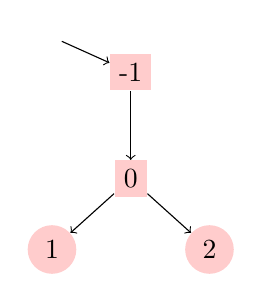
\begin{tikzpicture}[yscale=0.9]
\node (start) at (0,3) {};
\node[rectangle,fill=red!20] (-1) at (1,2.5) {-1};
\node[rectangle,fill=red!20] (0) at (1,1) {0};
\node[circle,fill=red!20] (1) at (0,0) {1};
\node[circle,fill=red!20] (2) at (2,0) {2};

\draw[->] (start)--(-1);
\draw[->] (-1)--(0);
\draw[->] (0)--(1);
\draw[->] (0)--(2);
\end{tikzpicture}
\end{center}
State~-1 is the initial state.  The states -1 and 0 are fully explored, and  states 1 and 2 are not fully explored.  The listener produces a file, the name of which is the name of the system under test with ``.tra'' as suffix (see \cite[Section 7.4]{B20}), with the following content.
\begin{verbatim}
-1 -> 0
0 -> 1
0 -> 2
1 2
\end{verbatim}
The first three lines describe the transitions.  Each line contains the source of the transition followed by the target of the transition.  The last line contains the states that are not fully explored yet.

\begin{franck}
\section{Counterexamples and Witnesses}


\end{franck}



\bibliographystyle{plain}
\bibliography{report}

\end{document}

%\section{Translation of CTL to normal forms}
%
%\description
%The objective of this project is to implement the translation of CTL to both normal forms developed in the "normal forms for CTL" project. 
%
%Implement a class named \lstinline{ExistentialNormalForm} that contains a static method named \lstinline{translate}.  This method takes as argument an object of type \lstinline{Formula}, which is part of the \lstinline{ctl} package.  The API of the \lstinline{ctl} package can be found \href{https://www.eecs.yorku.ca/course_archive/2020-21/W/4315/project/api/ast}{here} and has been implemented in the ``from parse tree to abstract syntax tree'' project.  Similarly, develop a class named \lstinline{PositiveNormalForm} that contains a static method named \lstinline{translate}.
%
%To represent a CTL formula in the normal forms, you may use classes of the \lstinline{ctl} package.  You may also add new classes to this package.  A CTL formula can be translated to its existential normal form as follows.
%\begin{lstlisting}
%Formula formula = ...
%Formula normalForm = ExistentialNormalForm.translate(formula);
%\end{lstlisting}
%
%\deliverables
%\begin{itemize}
%\item
%Properly documented Java code that implements both translations of CTL to the normal forms.
%\item
%A test suite, using JUnit, that rigorously tests the translations.
%\item
%A report describing the design, implementation, and testing of the translations.
%\end{itemize}
%
%
%\section{CTL model checking algorithm for partial transition systems}
%
%\description
%The objective of this project is to adjust the CTL model checking algorithm, as described in Section~6.4.1 of the textbook, to the setting of partial transition systems, as developed in the ``new semantics for CTL'' project.  Given a partial transition system and a CTL formula in existential normal form, as developed in the `` existential normal form for CTL'' project, the algorithm computes the corresponding satisfaction set.
%
%\resources
%\begin{itemize}
%\item 
%The textbook.
%\end{itemize}
%
%\deliverables
%\begin{itemize}
%\item 
%An algorithm, similar to Algorithm~14 of the textbook, for the computation of the satisfaction sets of CTL formulas in existential normal form for a partial transition system.
%\item
%A proof that proves the algorithm is correct, similar to Theorem~6.23 of the textbook.
%\item
%A report describing the algorithm and its correctness proof.
%\end{itemize}
%

%
%\section{Implementation of CTL model checking algorithm}
%
%\description
%The main objective of this project is to implement the algorithm developed in the ``CTL model checking algorithm for partial transition systems'' project.  As input, the algorithm takes a CTL formula in existential normal form, as implemented in the ``translation of CTL to existential normal form,'' and a partial transition system, provided by the `` JPF listener that writes a partial transition system to file.'' Another objective of this project is to design a simple GUI to import the file containing the partial transition system, to enter the CTL formula, and to run the implemented algorithm.
%
%\resources
%\begin{itemize}
%\item
%The textbook.
%\end{itemize}
%
%\deliverables
%\begin{itemize}
%\item 
%Properly documented Java code that implements the algorithm and the GUI.
%\item
%A test suite, using JUnit, that rigorously tests the implementation of the algorithm.
%\item
%A report describing the design, implementation, and testing of the algorithm.
%\end{itemize}


Bruns and Godefroid study partial Kripke structures in \cite{BG}.  These differ from ordinary transition system in their labelling function.  In our notation, $L : S \times \mathit{AP} \to \{ \top, \bottom, ? \}$.

According to Bruns and Godefroid, ``Obviously, any partial Kripke structure can be completed to obtain a traditional fully-defined Kripke structure, where $\varphi$ always evaluates to either true or false.  Some partial Kripke structures can only be completed to form Kripke structures that all satisfy the property $\varphi$, or to form Kripke structures that all violate $\varphi$ (this is the case, for instance but not exclusively, when $\varphi$ is a tautology or is unsatisfiable with a 2-valued interpretation).  Some other partial Kripke structures can be completed
to form Kripke structures that satisfy φ as well as Kripke structures that violate $\varphi$.''

Glenn Bruns and Patrice Godefroid
Model Checking Partial State Spaces with 3-Valued Temporal Logics

Glenn Bruns and Patrice Godefroid
Generalized Model Checking: Reasoning about Partial State Spaces


Kleene's strongest regular 3-valued propositional logic

Stephen Cole Kleene. Introduction to Metamathematics. North Holland,
1987.


One may be tempted to assume that these non-fully explored states \emph{have} unexplored transitions that are not part of the transition relation $\rightarrow$.  We will \emph{not} make the assumption that states which are not fully explored \emph{must have} outgoing transitions (they \emph{may have} them) because it complicates our algorithm as we will explain next.

Suppose that we were to assume that a non-fully explored state~$s$ must have at least one outgoing transition.  Assume we have not explored any of the outgoing transitions of state~$s$.  Then the formula $\exists \nxt \varphi$ holds in state~$s$ if and only if the CTL formula $\varphi$ is equivalent to $\TRUE$.  Deciding that $\varphi$ is equivalent to $\TRUE$ is the same as checking whether $\varphi$ is valid, which in turn is the same as checking that $\neg \varphi$ is not satisfiable.  However, the satisfiability problem for CTL is not easy to solve: it is EXPTIME-complete \cite{FL79}.



We first consider the formula $\forall \nxt \varphi$, where $\varphi$ is some arbitrary formula.  Assume that the state~$s$ is fully explored.  In that case,
\[
\satisfaction{\forall \nxt \varphi}(s) = \left \{
\begin{array}{ll}
\top & \mbox{if $\satisfaction{\varphi}(s') = \top$ for all $s \rightarrow s'$}\\
\bottom & \mbox{if $\satisfaction{\varphi}(s') = \bottom$ for some $s \rightarrow s'$}\\
? & \mbox{otherwise.}
\end{array}
\right .
\]
The above is equivalent to
\[
\satisfaction{\forall \nxt \varphi}(s) = \bigwedge \{\, \satisfaction{\varphi}(s') \mid s \rightarrow s' \,\}.
\]
Note that $\bigwedge \emptyset = \top$.

Next, assume that the state~$s$ is not fully explored.  Recall that state~$s$ has outgoing transitions, but those have not been explored yet.  We distinguish three cases.
\begin{itemize}
\item 
None of outgoing transitions of state~$s$ have been explored yet.  Let us first consider the case that $\varphi$ is $\TRUE$.  In that case, $\satisfaction{\forall \nxt \TRUE}(s) = \top$ because every state satisfies $\TRUE$.  Similarly, we have that $\satisfaction{\forall \nxt (\TRUE \vee \FALSE)}(s) = \top$.  To capture all these cases, we use the notion of equivalence of CTL formulas, denoted $\equiv$ (see \cite[Definition~6.12]{BK08}).  If $\varphi \equiv \TRUE$ then $\satisfaction{\forall \nxt \varphi}(s) = \top$.

Next, let us consider the case that $\varphi$ is $\FALSE$.  No state satisfies $\FALSE$.  Hence, $\satisfaction{\forall \nxt \FALSE}(s) = \bottom$.  More generally, $\varphi \equiv \FALSE$ then $\satisfaction{\forall \nxt \varphi}(s) = \bottom$.

Otherwise, $\varphi \not\equiv \TRUE$ and $\varphi \not\equiv \FALSE$.  The former implies that there exists a transition system with initial state $s_{\TRUE}$ such that $s_{\TRUE} \not\models \varphi$ and the latter implies that there exists a transition system with initial state $s_{\FALSE}$ such that $s_{\FALSE} \models \varphi$.  State~$s_0$ has at least one outgoing transition.  We do not know anything about the target state of that transition (it could be $s_{\TRUE}$ or $s_{\FALSE}$ or any other state), we do not know that value of $\satisfaction{\forall \nxt \varphi}(s)$.

Combining the above, we arrive at
\[
\satisfaction{\forall \nxt \varphi}(s) = \left \{
\begin{array}{ll}
\top & \mbox{if $\varphi \equiv \TRUE$}\\
\bottom & \mbox{if $\varphi \equiv \FALSE$}\\
? & \mbox{otherwise.}
\end{array}
\right .
\]
\item
State~$s$ has a single explored outgoing transition to state~$s_1$.  State~$s$ has more outgoing transitions, but those have not been explored yet.   As in the previous case, if  $\varphi \equiv \TRUE$ then $\satisfaction{\forall \nxt \varphi}(s) = \top$, and if $\varphi \equiv \FALSE$ then $\satisfaction{\forall \nxt \varphi}(s) = \bottom$.

Now let us consider state $s_1$ and formula $\varphi$.  If $\satisfaction{\varphi}(s_1) = \bottom$, we can conclude that $\satisfaction{\forall \nxt \varphi}(s) = \bottom$.  In case $\satisfaction{\varphi}(s) \not= \bottom$, we obtain no additional information about $\satisfaction{\forall \nxt \varphi}(s)$.

Combining the above, we arrive at
\[
\satisfaction{\forall \nxt \varphi}(s) = \left \{
\begin{array}{ll}
\top & \mbox{if $\varphi \equiv \TRUE$}\\
\bottom & \mbox{if $\varphi \equiv \FALSE$ or $\satisfaction{\varphi}(s_1) = \bottom$}\\
? & \mbox{otherwise.}
\end{array}
\right .
\]
Note that $\satisfaction{\varphi}(s_1) = \bottom$ if $\varphi \equiv \FALSE$.  Hence, we can simplify the above to
\[
\satisfaction{\forall \nxt \varphi}(s) = \left \{
\begin{array}{ll}
\top & \mbox{if $\varphi \equiv \TRUE$}\\
\bottom & \mbox{if $\satisfaction{\varphi}(s_1) = \bottom$}\\
? & \mbox{otherwise.}
\end{array}
\right .
\]
\item
State~$s$ has explored outgoing transitions to state~$s_1$ and $s_2$.  State~$s$ has more outgoing transitions, but those have not been explored yet.   As in the previous cases, if  $\varphi \equiv \TRUE$ then $\satisfaction{\forall \nxt \varphi}(s) = \top$, and if $\varphi \equiv \FALSE$ then $\satisfaction{\forall \nxt \varphi}(s) = \bottom$. 

Now let us consider state~$s_1$ and $s_2$.  If $\satisfaction{\varphi}(s_1) = \bottom$ or $\satisfaction{\varphi}(s_2) = \bottom$, we can conclude that $\satisfaction{\forall \nxt \varphi}(s) = \bottom$.  In case $\satisfaction{\varphi}(s_1)\not= \bottom$ and $\satisfaction{\varphi}(s_2)\not= \bottom$, we obtain no additional information about $\satisfaction{\forall \nxt \varphi}(s)$.  Therefore,
\[
\satisfaction{\forall \nxt \varphi}(s) = \left \{
\begin{array}{ll}
\top & \mbox{if $\varphi \equiv \TRUE$}\\
\bottom & \mbox{if $\varphi \equiv \FALSE$ or $\satisfaction{\varphi}(s_1) = \bottom$ or $\satisfaction{\varphi}(s_2) = \bottom$}\\
? & \mbox{otherwise.}
\end{array}
\right .
\]
This can be simplified to
\[
\satisfaction{\forall \nxt \varphi}(s) = \left \{
\begin{array}{ll}
\top & \mbox{if $\varphi \equiv \TRUE$}\\
\bottom & \mbox{if $\satisfaction{\varphi}(s_1) = \bottom$ or $\satisfaction{\varphi}(s_2) = \bottom$}\\
? & \mbox{otherwise.}
\end{array}
\right .
\]
\end{itemize}
The above three cases can be generalized as follows.
\[
\satisfaction{\forall \nxt \varphi}(s) = \left \{
\begin{array}{ll}
\top & \mbox{if $\varphi \equiv \TRUE$}\\
\bottom & \mbox{if $\varphi \equiv \FALSE$ or $\satisfaction{\varphi}(s') = \bottom$ for some $s \rightarrow s'$}\\
? & \mbox{otherwise.}
\end{array}
\right .
\]

This can be reformulated as follows.
\begin{align*}
\mathit{Sat}(\forall \nxt \varphi) & = 
\left \{
\begin{array}{ll}
S & \mbox{if $\varphi \equiv \TRUE$}\\
\{\, s \in F \mid \mathit{post}(s) \subseteq \mathit{Sat}(\varphi) \,\} & \mbox{otherwise}
\end{array}
\right .\\
\mathit{Unsat}(\forall \nxt \varphi) & = 
\left \{
\begin{array}{ll}
(S \setminus F) \cup \{\, s \in F \mid \mathit{post}(s) \not= \emptyset \,\}& \mbox{if $\varphi \equiv \FALSE$}\\
\{\, s \in S \mid \mathit{post}(s) \cap \mathit{Unsat}(\varphi) \not= \emptyset \,\} & \mbox{otherwise}
\end{array}
\right .\\
\mathit{Unknown}(\forall \nxt \varphi) & = S \setminus (\mathit{Sat}(\forall \nxt \varphi) \cup \mathit{Unsat}(\forall \nxt \varphi))
\end{align*}
In the above characterization we use
\[
\mathit{post}(s) = \{\, s' \in S \mid s \rightarrow s' \,\}.
\]

Next, let us consider the formula $\exists \nxt \varphi$, where $\varphi$ is some arbitary formula.  Assume that the state~$s$ is fully explored.  In that case,
\[
\satisfaction{\exists \nxt \varphi}(s) = \left \{
\begin{array}{ll}
\top & \mbox{if $\satisfaction{\varphi}(s') = \top$ for some $s \rightarrow s'$}\\
\bottom & \mbox{if $\satisfaction{\varphi}(s') = \bottom$ for all $s \rightarrow s'$}\\
? & \mbox{otherwise.}
\end{array}
\right .
\]
The above is equivalent to
\[
\satisfaction{\exists \nxt \varphi}(s) = \bigvee \{\, \satisfaction{\varphi}(s') \mid s \rightarrow s' \,\}.
\]
Note that $\bigvee \emptyset = \bottom$.

Next, assume that the state~$s$ is not fully explored.  Recall that state~$s$ has outgoing transitions, but those have not been explored yet.  We distinguish three cases.
\begin{itemize}
\item 
None of outgoing transitions of state~$s$ have been explored yet.  Let us first consider the case that $\varphi$ is $\TRUE$.  In that case, $\satisfaction{\exists \nxt \TRUE}(s) = \top$ because state~$s$ has outgoing transitions and every state satisfies $\TRUE$.  More generally, if $\varphi \equiv \TRUE$ then $\satisfaction{\exists \nxt \varphi}(s) = \top$.

Next, let us consider the case that $\varphi$ is $\FALSE$.  No state satisfies $\FALSE$.  Hence, $\satisfaction{\exists \nxt \FALSE}(s) = \bottom$.  More generally, $\varphi \equiv \FALSE$ then $\satisfaction{\exists \nxt \varphi}(s) = \bottom$.

Otherwise, $\varphi \not\equiv \TRUE$ and $\varphi \not\equiv \FALSE$.  The former implies that there exists a transition system with initial state $s_{\TRUE}$ such that $s_{\TRUE} \not\models \varphi$ and the latter implies that there exists a transition system with initial state $s_{\FALSE}$ such that $s_{\FALSE} \models \varphi$.  State~$s$ has at least one outgoing transition.  We do not know anything about the target state of that transition (it could be $s_{\TRUE}$ or $s_{\FALSE}$ or any other state), we do not know that value of $\satisfaction{\exists \nxt \varphi}(s)$.

Combining the above, we arrive at
\[
\satisfaction{\exists \nxt \varphi}(s) = \left \{
\begin{array}{ll}
\top & \mbox{if $\varphi \equiv \TRUE$}\\
\bottom & \mbox{if $\varphi \equiv \FALSE$}\\
? & \mbox{otherwise.}
\end{array}
\right .
\]
\item
State~$s$ has a single explored outgoing transition to state~$s_1$.  State~$s$ has more outgoing transitions, but those have not been explored yet.   As in the previous case, if  $\varphi \equiv \TRUE$ then $\satisfaction{\exists \nxt \varphi}(s) = \top$, and if $\varphi \equiv \FALSE$ then $\satisfaction{\exists \nxt \varphi}(s) = \bottom$.

Now let us consider state $s_1$ and formula $\varphi$.  If $\satisfaction{\varphi}(s_1) = \top$, we can conclude that $\satisfaction{\exists \nxt \varphi}(s) = \top$.  In case $\satisfaction{\varphi}(s_1)\not= \top$, we obtain no additional information about $\satisfaction{\exists \nxt \varphi}(s)$.

Combining the above, we arrive at
\[
\satisfaction{\exists \nxt \varphi}(s) = \left \{
\begin{array}{ll}
\top & \mbox{if $\varphi \equiv \TRUE$ or $\satisfaction{\varphi}(s_1) = \top$}\\
\bottom & \mbox{if $\varphi \equiv \FALSE$}\\
? & \mbox{otherwise.}
\end{array}
\right .
\]
Note that $\satisfaction{\varphi}(s_1) = \top$ if $\varphi \equiv \TRUE$.  Hence, we can simplify the above to
\[
\satisfaction{\exists \nxt \varphi}(s) = \left \{
\begin{array}{ll}
\top & \mbox{if $\satisfaction{\varphi}(s_1) = \top$}\\
\bottom & \mbox{if $\varphi \equiv \FALSE$}\\
? & \mbox{otherwise.}
\end{array}
\right .
\]
\item
State~$s$ has explored outgoing transitions to state~$s_1$ and $s_2$.  State~$s$ has more outgoing transitions, but those have not been explored yet.   As in the previous cases, if  $\varphi \equiv \TRUE$ then $\satisfaction{\exists \nxt \varphi}(s) = \top$, and if $\varphi \equiv \FALSE$ then $\satisfaction{\exists \nxt \varphi}(s) = \bottom$. 

Now let us consider state~$s_1$ and $s_2$.  If $\satisfaction{\varphi}(s_1) = \top$ or $\satisfaction{\varphi}(s_2) = \top$, we can conclude that $\satisfaction{\exists \nxt \varphi}(s) = \top$.  In case $\satisfaction{\varphi}(s_1)\not= \top$ and $\satisfaction{\varphi}(s_2)\not= \top$, we obtain no additional information about $\satisfaction{\exists \nxt \varphi}(s)$.  Therefore,
\[
\satisfaction{\exists \nxt \varphi}(s) = \left \{
\begin{array}{ll}
\top & \mbox{if $\varphi \equiv \TRUE$ or $\satisfaction{\varphi}(s_1) = \top$ or $\satisfaction{\varphi}(s_2) = \top$}\\
\bottom & \mbox{if $\varphi \equiv \FALSE$}\\
? & \mbox{otherwise.}
\end{array}
\right .
\]
This can be simplified to
\[
\satisfaction{\exists \nxt \varphi}(s) = \left \{
\begin{array}{ll}
\top & \mbox{if $\satisfaction{\varphi}(s_1) = \top$ or $\satisfaction{\varphi}(s_2) = \top$}\\
\bottom & \mbox{if $\varphi \equiv \FALSE$}\\
? & \mbox{otherwise.}
\end{array}
\right .
\]
\end{itemize}
The above three cases can be generalized as follows.
\[
\satisfaction{\exists \nxt \varphi}(s) = \left \{
\begin{array}{ll}
\top & \mbox{if $\varphi \equiv \TRUE$ or $\satisfaction{\varphi}(s') = \top$ for some $s \rightarrow s'$}\\
\bottom & \mbox{if $\varphi \equiv \FALSE$}\\
? & \mbox{otherwise.}
\end{array}
\right .
\]

This can be reformulated as follows.
\begin{align*}
\mathit{Sat}(\exists \nxt \varphi) & = 
\left \{
\begin{array}{ll}
S \setminus F \cup \{\, s \in F \mid \mathit{post}(s) \not= \emptyset \,\} & \mbox{if $\varphi \equiv \TRUE$}\\
\{\, s \in S \mid \mathit{post}(s) \cap \mathit{Sat}(\varphi) \not= \emptyset \,\} & \mbox{otherwise}
\end{array}
\right .\\
\mathit{Unsat}(\exists \nxt \varphi) & = 
\left \{
\begin{array}{ll}
S & \mbox{if $\varphi \equiv \FALSE$}\\
\{\, s \in F \mid \mathit{post}(s) \subseteq \mathit{Unsat}(\varphi) \,\} & \mbox{otherwise}
\end{array}
\right .\\
\mathit{Unknown}(\exists \nxt \varphi) & = S \setminus (\mathit{Sat}(\exists \nxt \varphi) \cup \mathit{Unsat}(\exists \nxt \varphi))
\end{align*}

Next, let us consider the formulas $\forall \always \varphi$.  Assume that the state $s$ is fully explored.  Then 
\[
\satisfaction{\forall \always \varphi}(s) = \left \{
\begin{array}{ll}
\top & \mbox{if $\satisfaction{\varphi}(s) = \top$ and $\satisfaction{\forall \always \varphi}(s') = \top$ for all $s \rightarrow s'$}\\
\bottom & \mbox{if $\satisfaction{\varphi}(s) = \bottom$ or $\satisfaction{\forall \always \varphi}(s') = \bottom$ for some $s \rightarrow s'$}\\
? & \mbox{otherwise.}
\end{array}
\right .
\]

Next, assume that the state $s$ is not fully explored.  Recall that state~$s$ has outgoing transitions, but those have not been explored yet.  We distinguish three cases.
\begin{itemize}
\item 
None of outgoing transitions of state~$s$ have been explored yet.  Let us first consider the case that $\varphi$ is $\TRUE$.  In that case, $\satisfaction{\forall \always \TRUE}(s) = \top$ because each (reachable) state satisfies $\TRUE$.

Next, let us consider the case that $\varphi$ is $\FALSE$.  No state satisfies $\FALSE$.  Hence, $\satisfaction{\forall \always \FALSE}(s) = \bottom$.  More generally, $\varphi \equiv \FALSE$ then $\satisfaction{\forall \always \varphi}(s) = \bottom$.

If $\satisfaction{\varphi}(s) = \bottom$, there exists a state reachable from state~$s$ that does not satisfy $\varphi$ and, hence, $\satisfaction{\forall \always \varphi}(s) = \bottom$.

Otherwise, $\varphi \not\equiv \TRUE$ and $\varphi \not\equiv \FALSE$.  The former implies that there exists a transition system with initial state $s_{\TRUE}$ such that $s_{\TRUE} \not\models \varphi$ and the latter implies that there exists a transition system with initial state $s_{\FALSE}$ such that $s_{\FALSE} \models \varphi$.  Hence, $\satisfaction{\forall \always \varphi}(s) = ?$.

Combining the above, we arrive at
\[
\satisfaction{\forall \always \varphi}(s) = \left \{
\begin{array}{ll}
\top & \mbox{if $\varphi \equiv \TRUE$}\\
\bottom & \mbox{if $\varphi \equiv \FALSE$ or $\satisfaction{\varphi}(s) = \bottom$}\\
? & \mbox{otherwise.}
\end{array}
\right .
\]
This can be further simplified to
\[
\satisfaction{\forall \always \varphi}(s) = \left \{
\begin{array}{ll}
\top & \mbox{if $\varphi \equiv \TRUE$}\\
\bottom & \mbox{if $\satisfaction{\varphi}(s) = \bottom$}\\
? & \mbox{otherwise.}
\end{array}
\right .
\]
\item
State~$s$ has a single explored outgoing transition to state~$s_1$.  State~$s$ has more outgoing transitions, but those have not been explored yet.   As in the previous case, if  $\varphi \equiv \TRUE$ then $\satisfaction{\forall \always \varphi}(s) = \top$, and if $\varphi \equiv \FALSE$ then $\satisfaction{\forall \always \varphi}(s) = \bottom$.

If $\satisfaction{\varphi}(s) = \bottom$, there exists a state reachable from state~$s$ that does not satisfy $\varphi$ and, hence, $\satisfaction{\forall \always \varphi}(s) = \bottom$.

Now let us consider state $s_1$.  If $\satisfaction{\forall \always \varphi}(s_1) = \bottom$, we can conclude that $\satisfaction{\forall \always \varphi}(s) = \bottom$.  In case $\satisfaction{\forall \always \varphi}(s_1)\not= \bottom$, we obtain no additional information about $\satisfaction{\forall \always \varphi}(s)$.

Combining the above, we arrive at
\[
\satisfaction{\forall \always \varphi}(s) = \left \{
\begin{array}{ll}
\top & \mbox{if $\varphi \equiv \TRUE$}\\
\bottom & \mbox{if $\varphi \equiv \FALSE$ or $\satisfaction{\varphi}(s) = \bottom$ or $\satisfaction{\forall \always \varphi}(s_1) = \bottom$}\\
? & \mbox{otherwise.}
\end{array}
\right .
\]
This can be further simplified to
\[
\satisfaction{\forall \always \varphi}(s) = \left \{
\begin{array}{ll}
\top & \mbox{if $\varphi \equiv \TRUE$}\\
\bottom & \mbox{if $\satisfaction{\varphi}(s) = \bottom$ or $\satisfaction{\forall \always \varphi}(s_1) = \bottom$}\\
? & \mbox{otherwise.}
\end{array}
\right .
\]
\item
State~$s$ has explored outgoing transitions to state~$s_1$ and $s_2$.  State~$s$ has more outgoing transitions, but those have not been explored yet.   As in the previous cases, if  $\varphi \equiv \TRUE$ then $\satisfaction{\forall \always \varphi}(s) = \top$, and if $\varphi \equiv \FALSE$ then $\satisfaction{\forall \always \varphi}(s) = \bottom$. 

If $\satisfaction{\varphi}(s) = \bottom$, there exists a state reachable from state~$s$ that does not satisfy $\varphi$ and, hence, $\satisfaction{\forall \always \varphi}(s) = \bottom$.

Now let us consider state~$s_1$ and $s_2$.  If $\satisfaction{\forall \always \varphi}(s_1) = \bottom$, we can conclude that $\satisfaction{\forall \always \varphi}(s) = \bottom$.  Similarly, if $\satisfaction{\forall \always \varphi}(s_2) = \bottom$, then $\satisfaction{\forall \always \varphi}(s) = \bottom$.  Otherwise, we obtain no additional information about $\satisfaction{\forall \always \varphi}(s)$.  Therefore,
\[
\satisfaction{\forall \always \varphi}(s) = \left \{
\begin{array}{ll}
\top & \mbox{if $\varphi \equiv \TRUE$}\\
\bottom & \mbox{if $\varphi \equiv \FALSE$ or $\satisfaction{\varphi}(s) = \bottom$ or $\satisfaction{\forall \always \varphi}(s_1) = \bottom$ or $\satisfaction{\forall \always \varphi}(s_2) = \bottom$}\\
? & \mbox{otherwise.}
\end{array}
\right .
\]
This can be further simplified to
\[
\satisfaction{\forall \always \varphi}(s) = \left \{
\begin{array}{ll}
\top & \mbox{if $\varphi \equiv \TRUE$}\\
\bottom & \mbox{if $\satisfaction{\varphi}(s) = \bottom$ or $\satisfaction{\forall \always \varphi}(s_1) = \bottom$ or $\satisfaction{\forall \always \varphi}(s_2) = \bottom$}\\
? & \mbox{otherwise.}
\end{array}
\right .
\]
\end{itemize}
The above three cases can be generalized as follows.
\[
\satisfaction{\forall \always \varphi}(s) = \left \{
\begin{array}{ll}
\top & \mbox{if $\varphi \equiv \TRUE$}\\
\bottom & \mbox{if $\satisfaction{\varphi}(s) = \bottom$ or $\satisfaction{\forall \always \varphi}(s') = \bottom$ for some $s \rightarrow s'$}\\
? & \mbox{otherwise.}
\end{array}
\right .
\]

Now consider that case that state~$s$ is not fully explored and transitions to itself and assume that $\varphi \not\equiv \FALSE$ and $\satisfaction{\varphi}(s) \not= \bottom$.  Then $\satisfaction{\forall \always \varphi}(s) = \bottom$ if $\satisfaction{\forall \always \varphi}(s) = \bottom$.  To demonstrate that $\satisfaction{\forall \always \varphi}$ can be defined so that it satisfies the above equation, we will rely on the Knaster-Tarski fixed-point theorem \cite{K28,T55}.

Let us first reformulate the above in terms of $\mathit{Sat}$, $\mathit{Unsat}$, and $\mathit{Unknown}$.  
\begin{align*}
\mathit{Sat}(\forall \always \varphi) & = 
\left \{
\begin{array}{ll}
S & \mbox{if $\varphi \equiv \TRUE$}\\
\{\, s \in F \mid s \in \mathit{Sat}(\varphi) \wedge \mathit{post}(s) \subseteq \mathit{Sat}(\forall \always \varphi) \,\} & \mbox{otherwise}
\end{array}
\right .\\
\mathit{Unsat}(\forall \always \varphi) & = 
\left \{
\begin{array}{ll}
(S \setminus F) \cup \{\, s \in F \mid \mathit{post}(s) \not= \emptyset \,\} & \mbox{if $\varphi \equiv \FALSE$}\\
\{\, s \in S \mid s \in \mathit{Unsat}(\varphi) \vee \mathit{post}(s) \cap \mathit{Unsat}(\forall \always \varphi) \not= \emptyset \,\} & \mbox{otherwise}
\end{array}
\right .\\
\mathit{Unknown}(\forall \always \varphi) & = S \setminus (\mathit{Sat}(\forall \always \varphi) \cup \mathit{Unsat}(\forall \always \varphi))
\end{align*}

To address the above observed circularity, we start with ordering sets of states, that is, the elements of $2^S$.  Clearly, we have that for all $U$, $V$, $W \in 2^S$,
\begin{itemize}
\item 
$U \subseteq U$,
\item
if $U \subseteq V$ and $V \subseteq U$ then $U = V$, and
\item
if $U \subseteq V$ and $V \subseteq W$ then $U \subseteq W$.
\end{itemize}

The set $2^S$ and the order $\subseteq$ form a complete lattice (see, for example, \cite[Section~6.1]{CGP99}).  Given a CTL formula~$\varphi$, with $\varphi \not\equiv \TRUE$, the function
\[
\mathcal{F}_{\varphi} : 2^S \to 2^S
\]
is defined by
\[
\mathcal{F}_{\varphi}(U) = \{\, s \in F \mid s \in \mathit{Sat}(\varphi) \wedge \mathit{post}(s) \subseteq U \,\}.
\]

Next, we show that the function $\mathcal{F}_{\varphi}$ is monotone, that is, for all $U$, $V \in 2^S$, if $U \subseteq V$ then $\mathcal{F}_{\varphi}(U) \subseteq \mathcal{F}_{\varphi}(V)$.  Let $U$, $V \in 2^S$ and assume that $U \subseteq V$.  Let $s \in \mathcal{F}_{\varphi}(U)$. To conclude that $\mathcal{F}_{\varphi}(U) \subseteq \mathcal{F}_{\varphi}(V)$, it remains to show that $s \in \mathcal{F}_{\varphi}(V)$.  Since $s \in \mathcal{F}_{\varphi}(U)$, we have that $s \in F$, $s \in \mathit{Sat}(\varphi)$, and $\mathit{post}(s) \subseteq U$.  Since $U \subseteq V$, we can conclude that $\mathit{post}(s) \subseteq V$.  Hence, $s \in \mathcal{F}_{\varphi}(V)$.

According to the Knaster-Tarski theorem, a monotone function on a complete lattice has a greatest fixed-point.  As we already observed above, the set $2^S $ with the order $\subseteq$ is a complete lattice.  Furthermore, we have shown that the function $\mathcal{F}_{\varphi}$ is monotone.  Hence, $\mathcal{F}_{\varphi}$ has a greatest fixed point.  A set $U \in 2^S$ is a fixed-point of $\mathcal{F}_{\varphi}$ if $\mathcal{F}_{\varphi}(U) = U$.  A set $U \in 2^S$ is a greatest fixed-point of $\mathcal{F}_{\varphi}$ if $U$ is a fixed-point of $\mathcal{F}_{\varphi}$ and for every fixed-point $V$ of $\mathcal{F}_{\varphi}$ we have that $V \subseteq U$.  We define $\mathit{Sat}(\forall \always \varphi)$ as the greatest fixed-point of $\mathcal{F}_{\varphi}$.

Since the set $2^S$ is finite, the Knaster-Tarski fixed point theorem also suggests an algorithm to compute the greatest fixed-point of $\mathcal{F}_{\varphi}$ since this greatest fixed point is equal to
\[
\bigcup \{\, U \in 2^S \mid U \subseteq \mathcal{F}_{\varphi}(U) \,\}.
\]
According to, for example, \cite[Section~6.2]{CGP99}, we can compute $\mathit{Sat}(\forall \always \varphi)$ as follows.
\begin{lstlisting}
$U = S$
repeat
  $U_{old} = U$
  $U = \{\, s \in F \mid s \in \mathit{Sat}(\varphi) \wedge \mathit{post}(s) \subseteq U \,\}$
until $U_{old} = U$
\end{lstlisting}

Given a CTL formula~$\varphi$, with $\varphi \not\equiv \FALSE$, the function
\[
\mathcal{G}_{\varphi} : 2^S \to 2^S
\]
is defined by
\[
\mathcal{G}_{\varphi}(U) = \{\, s \in S \mid s \in \mathit{Unsat}(\varphi) \wedge \mathit{post}(s) \cap U \not= \emptyset \,\}.
\]

Next, we show that the function $\mathcal{G}_{\varphi}$ is monotone, that is, for all $U$, $V \in 2^S$, if $U \subseteq V$ then $\mathcal{G}_{\varphi}(U) \subseteq \mathcal{G}_{\varphi}(V)$.  Let $U$, $V \in 2^S$ and assume that $U \subseteq V$.  Let $s \in \mathcal{G}_{\varphi}(U)$. To conclude that $\mathcal{G}_{\varphi}(U) \subseteq \mathcal{G}_{\varphi}(V)$, it remains to show that $s \in \mathcal{G}_{\varphi}(V)$.  Since $s \in \mathcal{G}_{\varphi}(U)$, we have that $s \in S$, $s \in \mathit{Unsat}(\varphi)$ and $\mathit{post}(s) \cap U \not= \emptyset$.  Since $U \subseteq V$, we can conclude that $\mathit{post}(s) \cap V \not= \emptyset$.  Hence, $s \in \mathcal{G}_{\varphi}(V)$.

According to the Knaster-Tarski theorem, a monotone function on a complete lattice has a least fixed-point.  Since the set $2^S$ is finite, the Knaster-Tarski fixed point theorem also suggests an algorithm to compute the least fixed-point of $\mathcal{G}_{\varphi}$ since this least fixed point is equal to
\[
\bigcap \{\, U \in 2^S \mid \mathcal{G}_{\varphi}(U) \subseteq U \,\}.
\]
According to, for example, \cite[Section~6.2]{CGP99}, we can compute $\mathit{Unsat}(\forall \always \varphi)$ as follows.
\begin{lstlisting}
$U = \emptyset$
repeat
  $U_{old} = U$
  $U = \{\, s \in S \mid s \in \mathit{Unsat}(\varphi) \wedge \mathit{post}(s) \cap U \not= \emptyset \,\}$
until $U_{old} = U$
\end{lstlisting}

Next, let us consider the formulas $\exists \always \varphi$.  Assume that the state $s$ is fully explored.  Then 
\[
\satisfaction{\exists \always \varphi}(s) = \left \{
\begin{array}{ll}
\top & \mbox{if $\satisfaction{\varphi}(s) = \top$ and ($s \not\rightarrow$ or $\satisfaction{\exists \always \varphi}(s') = \top$ for some $s \rightarrow s'$)}\\
\bottom & \mbox{if $\satisfaction{\varphi}(s) = \bottom$ or ($s \rightarrow$ and $\satisfaction{\exists \always \varphi}(s') = \bottom$ for all $s \rightarrow s'$)}\\
? & \mbox{otherwise.}
\end{array}
\right .
\]

Next, assume that the state $s$ is not fully explored.  Then
\[
\satisfaction{\exists \always \varphi}(s) = \left \{
\begin{array}{ll}
\top & \mbox{if $\varphi \equiv \TRUE$ or ($\satisfaction{\varphi}(s) = \top$ and $\satisfaction{\exists \always \varphi}(s') = \top$ for some $s \rightarrow s'$)}\\
\bottom & \mbox{if $\satisfaction{\varphi}(s) = \bottom$}\\
? & \mbox{otherwise.}
\end{array}
\right .
\]

Let us first reformulate the above in terms of $\mathit{Sat}$, $\mathit{Unsat}$, and $\mathit{Unknown}$.  
\begin{align*}
\mathit{Sat}(\exists \always \varphi) = & 
\{\, s \in S \mid s \in \mathit{Sat}(\varphi) \wedge \mathit{post}(s) \cap \mathit{Sat}(\exists \always \varphi) \not= \emptyset \,\} \cup\\
& \{\, s \in F \mid s \in \mathit{Sat}(\varphi) \wedge \mathit{post}(s) = \emptyset \,\}\\
\mathit{Unsat}(\exists \always \varphi) = & 
\mathit{Unsat}(\varphi) \cup \{\, s \in F \mid \emptyset \not= \mathit{post}(s) \subseteq \mathit{Unsat}(\varphi) \,\}\\
\mathit{Unknown}(\exists \always \varphi) = & S \setminus (\mathit{Sat}(\exists \always \varphi) \cup \mathit{Unsat}(\exists \always \varphi))
\end{align*}

The set $\mathit{Sat}(\exists \always \varphi)$ can be defined as a greatest fixed-point.  
%The set $\mathit{Unsat}(\exists \always \varphi)$ can be defined as a ??? fixed-point.

\color{black}

\textcolor{blue}{Similarly, we might be able to characterize $\mathit{Unsat}(\forall \always \varphi)$ as a least fixed-point.}
